\documentclass{article}
\usepackage{iclr2027_conference,times}
\usepackage[utf8]{inputenc}
\usepackage[T1]{fontenc}
\usepackage[english]{babel}
\usepackage{amsmath,amssymb,mathrsfs}
\usepackage{enumitem}
\usepackage{booktabs}
\usepackage{longtable}
\usepackage{array}
\usepackage{graphicx}
\usepackage{tikz}
\usepackage{xcolor}
\usepackage{placeins}
\usepackage{float}
\usepackage[hidelinks]{hyperref}
\usepackage{url}
\usepackage{comment}


\title{PRESTO: Perspective-Based Entropy--Sparsity Training Optimization}
% The ICLR submission style hides this field during double-blind review.
\author{Anonymous authors}

\usepackage{multirow}
\usepackage{amsthm}
\newtheorem{proposition}{Proposition}
\usepackage{algorithm}
\usepackage{algpseudocode}
\setlength{\textfloatsep}{5pt plus 1pt minus 1pt}
\setlength{\intextsep}{5pt plus 1pt minus 1pt}
\setlength{\abovecaptionskip}{4pt}
\setlength{\belowcaptionskip}{2pt}
\usepackage{pgfplots}
\pgfplotsset{compat=1.17}
\begin{document}
\raggedbottom
\maketitle

\begin{abstract}
Pruning and quantization are the two standard ways of making a neural network
smaller, but the entropy of the representation that they produce is rarely part
of what training optimizes. We introduce PRESTO, a quantization-aware training
method that trains against a surrogate, defined through a convex inner problem, of
the size the weights will occupy after lossless coding. Uniform quantization with learned step sizes is combined
with an inner problem, in perspective form, that trades the mass each weight
places on the non-zero symbols against a convex penalty on their relaxed counts,
the two channels into which that coded size decomposes. Because those counts couple every weight of a
tensor, we relax the count constraints in a Lagrangian way, which separates the
inner problem into one subproblem per symbol and one per weight, both solved
exactly at a fixed multiplier at a cost linear in the number of symbols. The
envelope derivatives of the relaxed value function then give gradients for the
latent weights and for the step sizes, so that the network, the grid and the
symbol distribution move together, and since the dual is advanced by a few
warm-started steps rather than solved, that direction is an exact subgradient of a
Lagrangian lower bound of the regularizer as the solver poses it. Measured against matched controls,
PRESTO reduces the size of a quantized network while its accuracy stays above the
full-precision checkpoint, reaching $4.89\%$ of the checkpoint on ResNet-18 and
$5.12\%$ on ResNet-50 against controls at $9.84\%$ and $9.97\%$ trained on the same
budget, which the recipe without the regularizer instead makes larger, and
$4.24\%$ on ResNet-18 once the schedule is extended to a hundred epochs. On the
architectures whose control already falls below full precision we report
the frontier against that control: DeiT-Small reaches $9.06\%$ from a control at
$11.99\%$, EfficientNet-B0 reaches $10.15\%$ at $76.820$ top-1 where the
reference implementation of ISO/IEC 15938-17 reports $76.780$ at $11.25\%$, and
ViT-B/16 delivers $80.372\%$ top-1 at $4.41\%$ of the checkpoint where the same
codec reports $75.22\%$ at $4.85\%$.
\end{abstract}

\section{Introduction}
\label{sec:introduction}

Model compression works through three complementary mechanisms, since pruning
removes parameters, quantization represents the surviving values with a finite
codebook, and lossless coding removes the statistical redundancy that is left in
the resulting stream of symbols. The classical Deep Compression pipeline applies
the three in sequence \citep{han2016deep}, and its success raises the design
question that we take up here: should a network be compressed after it has been
trained, or should its compressibility shape the training objective itself?

Quantization-aware training follows the second principle by simulating
low-precision arithmetic while the network is being optimized, so that PACT
learns the clipping range of the activations \citep{choi2018pact} and LSQ
optimizes the quantization scales directly \citep{esser2020lsq}, while
post-training methods such as HAWQ \citep{dong2019hawq}, BRECQ
\citep{li2021brecq} and L$^2$ \citep{shi2023l2} avoid retraining altogether by
reconstructing each layer locally. All of these methods control distortion or hardware precision, and none
of them controls entropy, although a representation with few bits per weight
need not have low entropy: two models that use the same codebook can produce
symbol streams whose compressed sizes are very different. Entropy-aware
compression addresses that difference explicitly. Entropy-constrained training
writes the size of the model into the objective \citep{wiedemann2018entropy},
DeepCABAC combines rate-distortion quantization with context-adaptive coding
\citep{wiedemann2019deepcabac}, and the same coding engine has since become
ISO/IEC 15938-17 and the open-source NNCodec \citep{becking2023nncodec}, which is
the natural reference for any claim about size after lossless coding, while CERWU
\citep{conzelmann2025rate} improves on that standard by $20$ to $40\%$ in bit rate
on convolutional networks. Code length is therefore an established target rather
than a by-product of the nominal bit width, but all of these methods act after
training has finished, on a checkpoint that they did not shape.

A second family of methods shapes the representation while the network is being
trained. Entropy penalized reparameterization \citep{oktay2020epr} learns the
weights in a latent space that has its own probability model and entropy penalty,
and on ResNet-18 it is, as far as we know, the smallest lossless entropy-coded
model that has been published, at $4.22\%$ of the checkpoint, while LilNetX
\citep{girish2023lilnetx} adds structured sparsity to the same formulation and
reaches $2.16\%$ at $1.2$ points below its own baseline. Both of them rebuild a
dense full-precision network at deployment time, so they save storage without
producing a low-precision model, whereas PRESTO returns a genuine four-bit
codebook, eight bits on the few tensors listed in Section~\ref{sec:experiments},
whose symbol stream is what the encoder actually sees. The closest
method to our objective is HEMP \citep{tartaglione2021hemp}, which adds a
differentiable entropy term to the loss. PRESTO differs from it in three ways: the
inner problem is solved exactly at a fixed multiplier instead of being smoothed,
so the gradient is an envelope derivative of the relaxed value function rather
than of a surrogate; sparsity and the symbol
distribution are controlled by a single relaxation instead of an entropy term
paired with a separate pruning stage; and the same derivatives are applied to the
learned step sizes, so the grid moves along with the weights. In concurrent work,
CoDeQ \citep{wenshoj2025codeq} observes that the dead zone of a scalar quantizer
is exactly magnitude pruning and learns its width by backpropagation, which is
the mechanism that our sparsity term also uses, although it reports bit
operations rather than coded size. Learning the accuracy, the sparsity, the
quantization levels and the symbol distribution at the same time remains
difficult, because the symbol counts couple every weight that shares a codebook.

PRESTO handles that coupling with perspective optimization. Perspective
reformulations have already produced effective regularizers for structured
pruning \citep{cacciola2023deep}, and we extend the idea from a binary
keep-or-remove decision to a relaxed assignment over the quantization symbols, so
that the inner problem represents each latent weight, controls the mass that the
weight places on non-zero symbols and aggregates the global symbol counts. A
Lagrangian relaxation of the count constraints then splits the tensor-level
problem into per-symbol and per-weight subproblems that can be solved in
parallel, while the envelope derivatives make the resulting value function usable
inside ordinary gradient-based training once the dual has been advanced.

Our contributions are the following. We formulate a perspective, entropy-aware
regularizer that couples sparsity and the symbol distribution inside learned-step
quantization, and we derive a Lagrangian decomposition whose inner problem is
solved exactly in closed form at $O(C)$ per weight, with envelope derivatives for
the latent weights and for the learned step sizes and an explicit account of what
those derivatives are exact for when the dual is truncated. Measuring against matched
controls on the five architectures of Table~\ref{tab:main}, we show that the
regularizer halves the
serialized size of a quantized network while its accuracy stays above the
full-precision checkpoint, although the same training without the regularizer
makes the model larger. A term ablation on two architectures then shows that
which of the two coefficients is sufficient on its own is a property of the
architecture and not of the method, since the sparsity term alone recovers
$97.5\%$ of the compression on AlexNet but only $58.1\%$ on ResNet-18, where the
entropy term instead recovers $97.2\%$. We also report what the method does not
do, including the one architecture on which published work is still ahead of us
and our diagnosis of the reason.

\paragraph{Outline.} Sections~\ref{sec:method} and~\ref{sec:optimization} state
the method and its optimization, and Section~\ref{sec:experiments} reports the
experiments. Appendix~\ref{app:experimental-details} documents the training
implementation and every run: its configuration,
the quantized fraction of each checkpoint, the two term-ablation tables, the cost
of the support mask, notes on the transfer architectures, the wall-clock cost and
the learning curves. Appendix~\ref{app:more-experiments} reports the remaining
experiments in full, from the measurement that quantization-aware training on its
own makes models larger to the comparison between the joint objective and the same
objective split into two stages, the transformer frontiers, the two mechanisms,
the cost of per-channel grids and the negative results.
Appendix~\ref{app:derivations} gives every derivation,
Appendix~\ref{app:hyper} the procedure by which the coefficients are calibrated,
Appendix~\ref{app:consistency} what is held identical across architectures and
what is not, and Appendix~\ref{app:notation} the glossary of notation.

\section{PRESTO Method}
\label{sec:method}

\subsection{Setting, Notation and the Quantizer}
\label{sec:setting}
\label{sec:lsq}

Let $f(\cdot;\theta)$ be a network whose parameters divide into the weight
tensors that we quantize, indexed by $\Lambda$, and the remaining
floating-point parameters $\theta_{\mathrm{fp}}$, which are the biases and the
normalization parameters. Tensor $\ell\in\Lambda$ has $n_\ell$ entries indexed by
$i\in\mathcal I_\ell$ and latent weights $w^{(\ell)}$, and tensor $\ell$ uses a codebook of cardinality
$C_\ell$, of which $\mathcal B$ denotes the $B_\ell:=C_\ell-1$ non-zero symbols;
we drop the subscript wherever one tensor is under discussion, which is everywhere
below.
We keep the zero symbol separate from that set, because the relaxation of
Section~\ref{sec:metaq-value} represents it by a mass $z_i^{(\ell)}$ instead of by
an element of $\mathcal B$. The task loss $\mathcal L_{\mathrm{task}}$ is the
usual cross-entropy risk, and Appendix~\ref{app:notation} lists every symbol that
we use.

We build on LSQ \citep{esser2020lsq}, in which each tensor carries a single
positive step size $a_\ell$ that is learned together with the weights. A latent
weight is mapped onto the integer grid by $r_i^{(\ell)}:=w_i^{(\ell)}/a_\ell$,
then clipped to $[Q_n,Q_p]$, rounded and scaled back, so that the value that is
deployed is
$\widehat w_i^{(\ell)}=a_\ell\,\mathrm{clip}(\lfloor r_i^{(\ell)}\rceil,Q_n,Q_p)$
and the clipped latent weight is
$\bar w_i^{(\ell)}:=a_\ell\,\mathrm{clip}(r_i^{(\ell)},Q_n,Q_p)$. A per-channel
variant, in which $a_\ell$ becomes one step size per output channel, is used only
by the superseded controls of Table~\ref{tab:cross-architecture} and is priced in
Appendix~\ref{sec:per-channel-twice}; every run of Tables~\ref{tab:main} to
\ref{tab:extra} is per-tensor. The
rounding is to nearest with ties to even and is handled in the backward pass by a
straight-through estimator. With that convention the deployed value is the zero
symbol exactly when
\begin{equation}
  \left|w_i^{(\ell)}\right|\leq\tfrac{1}{2}a_\ell,
  \label{eq:lsq-zero-symbol}
\end{equation}
so that every zero reported in this paper is produced by that rule and by no
external pruning step. Appendix~\ref{app:lsq-details} gives the grid, the codebook
values $v_b^{(\ell)}=a_\ell q_b$ and the initialization of $a_\ell$ in full.

\subsection{Perspective and Entropy-Based Regularizer}
\label{sec:metaq-value}

Define the set of nonzero symbols as
\[
  \mathcal B:=\mathcal Q\setminus\{0\},
  \qquad B:=|\mathcal B|=C-1.
\]
The letter $b$ indexes an element of $\mathcal B$, and $q_b$ is the
corresponding integer code. In tensor $\ell$, the real-valued level associated
with symbol $b$ is
\begin{equation}
  v_b^{(\ell)}(a_\ell):=a_\ell q_b.
  \label{eq:real-level}
\end{equation}

For every pair $(i,b)\in\mathcal I_\ell\times\mathcal B$ we introduce a
non-negative assignment mass $x_{i,b}^{(\ell)}$, and write
$y_i^{(\ell)}\in[0,1]$ for the total mass with which weight $i$ is represented by
non-zero symbols, $z_i^{(\ell)}:=1-y_i^{(\ell)}$ for the mass on the zero symbol,
and $c_b^{(\ell)}\geq0$ for the relaxed count of symbol $b$. Below, $a_\ell$ and
$\bar w^{(\ell)}(a_\ell)$ are arguments while $x^{(\ell)},y^{(\ell)},c^{(\ell)}$
are the variables of the inner minimization, and $T_1,T_2,T_3\geq0$ are the three
coefficients. We define\footnote{With the continuous extension
$0\log_2 0:=0$.}
\begin{align}
 \Phi_\ell(\bar w^{(\ell)},a_\ell)
 :=\min_{x^{(\ell)},y^{(\ell)},c^{(\ell)}}\quad&
 T_1\sum_{i\in\mathcal I_\ell}
      \frac{(\bar w_i^{(\ell)})^2}{y_i^{(\ell)}}
 +T_2\sum_{i\in\mathcal I_\ell}y_i^{(\ell)}
 +T_3\sum_{b\in\mathcal B}
      c_b^{(\ell)}\log_2 c_b^{(\ell)}
 \label{eq:metaq-value}\\
 \text{s.t.}\quad&
 \sum_{b\in\mathcal B}
 v_b^{(\ell)}(a_\ell)x_{i,b}^{(\ell)}
 =\bar w_i^{(\ell)},
 &&\hspace{-3em} i\in\mathcal I_\ell,
 \label{eq:representation}\\
 &
 \sum_{b\in\mathcal B}x_{i,b}^{(\ell)}
 =y_i^{(\ell)},
 &&\hspace{-3em} i\in\mathcal I_\ell,
 \label{eq:mass}\\
 &
 c_b^{(\ell)}
 =\sum_{i\in\mathcal I_\ell}x_{i,b}^{(\ell)},
 &&\hspace{-3em} b\in\mathcal B,
 \label{eq:counts}\\
 &
 x_{i,b}^{(\ell)}\geq0,
 \quad 0\leq y_i^{(\ell)}\leq1,
 &&\hspace{-3em} i\in\mathcal I_\ell,\; b\in\mathcal B.
 \label{eq:domain}
\end{align}
The $T_1$ term uses the closed extension of $u^2/y$: it equals $u^2/y$ for
$y>0$, is $0$ at $(u,y)=(0,0)$ and $+\infty$ when $y=0$ with $u\neq0$, which
makes explicit that a weight can carry zero mass only when the weight itself is
zero.

The three coefficients play different roles. $T_1$ weights the perspective ridge,
$T_2$ penalizes the mass assigned to non-zero symbols, and $T_3$ weights the term
we call the entropy term, by which we mean the convex penalty
$\sum_b c_b^{(\ell)}\log_2 c_b^{(\ell)}$ on the relaxed counts and nothing more.
It deserves a precise statement, because that sum is not the entropy of the
non-zero symbols and minimizing it does not minimize that entropy. Writing
$m=\sum_b c_b^{(\ell)}$, the ideal zero-order code length of a tensor is
$n_\ell H(m/n_\ell)+mH(c^{(\ell)}/m)$, the mask plus the value stream, which is
$n_\ell$ times the entropy of the distribution over all $C_\ell$ symbols with the
zero symbol included, and it is a proxy for what the coder produces rather than
that size itself (Appendix~\ref{app:mask-cost}). Since $c\mapsto c\log_2c$ is minimized at $c=1/e$,
our term prices every non-zero symbol and pushes mass into the excluded zero
symbol, which is the channel through which it lowers that entropy, while at a
fixed $m$ it acts weakly the other way because the same sum is minimized at
uniform counts. Appendix~\ref{app:count-penalty} gives the arithmetic.
The values of the coefficients are not part of the definition of
the method and are given only in the experimental protocol. The zero symbol is excluded from $\mathcal B$ and is
represented only by $z_i^{(\ell)}$, which prevents the same zero value from
having two different representations.

Inside the training procedure $z_i^{(\ell)*}$ is a relaxed variable of the inner
problem rather than a hard pruning decision, so it contributes to the PRESTO
subgradient but never overwrites a latent weight with zero: PRESTO reshapes the
latent distribution towards the region that the quantizer maps to zero, and LSQ
is what produces the zeros seen in the forward pass and in the deployed model.

The outer PRESTO objective is
$\min_{w,a,\theta_{\mathrm{fp}}}\mathcal J$ with
\begin{equation}
  \mathcal J(w,a,\theta_{\mathrm{fp}})
  :=
  \mathcal L_{\mathrm{task}}\!\left(\widehat w(a),\theta_{\mathrm{fp}}\right)
  +\underbrace{\sum_{\ell\in\Lambda}
   \Phi_\ell\!\left(\bar w^{(\ell)}(a_\ell),a_\ell\right)}
   _{\textstyle \mathcal R_{\mathrm{PRESTO}}(w,a)}.
  \label{eq:outer-objective}
\end{equation}
The task loss contributes its ordinary gradient, and the regularizer contributes a
subgradient
$\nabla_{\mathrm{PRESTO}}\in\partial_{(w,a)}\mathcal R_{\mathrm{PRESTO}}\times\{0\}$
in which the zero appears because $\mathcal R_{\mathrm{PRESTO}}$ does not depend
on the floating-point parameters, and the sum of the two lies in
$\partial\mathcal J$. That is the direction we would follow if the inner problem
were solved to optimality; Section~\ref{sec:optimization} derives its components
and states what a truncated dual delivers instead.

\section{Optimization}
\label{sec:optimization}

\subsection{Lagrangian Relaxation and Decomposition}
\label{sec:lagrangian-decomposition}

The inner problem of Eq.~\eqref{eq:metaq-value} contains one set of variables for
every weight and a second set that is shared across the tensor. The
representation and mass constraints of Eqs.~\eqref{eq:representation} and
\eqref{eq:mass} involve a single weight index $i$, whereas each count constraint
of Eq.~\eqref{eq:counts} couples all the weights through the sum
$c_b^{(\ell)}=\sum_{i\in\mathcal I_\ell}x_{i,b}^{(\ell)}$, so that solving the
inner problem directly would mean handling every assignment mass of a tensor at
once. Lagrangian relaxation removes exactly that global coupling.

Fix a tensor $\ell\in\Lambda$, a clipped latent-weight vector
$\bar w^{(\ell)}$ and a step size $a_\ell$. Attaching an unrestricted multiplier
$\xi_b^{(\ell)}\in\mathbb R$ to each count constraint and dualizing only those
constraints gives a partial Lagrangian whose minimum over the remaining feasible
variables is the dual function
$\varphi^{(\ell)}_{\bar w^{(\ell)},a_\ell}(\xi^{(\ell)})$, concave as a pointwise
infimum of affine functions of the multipliers. Appendix~\ref{app:decomposition}
carries the algebra; the result is that it splits:
\begin{align}
 \varphi_{\bar w^{(\ell)},a_\ell}^{(\ell)}(\xi^{(\ell)})
 ={}&
 \sum_{b\in\mathcal B}
 \min_{c_b^{(\ell)}\geq0}
 \left\{
   T_3c_b^{(\ell)}\log_2c_b^{(\ell)}
   -\xi_b^{(\ell)}c_b^{(\ell)}
 \right\}
 \notag\\
 &+\sum_{i\in\mathcal I_\ell}
 \min_{(x_i^{(\ell)},y_i^{(\ell)})\in
       \mathcal F_i^{(\ell)}}
 \left\{
   T_1\frac{(\bar w_i^{(\ell)})^2}{y_i^{(\ell)}}
   +T_2y_i^{(\ell)}
   +\sum_{b\in\mathcal B}
      \xi_b^{(\ell)}x_{i,b}^{(\ell)}
 \right\},
 \label{eq:dual-decomposition}
\end{align}
where $x_i^{(\ell)}=(x_{i,b}^{(\ell)})_{b\in\mathcal B}$, and
$\mathcal F_i^{(\ell)}$ is the local feasible set
\begin{equation}
 \mathcal F_i^{(\ell)}
 :=
 \left\{
 (x_i^{(\ell)},y_i^{(\ell)}):
 \begin{array}{l}
 x_{i,b}^{(\ell)}\geq0\quad \text{for every }b\in\mathcal B,\\
 0\leq y_i^{(\ell)}\leq1,\\
 \sum_{b\in\mathcal B}v_b^{(\ell)}(a_\ell)x_{i,b}^{(\ell)}
     =\bar w_i^{(\ell)},\\
 \sum_{b\in\mathcal B}x_{i,b}^{(\ell)}=y_i^{(\ell)}
 \end{array}
 \right\}.
 \label{eq:local-feasible-set}
\end{equation}
The first line consists of $B$ independent one-dimensional count subproblems, one
for each non-zero symbol, and the second consists of $n_\ell$ independent
per-weight subproblems that share the multiplier but no optimization variables,
so that once $\xi^{(\ell)}$ is fixed the tensor-level problem can be solved in
parallel across symbols and across weights, which is the reason for relaxing it
in the first place. The dual problem is
\begin{equation}
  \max_{\xi^{(\ell)}\in\mathbb R^B}
  \varphi_{\bar w^{(\ell)},a_\ell}^{(\ell)}(\xi^{(\ell)}),
  \label{eq:lagrangian-dual}
\end{equation}
and it is exact: the objective is convex and closed, the constraints are affine
and the feasible set is compact, so the value of the perturbed problem is lower
semicontinuous at the origin and no duality gap remains.
Proposition~\ref{prop:strong-duality}, in Appendix~\ref{app:strong-duality},
proves this and separates the two roles the hypotheses play, since clipping the latent weights is what makes the problem
feasible with finite value while a single weight strictly inside the representable
interval is what makes the dual optimum attained. The relaxation therefore changes
the way the inner problem is solved without changing its value. Finally,
for a fixed $\xi^{(\ell)}$ the difference between the counts that the per-weight
solutions reconstruct and the counts that the count subproblems return is a
supergradient of $\varphi_{\bar w^{(\ell)},a_\ell}^{(\ell)}$, and that difference
drives the dual iteration described below.

\subsection{Per-Weight Solution, Gradients and Dual Update}
\label{sec:per-weight-subproblem}
\label{sec:joint-gradients}
\label{sec:optimization-order}

For a fixed multiplier the per-weight subproblem is a linear knapsack over the
$B$ non-zero symbols together with the zero symbol, and it is solved exactly in
closed form. Every candidate symbol contributes a pair $(v_b,\xi_b)$, the optimum
is reached at a vertex of the lower convex hull of those pairs, so the assignment
mass concentrates on at most two adjacent symbols, and the optimal non-zero mass
$y_i^\star$ then follows from a one-dimensional minimization of a perspective
term against a linear one, at a cost of $O(C)$ per weight and with no iteration
at all. Appendix~\ref{app:subproblem} states the breakpoints, proves that the
vertices of the hull are the only candidates and gives the closed form of
$y_i^\star$, and Algorithm~\ref{alg:hull}, in Appendix~\ref{app:algorithms}, is
the solver that follows from it.

At a fixed multiplier the two families of subproblems are solved exactly, so
Danskin's theorem applies to the inner minimization and the derivative that
enters training is an \emph{envelope} derivative evaluated at the inner optimum
rather than the derivative of a smoothed surrogate. For the latent weights it is
\begin{equation}
  \beta^\star_i \;=\; \mu_i \;+\; \frac{2T_1\,\bar w_i}{y_i^\star},
  \label{eq:beta-star}
\end{equation}
where $\mu_i$ collects the multiplier of the symbols to which the weight is
assigned, and the step sizes receive the matching derivative through the
dependence of $v_b$ on $a_\ell$, so that the network, the quantization grid and
the symbol distribution all move within one backward pass
(Appendices~\ref{app:weight-grad}--\ref{app:total-grad}).

Two qualifications belong with that statement. Because we advance the dual by
$N_{\mathrm{dual}}$ warm-started steps per call rather than solving it, the
expression is an exact subgradient of the \emph{relaxed} value function at the
multiplier we hold and an inexact proxy for $\Phi_\ell$, the count residual being
our diagnostic for the gap rather than a bound on it; and the solver boxes the
relaxed counts and projects the multiplier onto the matching interval, so the
problem it poses is not literally Eq.~\eqref{eq:metaq-value} and the ascent runs
on the projected dual of that boxed problem. Appendix~\ref{app:boxed} states both
differences precisely.

The multiplier itself is updated by normalized supergradient ascent with warm
starts, for $N_{\mathrm{dual}}$ iterations every \texttt{entropy\_every}
optimizer steps, using the count residual divided by $n_\ell$ as the
supergradient. One property of that update deserves attention, because the
interval the multiplier has to cross is proportional to $T_3$ while a step of
fixed absolute size is not, so raising the entropy coefficient moves the target
away just as fast as it raises it and the term becomes weaker rather than
stronger. Measuring the step as a fraction of the dual range removes that
dependence and every run in this paper uses the relative step;
Appendix~\ref{app:dual-rate} derives the rate and
Appendix~\ref{sec:negative} reports the runs on which we found the
problem.

\section{Experiments}
\label{sec:experiments}

\subsection{Evaluation Protocol}

The question we ask throughout is whether PRESTO makes quantized weights smaller
after lossless coding at the same accuracy and the same training budget. Every
run starts from a public full-precision checkpoint, quantizes all the
convolutional and linear weight tensors and keeps the activations in FP32, and we
never apply a pruning rule, so every zero is produced by
Eq.~\eqref{eq:lsq-zero-symbol} and the sparsity is emergent. The training
machinery around that objective, the optimizers and schedules, the distillation
and the batch-norm recalibration, is implementation rather than method and is
stated in Appendix~\ref{sec:training-implementation}. The codebook has $C_\ell=16$
symbols everywhere except on the two input convolutions of AlexNet and the input
and depthwise convolutions of EfficientNet-B0, $0.07\%$ and $3.7\%$ of their
weights, which use eight bits and are counted at their true cost in every ratio. Each number is the final
epoch of a single run unless we say otherwise.

\paragraph{Size is measured rather than nominal, and over the whole checkpoint.}
The \emph{packet} is the complete serialized artifact, containing the support
mask, the stream of non-zero symbols and the metadata, the learned step sizes
included; a nominal bit width would hide both the gain from entropy coding and the
cost of the metadata. Published methods report megabytes for the whole checkpoint,
so we do the same: if $f$ is the fraction of parameters we quantize, a packet of
$r$ against the quantized weights is $rf+(1-f)$ of the checkpoint. In our networks
$f$ ranges from $99.01\%$ to $99.98\%$; Table~\ref{tab:quantized-fraction} lists it
per network with the residue and with the packed attention parameter of ViT-B/16,
which has to be quantized as well for the ratios to stay comparable.

\paragraph{Accuracies are compared raw rather than as drops.}
Every method measures its own baseline and the same checkpoint evaluated by two
harnesses does not give the same number: our $69.734$ on ResNet--18 is $0.266$
below the $70.0$ of \citet{oktay2020epr}, and DeiT-Small and EfficientNet-B0 go
the same way. Comparing drops would credit us with those differences, so we
compare top-1 directly wherever the checkpoint is shared and fall back on drops
only for ResNet--50 against NNCodec. Each frontier is a one-parameter family: on
the ResNets we vary $T_3$ at fixed $T_2$, on the transformers we scale the pair
along the ray $T_2/T_3=10/3$.

\subsection{Controlled Comparison on ResNet--18}
\label{sec:controlled-comparison}

Table~\ref{tab:main} contains the central measurement, and
Figure~\ref{fig:frontier} in Appendix~\ref{app:more-experiments} places every run
of this paper and every published point within its range on a single panel. Within each block the rows share the checkpoint, the
schedule, the codebook and the byte accounting, and differ only in the triple
$(T_1,T_2,T_3)$ and, where stated, in the budget.

\begin{table}[t]
  \caption{ImageNet. \emph{Size} is the serialized packet over the whole
  checkpoint, \emph{Top-1} is raw accuracy. Our rows within a block differ only
  in $(T_1,T_2,T_3)$ and, where stated, the budget; published rows are converted
  from the megabytes they report, with their own measurement of the same
  checkpoint in brackets where it differs from ours. More points in
  Table~\ref{tab:extra}.
  $^{*}$nominal size, no entropy coding.
  $^{\ddagger}$reconstructs a dense full-precision network at deployment.
  $^{\S}$a different checkpoint, so only the drop is comparable.}
  \label{tab:main}
  \centering \scriptsize
  \renewcommand{\arraystretch}{0.86}\setlength{\tabcolsep}{3pt}
  \begin{tabular}{llcccc}
    \toprule
    Network & Variant & Ep. & Top-1 & Size & Spars. \\
    \midrule
    \multirow{5}{*}{\shortstack[l]{ResNet--18\\ \scriptsize FP32 $69.734$}}
     & LSQ only & 60 & 70.490 & 9.84\% & 18.2\% \\
     & \textbf{PRESTO} $(10^{-5},10^{-7},6{\cdot}10^{-8})$, 3 repeats & 60 & $\mathbf{70.020}${\tiny$\pm.083$} & $\mathbf{4.89\%}${\tiny$\pm.015$} & 61.8\% \\
     & \textbf{PRESTO} $(10^{-5},10^{-7},10^{-7})$ & \textbf{100} & $\mathbf{69.860}$ & $\mathbf{4.24\%}$ & 69.7\% \\
     & HEMP + LOBSTER \citep{tartaglione2021hemp} & -- & 69.70 {\tiny[69.76]} & 5.34\% & -- \\
     & EPR-DFT$^{\ddagger}$ \citep{oktay2020epr} & -- & 70.0 {\tiny[70.0]} & 4.22\% & -- \\
    \midrule
    \multirow{4}{*}{\shortstack[l]{ResNet--50\\ \scriptsize FP32 $76.122$}}
     & LSQ only & 20 & 76.554 & 9.97\% & 22.1\% \\
     & \textbf{PRESTO} $(10^{-5},10^{-7},3{\cdot}10^{-8})$ & \textbf{20} & $\mathbf{76.318}$ & $\mathbf{5.12\%}$ & 60.0\% \\
     & HEMP \citep{tartaglione2021hemp} & -- & 74.52 {\tiny[76.13]} & 8.88\% & -- \\
     & NNCodec$^{\S}$ \citep{becking2023nncodec} & -- & $-1.01$ {\tiny[80.34]} & 7.43\% & -- \\
    \midrule
    \multirow{5}{*}{\shortstack[l]{DeiT-Small\\ \scriptsize FP32 $79.742$}}
     & LSQ + distillation & 25 & 79.706 & 11.99\% & 13.7\% \\
     & \textbf{PRESTO}, reference dose & \textbf{25} & $\mathbf{79.378}$ & $\mathbf{9.06\%}$ & 39.7\% \\
     & PRESTO, twice the dose & 25 & 78.948 & 7.74\% & 48.8\% \\
     & Q-ViT 3-bit \citep{li2022qvit} & 300 & 79.0 {\tiny[79.9]} & 9.86\%$^{*}$ & -- \\
     & FTerViT W2A8 \citep{rucinski2026ftervit} & -- & 77.47 {\tiny[79.86]} & 6.59\%$^{*}$ & -- \\
    \midrule
    \multirow{4}{*}{\shortstack[l]{ViT-B/16\\ \scriptsize FP32 $81.056$}}
     & LSQ + distillation & 20 & 80.816 & 10.48\% & 21.8\% \\
     & \textbf{PRESTO}, reference dose & \textbf{20} & $\mathbf{80.372}$ & $\mathbf{4.41\%}$ & 72.9\% \\
     & NNCodec \citep{becking2023nncodec} & -- & 79.95 {\tiny[81.07]} & 9.49\% & -- \\
     & NNCodec \citep{becking2023nncodec} & -- & 75.22 {\tiny[81.07]} & 4.85\% & -- \\
    \midrule
    \multirow{3}{*}{\shortstack[l]{EfficientNet-B0\\ \scriptsize FP32 $77.566$}}
     & LSQ + distillation & 30 & 77.034 & 12.05\% & 16.5\% \\
     & \textbf{PRESTO} $(10^{-5},2.1{\cdot}10^{-7},6{\cdot}10^{-8})$ & \textbf{30} & $\mathbf{76.820}$ & $\mathbf{10.15\%}$ & 28.0\% \\
     & NNCodec \citep{becking2023nncodec} & -- & 76.78 {\tiny[77.67]} & 11.25\% & -- \\
    \bottomrule
  \end{tabular}
\end{table}

PRESTO halves the packet of the LSQ control, from $9.84\%$ of the checkpoint to
$4.89\%$, and still finishes $0.286$ points above full precision. That row is the
mean of three repeats of an identical configuration, with standard deviations of
$0.083$ on the accuracy and $0.015$ on the packet, so the margin is $3.4$ standard
deviations; ResNet--50 reproduces the trade at a third of the budget, halving its
control to $5.12\%$ at $0.196$ above its checkpoint. One reading of these rows has
to be resisted, since the LSQ control itself finishes $0.756$ above the checkpoint
and clearing full precision is therefore not by itself a demanding bar on this
network; the claim we make is the controlled one, that the regularizer halves the
size of a quantized ResNet while its accuracy stays above the checkpoint that the
control also clears.

Budget, rather than dose, improves both axes at once: at $T_3=10^{-7}$ the run
lands $0.128$ below the checkpoint at sixty epochs and $0.126$ \emph{above} it at
one hundred, at the same size and still gaining when the schedule ended. Raising
$T_3$ instead trades one axis against the other, and the frontier bends: the
marginal cost per point of size is $0.625$ accuracy points between the
sixty-epoch rows of Tables~\ref{tab:main} and \ref{tab:extra} and $1.255$ between
the two hundred-epoch ones. Appendix~\ref{app:budget} gives both
readings in full.

\subsection{Term Ablation: What Each Term Contributes}
\label{sec:term-ablation}

Five sixty-epoch runs on ResNet--18 and four on AlexNet, each set identical in
every flag except the coefficient triple, are reported in
Table~\ref{tab:ablation}, and we read them as the answer to one question: how much
of the compression survives if only one term is kept? The ridge alone does
nothing, giving $9.87\%$ of the checkpoint against the control's $9.84\%$, a
difference the size of the spread between nominally identical runs.

Which of the two remaining terms suffices on its own is a property of the
architecture rather than of the method. Writing the size reduction of the full
objective as $100\%$, the shares a single term recovers are the following.

\begin{center}
\small
\begin{tabular}{lcccccc}
  \toprule
  & \multicolumn{4}{c}{size (\% of checkpoint)} & \multicolumn{2}{c}{share recovered} \\
  \cmidrule(lr){2-5}\cmidrule(lr){6-7}
  Network & control & $T_2$ only & $T_3$ only & full & $T_2$ only & $T_3$ only \\
  \midrule
  ResNet--18 & 9.84\% & 6.96\% & 5.03\% & 4.89\% & $58.1\%$ & $\mathbf{97.2\%}$ \\
  AlexNet    & 10.58\% & 3.04\% & 3.48\% & 2.85\% & $\mathbf{97.5\%}$ & $91.8\%$ \\
  \bottomrule
\end{tabular}
\end{center}

On AlexNet the sparsity term alone recovers $97.5\%$ of the reduction and the
entropy term adds the rest, whereas on ResNet--18 the same arm recovers $58.1\%$
and the entropy term $97.2\%$; the shares are the same on the packet and on the
whole checkpoint.

Both terms produce zeros, so the two arms are not a pruning channel and a coding
channel. The entropy term alone reaches $73.72\%$ sparsity on AlexNet and
$60.30\%$ on ResNet--18, past the $45.56\%$ of the sparsity term there, which is
what Section~\ref{sec:metaq-value} predicts: the penalty prices every non-zero
symbol, so its minimizer moves mass into the zero symbol. What separates the two
is the second channel. Over a ResNet--18 run the sparsity term leaves the entropy
of the non-zero symbols where it found it, at $2.502$ to $2.526$ bits, while the
entropy term takes it from $2.784$ to $1.926$ and the control lets it rise to
$3.215$; we report that as a measurement and not as a property of the objective,
since at a fixed non-zero mass the term favours uniform counts.

The two terms do not add. Against the better single arm the full objective is
$2.8\%$ smaller on ResNet--18 and $6.2\%$ smaller on AlexNet, at accuracy
differences of $0.070$ and $0.126$ points, inside the noise on ResNet--18 and
unresolved on AlexNet, so the combination refines the size at no measurable cost
in accuracy rather than multiplying it. In each block the full objective lands on
the symbol-entropy floor of whichever term went lower, $1.902$ bits against
$1.926$ on ResNet--18 and $1.686$ against $1.688$ on AlexNet, so the second term
has little left to remove. We do not rank the two terms by size per accuracy
point: those rates are secants to a concave frontier between arms that do not end
at the same size, so the arm dosed further shows the flatter secant.

One asymmetry belongs with those numbers. With $T_3=0$ the regularizer is a
closed-form gradient added at every optimizer step, whereas with $T_3>0$ it
reaches the weights only when the dual runs, once every four steps and carrying
all three terms, so the doses the shares compare are coefficient and frequency
together. The bias runs against the entropy arms, applied four times less often
and yet reaching further on ResNet--18.

The cost lies entirely in the entropy term. When $T_3=0$ the dual solver is never
entered and the regularizer reduces to a closed-form per-step gradient, so the
sparsity arm trains at $108$ seconds per epoch on both networks, indistinguishable
from the LSQ control, while the entropy arm costs $4.0\times$ on ResNet--18, where
the full objective costs $4.1\times$, and $6.3\times$ on AlexNet. With the shares above this is a practical rule: on a
redundant architecture the free term accounts for $97.5\%$ of the compression and
the last $2.5\%$ costs six times the training, whereas without that redundancy the
same factor of four separates a packet of $6.96\%$ from one of $4.89\%$.

\subsection{AlexNet, an Architecture Where Pruning-First Methods Win}
\label{sec:alexnet-pruning}

AlexNet is the one network here on which published work is still ahead of us, and
the ablation explains why. $95.96\%$ of its $61.1$M weights sit in three fully
connected tensors, one holding $62\%$ alone, and redundancy on that scale is what
a pruning pipeline exploits, which is why our sparsity term by itself recovers
$97.5\%$ of the compression here. Both methods ahead of us are prune-first. Deep
Compression \citep{han2016deep}, which combines magnitude pruning and iterative
retraining with $k$-means weight sharing and Huffman coding, reports $2.86\%$ of
the checkpoint at parity with its baseline, while OPQ \citep{hu2021opq} reports
$+0.46$ with a ratio counting only the surviving values that becomes $1.94\%$ once
the support mask is charged for. Our best point is $2.85\%$ at $0.880$ below full
precision, so at Deep Compression's size we are that much less accurate, and OPQ
is smaller than both of us.

\paragraph{The gap is the mask rather than the coder.} At $79.66\%$ sparsity our
packet divides into $1.973\%$ of mask and $0.854\%$ of values, whereas OPQ at
$92.30\%$ divides into $1.223\%$ and $0.719\%$, so on the value stream we are the
more compact, at a measured $1.34$ bits per surviving weight against the $2.99$
implied by their published bit width. The two are not the same kind of quantity,
ours being what the coder produces and theirs what the codebook nominally costs
(Appendix~\ref{app:count-penalty}). The whole
difference is the support mask, whose i.i.d.\ cost model $H(p)/32$ falls steeply
beyond $p=0.8$, and we pay more of it only because we stop thirteen points of
sparsity short; their figure is that model applied to their published sparsity and
bit width rather than a measurement through our serializer, so it is an estimate.
The codebook is not the explanation, since our sixteen-symbol grid is lossless
here at $-0.024$ and $10.58\%$ of the checkpoint.

\paragraph{What the deficit is and is not.} It is neither the budget nor a healing
phase too short to recover from the pruning, and what we believe it is instead is
allocation: one coefficient pushes in the same way on eight tensors whose sizes
span three orders of magnitude, while both methods ahead of us assign a rate per
layer. Appendix~\ref{app:alexnet-deficit} gives the two measurements and the
arithmetic of the allocation hypothesis, which we have not tested. We also have no
converged measurement above $80\%$ sparsity here, so whether our frontier reaches
OPQ's operating point is open, and we report AlexNet as a transfer architecture
rather than a competitive row.

\subsection{Comparison with Published Work}
\label{sec:comparison}

All the comparisons below use the whole-checkpoint accounting, and they use raw
top-1 accuracy wherever the checkpoint is shared.

\paragraph{The ResNets.} On ResNet--18 the strongest published point is EPR-DFT
\citep{oktay2020epr}, lossless at $4.22\%$, against our hundred-epoch $4.24\%$ at
$69.860$. The
sizes agree within the $0.015$ standard deviation of our packet, and on accuracy
the ordering depends on the baseline, since we are $0.126$ above our checkpoint
where they report parity with theirs and theirs is $0.266$ higher, so we claim a
tie and note that we deliver a deployable four-bit network where EPR rebuilds a
dense full-precision one through a learned decoder. Against HEMP with LOBSTER, at
$69.70$ and $5.34\%$, our headline row is more accurate and smaller. On ResNet--50
no competitor is on our frontier: our knee is $5.12\%$ at $0.196$ above the
checkpoint against $7.43\%$ at $-1.01$ for NNCodec and $8.88\%$ at $-1.61$ for
HEMP, and our frontier point reaches $3.72\%$ at $-0.678$ where LilNetX needs
$3.53\%$ for $-2.9$.

\paragraph{DeiT-Small.} Q-ViT \citep{li2022qvit} at three bits reports $79.0$ at
a nominal $9.86\%$ against our measured $79.378$ at $9.06\%$, so we are both more
accurate and smaller, although they also quantize the activations. Their four-bit
row, which Table~\ref{tab:extra} carries, is the stronger one, $80.9$ against a
$79.9$ baseline, but at a nominal $12.93\%$ that is larger than our own control
and after three hundred epochs with their distillation scheme, so it is a point on
neither of the two axes we are matching here; FTerViT
\citep{rucinski2026ftervit} ternarizes to a bit-packed $6.59\%$ at $2.39$ below
its baseline, where our $7.74\%$ row is $0.794$ below ours.

\paragraph{ViT-B/16.} This is the one network for
which the standardized codec publishes a full rate--accuracy grid. NNCodec needs
$9.49\%$ of the checkpoint to stay within $1.12$ points, and at $4.85\%$, the size
closest to ours, it delivers $75.22$, whereas PRESTO delivers $80.372$ at
$4.41\%$: five accuracy points at a smaller size. The comparison is unusually
clean, since both are weight-only, both measure bytes after lossless coding and
both start from the same checkpoint.

\paragraph{EfficientNet-B0.} Here the control lands
almost a point below the checkpoint and there is no headroom at all, so a
published method was ahead of us on this network for most of this work. Two
diagnosed changes of recipe closed the gap: giving eight bits to the depthwise
convolutions, which clipped $6.58\%$ of their weights against $1.93\%$ elsewhere,
returned $0.362$ accuracy points, and replacing the per-channel step sizes with
per-tensor ones returned a further $1.03$ points of packet, only $0.597$ of which
was metadata (Appendix~\ref{sec:per-channel-twice}). PRESTO then delivers $76.820$
at $10.15\%$ against NNCodec's $76.780$ at $11.25\%$, smaller by a tenth of its
size and, at essentially the same size, where their grid gives $76.29$ at
$10.08\%$, more accurate by $0.53$; the
accuracy margin on their headline point, $0.04$, is inside the noise, the margin
on size is not.
\section{Conclusions and Future Work}
\label{sec:conclusions}

We presented PRESTO, a regularizer that trains a quantized network against a
surrogate of its compressed size defined through a convex inner problem. It relaxes
the assignment of each latent weight over the codebook, prices the resulting counts
through a Lagrangian relaxation, and returns envelope derivatives for the weights
and the learned step sizes. The inner problem remains convex, separable, and
solvable in closed form at $O(C)$ per weight for a fixed multiplier. Across the
architectures studied, PRESTO reduces the serialized weight packet relative to
matched LSQ controls: from $9.84\%$ to $4.89\%$ on ResNet-18, from $9.97\%$ to
$5.12\%$ on ResNet-50, from $11.99\%$ to $9.06\%$ on DeiT-Small, from
$10.48\%$ to $4.41\%$ on ViT-B/16, and from $12.05\%$ to $10.15\%$ on
EfficientNet-B0. 
These results show that entropy-aware training is effective beyond a single network family,
while also making clear that the attainable trade-off depends on the architecture
and on the training budget. 

Several directions follow naturally from these findings. First, the number of
codebook symbols $C$ is currently selected before training. A further
regularization term could instead penalize codebook complexity and learn an
intelligent number of buckets jointly with the weights, allowing the model to
adapt its representation capacity to each layer and architecture. Second, the
method should be evaluated on substantially larger models, including modern LLMs,
where the storage/compression trade-off and the cost of the inner optimization may
behave differently. Third, the present experiments quantize weights while keeping
activations in FP32; extending the objective and its accounting to activation
quantization would enable end-to-end memory and inference-cost optimization.
These extensions would clarify the scalability and deployment value of
PRESTO without changing the central conclusion demonstrated here: learning the
symbol distribution during quantized training can substantially reduce the coded
model size at essentially preserved accuracy.

% ---- DOUBLE-BLIND: restore for the camera-ready version ----
\begin{comment}
\section*{Acknowledgments}

We acknowledge ISCRA for awarding this project access to the LEONARDO
supercomputer, owned by the EuroHPC Joint Undertaking, hosted by CINECA
(Italy). The computations were performed under the ISCRA-C allocation
\texttt{IscrC\_ObCTDoNN}.
\end{comment}


\newpage

{\small
\begin{thebibliography}{99}

\bibitem[Beck and Teboulle(2009)]{beck2009fista}
A.~Beck and M.~Teboulle.
\newblock A fast iterative shrinkage-thresholding algorithm for linear inverse
problems.
\newblock \emph{SIAM Journal on Imaging Sciences}, 2(1):183--202, 2009.

\bibitem[Becking et~al.(2023)Becking, Haase, M{\"u}ller, Kirchhoffer, Samek,
  and Marpe]{becking2023nncodec}
D.~Becking, P.~Haase, K.~M{\"u}ller, H.~Kirchhoffer, W.~Samek, and D.~Marpe.
\newblock {NNCodec}: An open source software implementation of the neural
  network coding {ISO/IEC} standard.
\newblock In \emph{ICML Neural Compression Workshop}, 2023.

\bibitem[Bengio et~al.(2013)Bengio, L\'eonard, and
  Courville]{bengio2013estimating}
Y.~Bengio, N.~L\'eonard, and A.~Courville.
\newblock Estimating or propagating gradients through stochastic neurons for
conditional computation.
\newblock \emph{arXiv preprint arXiv:1308.3432}, 2013.

\bibitem[Bonnans and Shapiro(2000)]{bonnans2000perturbation}
J.~F. Bonnans and A.~Shapiro.
\newblock \emph{Perturbation Analysis of Optimization Problems}.
\newblock Springer, 2000.

\bibitem[Cacciola et~al.(2023)Cacciola, Frangioni, Li, and
  Lodi]{cacciola2023deep}
M.~Cacciola, A.~Frangioni, X.~Li, and A.~Lodi.
\newblock Deep neural networks pruning via the structured perspective regularization.
\newblock {\em SIAM Journal on Mathematics of Data Science}, 5(4):1051--1077, 2023.

\bibitem[Choi et~al.(2018)Choi, Wang, Venkataramani, Chuang, Srinivasan, and
  Gopalakrishnan]{choi2018pact}
J.~Choi, Z.~Wang, S.~Venkataramani, P.~I.-J. Chuang, V.~Srinivasan, and
K.~Gopalakrishnan.
\newblock PACT: Parameterized clipping activation for quantized neural networks.
\newblock In \emph{International Conference on Learning Representations}, 2018.

\bibitem[Conzelmann and Bamler(2025)]{conzelmann2025rate}
A.~Conzelmann and R.~Bamler.
\newblock Reducing storage of pretrained neural networks by rate-constrained
  quantization and entropy coding.
\newblock \emph{arXiv preprint arXiv:2505.18758}, 2025.

\bibitem[Danskin(1966)]{danskin1966maxmin}
J.~M. Danskin.
\newblock The theory of max-min, with applications.
\newblock \emph{SIAM Journal on Applied Mathematics}, 14(4):641--664, 1966.

\bibitem[Dong et~al.(2019)Dong, Yao, Gholami, Mahoney, and
  Keutzer]{dong2019hawq}
Z.~Dong, Z.~Yao, A.~Gholami, M.~W. Mahoney, and K.~Keutzer.
\newblock HAWQ: Hessian aware quantization of neural networks with mixed precision.
\newblock In \emph{IEEE/CVF International Conference on Computer Vision}, 2019.

\bibitem[Dosovitskiy et~al.(2021)Dosovitskiy, Beyer, Kolesnikov, Weissenborn,
  Zhai, Unterthiner, Dehghani, Minderer, Heigold, Gelly, Uszkoreit, and
  Houlsby]{dosovitskiy2021vit}
A.~Dosovitskiy et~al.
\newblock An image is worth 16x16 words: Transformers for image recognition at
  scale.
\newblock In \emph{International Conference on Learning Representations}, 2021.

\bibitem[Esser et~al.(2020)Esser, McKinstry, Bablani, Appuswamy, and
  Modha]{esser2020lsq}
S.~K. Esser, J.~L. McKinstry, D.~Bablani, R.~Appuswamy, and D.~S. Modha.
\newblock Learned step size quantization.
\newblock In \emph{International Conference on Learning Representations}, 2020.

\bibitem[Girish et~al.(2023)Girish, Gupta, Singh, and
  Shrivastava]{girish2023lilnetx}
S.~Girish, K.~Gupta, S.~Singh, and A.~Shrivastava.
\newblock {LilNetX}: Lightweight networks with extreme model compression and
  structured sparsification.
\newblock In \emph{International Conference on Learning Representations}, 2023.

\bibitem[Han et~al.(2016)Han, Mao, and Dally]{han2016deep}
S.~Han, H.~Mao, and W.~J. Dally.
\newblock Deep compression: Compressing deep neural networks with pruning,
trained quantization and Huffman coding.
\newblock In \emph{International Conference on Learning Representations}, 2016.

\bibitem[He et~al.(2016)He, Zhang, Ren, and Sun]{he2016resnet}
K.~He, X.~Zhang, S.~Ren, and J.~Sun.
\newblock Deep residual learning for image recognition.
\newblock In \emph{IEEE Conference on Computer Vision and Pattern Recognition},
  2016.

\bibitem[Hu et~al.(2021)Hu, Peng, Zhu, Sabry~Aly, and Lin]{hu2021opq}
P.~Hu, X.~Peng, H.~Zhu, M.~M. Sabry~Aly, and J.~Lin.
\newblock OPQ: Compressing deep neural networks with one-shot
pruning-quantization.
\newblock In \emph{AAAI Conference on Artificial Intelligence}, pp.\ 7780--7788,
  2021.

\bibitem[Krizhevsky et~al.(2012)Krizhevsky, Sutskever, and Hinton]{krizhevsky2012alexnet}
A.~Krizhevsky, I.~Sutskever, and G.~E. Hinton.
\newblock ImageNet classification with deep convolutional neural networks.
\newblock In \emph{Advances in Neural Information Processing Systems}, 2012.

\bibitem[Li et~al.(2021)Li, Gong, Tan, Yang, Hu, Zhang, Yu, and
  Gu]{li2021brecq}
Y.~Li, R.~Gong, X.~Tan, Y.~Yang, P.~Hu, Q.~Zhang, F.~Yu, and S.~Gu.
\newblock BRECQ: Pushing the limit of post-training quantization by block
reconstruction.
\newblock In \emph{International Conference on Learning Representations}, 2021.

\bibitem[Li et~al.(2022)Li, Xu, Zhang, Cao, Gao, and Guo]{li2022qvit}
Y.~Li, S.~Xu, B.~Zhang, X.~Cao, P.~Gao, and G.~Guo.
\newblock Q-ViT: Accurate and fully quantized low-bit vision transformer.
\newblock In \emph{Advances in Neural Information Processing Systems}, 2022.

\bibitem[Metz et~al.(2024)Metz, Bichler, and Dupret]{metz2024ans}
C.~Metz, O.~Bichler, and A.~Dupret.
\newblock Efficient neural compression with inference-time decoding.
\newblock In \emph{IEEE International Symposium on Circuits and Systems}, 2024.

\bibitem[Oktay et~al.(2020)Oktay, Ball{\'e}, Singh, and
  Shrivastava]{oktay2020epr}
D.~Oktay, J.~Ball{\'e}, S.~Singh, and A.~Shrivastava.
\newblock Scalable model compression by entropy penalized reparameterization.
\newblock In \emph{International Conference on Learning Representations}, 2020.

\bibitem[Rockafellar(1970)]{rockafellar1970convex}
R.~T. Rockafellar.
\newblock \emph{Convex Analysis}.
\newblock Princeton University Press, 1970.

\bibitem[Rucin{\'s}ki et~al.(2026)Rucin{\'s}ki, Bonazzi, T{\"u}retken,
  Narduzzi, Magno, and Maamari]{rucinski2026ftervit}
S.~Rucin{\'s}ki, P.~Bonazzi, E.~T{\"u}retken, S.~Narduzzi, M.~Magno, and
  N.~Maamari.
\newblock {FTerViT}: Fully ternary vision transformer.
\newblock \emph{arXiv preprint arXiv:2605.21171}, 2026.

\bibitem[Shi et~al.(2023)Shi, Bai, Wei, Gong, and Yang]{shi2023l2}
Y.~Shi, S.~Bai, X.~Wei, R.~Gong, and J.~Yang.
\newblock Lossy and lossless (L$^2$) post-training model size compression.
\newblock \emph{arXiv preprint arXiv:2308.04269}, 2023.

\bibitem[Tan and Le(2019)]{tan2019efficientnet}
M.~Tan and Q.~V. Le.
\newblock EfficientNet: Rethinking model scaling for convolutional neural
  networks.
\newblock In \emph{International Conference on Machine Learning}, 2019.

\bibitem[Tartaglione et~al.(2021)Tartaglione, Bragagnolo, Odierna, Fiandrotti, and
  Grangetto]{tartaglione2021hemp}
E.~Tartaglione, A.~Bragagnolo, A.~Odierna, A.~Fiandrotti, and M.~Grangetto.
\newblock HEMP: High-order entropy minimization for neural network compression.
\newblock \emph{Neurocomputing}, 461:244--253, 2021.

\bibitem[Touvron et~al.(2021)Touvron, Cord, Douze, Massa, Sablayrolles, and
  J{\'e}gou]{touvron2021deit}
H.~Touvron, M.~Cord, M.~Douze, M.~Massa, A.~Sablayrolles, and H.~J{\'e}gou.
\newblock Training data-efficient image transformers \& distillation through
  attention.
\newblock In \emph{International Conference on Machine Learning}, 2021.

\bibitem[Wensh{\o}j et~al.(2025)Wensh{\o}j, Chen, Pepin, and
  Selvan]{wenshoj2025codeq}
J.~Wensh{\o}j, T.~Chen, B.~Pepin, and R.~Selvan.
\newblock {CoDeQ}: End-to-end joint model compression with dead-zone quantizer
  for high-sparsity and low-precision networks.
\newblock \emph{arXiv preprint arXiv:2512.12981}, 2025.

\bibitem[Wiedemann et~al.(2018)Wiedemann, Marban, M{\"u}ller, and
  Samek]{wiedemann2018entropy}
S.~Wiedemann, A.~Marban, K.-R. M{\"u}ller, and W.~Samek.
\newblock Entropy-constrained training of deep neural networks.
\newblock \emph{arXiv preprint arXiv:1812.07520}, 2018.

\bibitem[Wiedemann et~al.(2019)Wiedemann, Kirchhoffer, Matlage, et
  al.]{wiedemann2019deepcabac}
S.~Wiedemann, H.~Kirchhoffer, S.~Matlage, et al.
\newblock DeepCABAC: Context-adaptive binary arithmetic coding for deep neural
network compression.
\newblock \emph{arXiv preprint arXiv:1905.08318}, 2019.

\end{thebibliography}
}

\appendix

\section{Best-Run Configurations and Reproducibility Details}
\label{app:experimental-details}

\subsection{Training Implementation}
\label{sec:training-implementation}
\label{app:training-implementation}

Schedules and teacher losses are choices of implementation rather than extra
terms of the regularizer, so we keep them separate from the definition of PRESTO.
We quantize the convolutional and linear weight tensors with a signed uniform LSQ
codebook and leave the biases and the normalization parameters in FP32, the step
sizes are initialized by a grid search on the mean squared error, and the latent
weights are optimized by SGD while the positive step sizes use a separate Adam
optimizer. Every forward pass uses the fake-quantized weights, the latent weights
are restored before the optimizers take their step, and the inner solver is
warm-started from the previous call and runs once every four outer steps. The
learning rate of the weights follows a cosine decay down to an explicit floor,
and where it is enabled the Adam rate of the step sizes follows the same
multiplier, so the grid stops moving once the weights have. Four architectures are
distilled from a frozen FP32 copy of their own checkpoint, the two transformers at
$\alpha=0.9$ and AlexNet and EfficientNet-B0 at $\alpha=0.5$, while neither ResNet
is, because their LSQ controls already exceed the FP32 accuracy and a strong
teacher anchor pulls them back down. Batch-normalization statistics are
recalibrated before every evaluation on the convolutional models.
Table~\ref{tab:best-compression-hyperparameters} gives every setting per run and
Table~\ref{tab:quantized-fraction} the quantized fraction of each network, while
Appendix~\ref{app:consistency} separates the parts of this recipe that are held
identical across architectures from the parts that are not.

\subsection{Configurations, Checkpoints and Serialization}
\label{app:configurations}
\label{app:best-compression-hyperparameters}

\begin{table}[ht]
  \caption{Configuration of every run reported in the paper. Rows within a block
  differ only in the coefficient triple and, where stated, the budget. ``rel.''
  is the step-size rate expressed as a fraction of each tensor's own initial
  step; ``abs.'' is a single absolute value.}
  \label{tab:best-compression-hyperparameters}
  \centering \scriptsize
  \setlength{\tabcolsep}{3pt}\renewcommand{\arraystretch}{1.05}
  \begin{tabular}{llccllll}
    \toprule
    Network & Role & Ep. & Batch & Weight LR, floor & Step-size LR & Distill. & $(T_1,T_2,T_3)$ \\
    \midrule
    \multirow{4}{*}{ResNet--18}
      & control & 60 & 1024 & $10^{-2}$, $1\%$ & $10^{-5}$ abs. & no & $(0,0,0)$ \\
      & ablation, 3 arms & 60 & 1024 & $10^{-2}$, $1\%$ & $10^{-5}$ abs. & no & see Appendix~\ref{app:ablation} \\
      & headline, 3 repeats & 60 & 1024 & $10^{-2}$, $1\%$ & $10^{-5}$ abs. & no & $(10^{-5},10^{-7},6{\cdot}10^{-8})$ \\
      & frontier, 2 points & 100 & 1024 & $10^{-2}$, $1\%$ & $10^{-5}$ abs. & no & $T_3\in\{10^{-7},2.6{\cdot}10^{-7}\}$ \\
    \midrule
    \multirow{2}{*}{ResNet--50}
      & control & 20 & 1024 & $10^{-2}$, $1\%$ & $10^{-5}$ abs. & no & $(0,0,0)$ \\
      & frontier, 2 points & 20 & 1024 & $10^{-2}$, $1\%$ & $10^{-5}$ abs. & no & $T_3\in\{3{\cdot}10^{-8},10^{-7}\}$ \\
    \midrule
    \multirow{2}{*}{DeiT-Small}
      & control & 25 & 2048 & $10^{-4}$, $5\%$ & $10^{-5}$ abs. & $0.9$ & $(0,0,0)$ \\
      & frontier, 4 points & 25 & 2048 & $10^{-4}$, $5\%$ & $10^{-5}$ abs. & $0.9$ & ray, $\alpha\in\{\tfrac15,\tfrac12,1,2\}$ \\
    \midrule
    \multirow{2}{*}{ViT-B/16}
      & control & 20 & 1024 & $5{\cdot}10^{-5}$, $5\%$ & $10^{-5}$ abs. & $0.9$ & $(0,0,0)$ \\
      & frontier, 2 points & 20 & 1024 & $5{\cdot}10^{-5}$, $5\%$ & $10^{-5}$ abs. & $0.9$ & ray, $\alpha\in\{\tfrac15,1\}$ \\
    \midrule
    \multirow{2}{*}{AlexNet}
      & control & 60 & 1024 & $2{\cdot}10^{-3}$, $1\%$ & $10^{-3}$ rel. & $0.5$ & $(10^{-5},0,0)$ \\
      & ablation, 3 arms & 60 & 1024 & $2{\cdot}10^{-3}$, $1\%$ & $10^{-3}$ rel. & $0.5$ & see Appendix~\ref{app:ablation} \\
    \midrule
    \multirow{2}{*}{EfficientNet-B0}
      & control & 30 & 4096 & $2{\cdot}10^{-2}$, $5\%$ & $10^{-3}$ rel. & $0.5$ & $(0,0,0)$ \\
      & PRESTO & 30 & 4096 & $2{\cdot}10^{-2}$, $5\%$ & $10^{-3}$ rel. & $0.5$ & $(10^{-5},2.1{\cdot}10^{-7},6{\cdot}10^{-8})$ \\
    \bottomrule
  \end{tabular}
\end{table}

The reference dose of the transformer ray is $(T_2,T_3)=(5\cdot10^{-8},
1.5\cdot10^{-8})$, and $\alpha$ scales both. Two epoch counts warrant a word:
ResNet--50 and ViT-B/16 run for twenty epochs against ResNet--18's sixty because
their per-epoch cost is five to ten times higher, and every one of those runs
ended with both axes still improving, so the shorter budgets understate rather
than flatter them. EfficientNet-B0 additionally gives eight bits to its sixteen
depthwise tensors and its input convolution, $3.7\%$ of its weights, counted at
full cost in every ratio; AlexNet gives eight bits to its two input convolutions,
$0.07\%$ of its weights.

Table~\ref{tab:quantized-fraction} records which part of each checkpoint the
packet covers, since every ratio in the paper is converted through
$\text{model}=rf+(1-f)$. The quantized set is every convolutional and linear
weight tensor; what stays in floating point is the biases, the normalization
vectors, the class token and the positional embeddings. On ViT-B/16 the set needs
one remark, because torchvision stores the packed query, key and value projection
of each block in \texttt{in\_proj\_weight}, a parameter that is not a module
weight: quantizing only the tensors that look like module weights would cover
$75.15\%$ of that network instead of $99.68\%$ and would make every ratio
incomparable with the published ones.

\begin{table}[ht]
  \caption{Quantized fraction $f$ of each checkpoint, the number of tensors it
  covers, and the residue $1-f$ that stays in floating point and is charged at
  full cost in every ratio we report.}
  \label{tab:quantized-fraction}
  \centering \small
  \begin{tabular}{lccc}
    \toprule
    Network & Tensors & Parameters & $f$ \\
    \midrule
    ResNet--18 & 21 & 11{,}678{,}912 & $99.909\%$ \\
    ResNet--50 & 54 & 25{,}502{,}912 & $99.788\%$ \\
    DeiT-Small & 50 & 21{,}912{,}576 & $99.374\%$ \\
    ViT-B/16 & 50 & 86{,}292{,}480 & $99.682\%$ \\
    AlexNet & 8 & 61{,}090{,}496 & $99.983\%$ \\
    EfficientNet-B0 & 82 & 5{,}236{,}192 & $99.010\%$ \\
    \bottomrule
  \end{tabular}
\end{table}

\paragraph{Reproducibility.} The symbolic coefficients above follow the notation
of Section~\ref{sec:metaq-value}: $T_1$ is the perspective coefficient, $T_2$ the
sparsity coefficient, $T_3$ the entropy coefficient. Archived logs predating that
renaming print the last two in the opposite positions, and the values reported
here have been mapped to the notation of this paper. Every run starts from a
public checkpoint of ResNet--18 or ResNet--50 \citep{he2016resnet}, AlexNet
\citep{krizhevsky2012alexnet}, DeiT-Small \citep{touvron2021deit}, ViT-B/16
\citep{dosovitskiy2021vit} or EfficientNet-B0 \citep{tan2019efficientnet},
identified by the content hash carried in its file name:

\begin{center}
\small
\begin{tabular}{ll}
  \toprule
  Network & Checkpoint \\
  \midrule
  ResNet--18 & \texttt{resnet18-f37072fd} \\
  ResNet--50 & \texttt{resnet50-0676ba61} \\
  DeiT-Small & \texttt{deit\_small\_patch16\_224-cd65a155} \\
  ViT-B/16 & \texttt{vit\_b\_16-c867db91} \\
  AlexNet & \texttt{alexnet-owt-7be5be79} \\
  EfficientNet-B0 & \texttt{efficientnet\_b0\_rwightman-7f5810bc} \\
  \bottomrule
\end{tabular}
\end{center}

The serialized package is produced by one fixed command for every run and every
architecture: the support is a packed bit mask, one bit per weight; the values
are the integer symbol indices of the non-zero weights, packed without padding;
the metadata is one fp32 step size per tensor, or one per output channel where
per-channel grids are used. All three streams are compressed with
\texttt{zstd} at level $22$ with multithreading enabled, which is the only
lossless coder used anywhere in this paper and is applied identically to our
runs and to any baseline we re-serialize. Batch-normalization statistics, where
the architecture has them, are recalibrated over $50$ local batches per rank
before every validation pass. The dual is updated every four optimizer steps with
$N_{\mathrm{dual}}=3$ iterations, except on the two ViT-B/16 frontier points where
it is $6$, and the LSQ step sizes use their own optimizer and learning rate,
reported per run in Table~\ref{tab:best-compression-hyperparameters}. Two
quantities of the dual are fixed for every run and are not tuned: the lower clamp
on the relaxed counts is $c_{\min}=10^{-2}$, which fixes the interval onto which
the multiplier is projected, derived in Appendix~\ref{app:dual-iteration}, and the multipliers of a tensor are initialized uniformly at random
inside that interval and then warm-started from one call to the next.
Training runs under PyTorch with \texttt{torchvision}, \texttt{timm}
($\geq0.9.12$), \texttt{webdataset} and \texttt{zstandard}, on sixteen
A100-SXM-64GB across four nodes under DDP, with the ImageNet shards read through
\texttt{webdataset}.

We state one limitation of this protocol explicitly. The training script sets no
global random seed. The three repeated ResNet--18 runs of
Section~\ref{sec:controlled-comparison} are therefore repeats of a
bit-identical command rather than a seed sweep, and the spread we quote,
$0.083$ points of accuracy and $0.015$ of packet, measures the run-to-run
nondeterminism of data order under DDP and of non-deterministic GPU reductions.
That is the noise floor a reader should compare our differences against, and it
is the quantity we use for that purpose throughout; it is not a measurement of
sensitivity to initialization, which we do not claim.

\begin{table}[H]
  \caption{Additional architectures, on the same whole-checkpoint accounting as
  Table~\ref{tab:main}. These are superseded recipes kept as evidence of transfer:
  the ``LSQ'' rows carry no sparsity and no entropy term, the AlexNet one keeping
  the ridge at $10^{-5}$, and both networks use per-channel step sizes here, which
  Appendix~\ref{sec:per-channel-twice} shows is paid for twice. The runs of
  Tables~\ref{tab:main}--\ref{tab:extra} supersede every row.}
  \label{tab:cross-architecture}
  \centering
  \small
  \setlength{\tabcolsep}{4.5pt}
  \begin{tabular}{llccccc}
    \toprule
    Architecture & Variant & Epochs & Top-1 & $\Delta$ FP32 & Size & Sparsity \\
    \midrule
    AlexNet & LSQ + ridge & 60 & 56.552 & $+0.028$ & 10.78\% & 16.11\% \\
    AlexNet & PRESTO, $T_2$ only & 60 & 54.938 & $-1.586$ & 3.68\% & 70.60\% \\
    EfficientNet-B0 & LSQ & 10 & 76.590 & $-0.976$ & 12.43\% & 16.19\% \\
    EfficientNet-B0 & PRESTO, $T_3$ only & 10 & 76.452 & $-1.114$ & 12.07\% & 18.06\% \\
    EfficientNet-B0 & PRESTO, $T_2$ only & 20 & 74.746 & $-2.820$ & 9.06\% & 39.83\% \\
    \bottomrule
  \end{tabular}
\end{table}

\FloatBarrier

\subsection{Term Ablations}
\label{app:ablation}

Two ablations, one per architecture family. Within each, the runs share every
flag but the coefficient triple, the budget and the checkpoint included.

\begin{table}[ht]
  \caption{Term ablation. ResNet--18 at sixty epochs against $69.734$;
  AlexNet at sixty epochs against $56.524$. \emph{Rate} is points of size bought
  per point of accuracy spent, measured from the LSQ control of the block: the
  $(0,0,0)$ arm on ResNet--18, the ridge-only arm on AlexNet, which is that
  block's control. $H$ is the entropy of the non-zero symbols at the end of the
  run. The rates are secants to a concave frontier between arms that do not end
  at the same size, and Section~\ref{sec:term-ablation} explains why we do not
  rank the terms by them. The sparsity each arm reaches is quoted in
  Section~\ref{sec:term-ablation}.}
  \label{tab:ablation}
  \centering \small
  \begin{tabular}{llcccc}
    \toprule
    Network & $(T_1,T_2,T_3)$ & Top-1 & Size & Rate & $H$ \\
    \midrule
    \multirow{5}{*}{ResNet--18}
     & $(0,0,0)$ & 70.490 & 9.84\% & -- & 3.215 \\
     & $(10^{-5},0,0)$ & 70.392 & 9.87\% & -- & 3.210 \\
     & $(10^{-5},10^{-7},0)$ & 70.312 & 6.96\% & 16.17 & 2.526 \\
     & $(10^{-5},0,6{\cdot}10^{-8})$ & 70.090 & 5.03\% & 12.04 & 1.926 \\
     & full & 70.020 & 4.89\% & 10.55 & 1.902 \\
    \midrule
    \multirow{4}{*}{AlexNet}
     & $(10^{-5},0,0)$ & 56.500 & 10.58\% & -- & 3.334 \\
     & $(10^{-5},3{\cdot}10^{-7},0)$ & 55.770 & 3.04\% & 10.33 & 1.688 \\
     & $(10^{-5},0,2.3{\cdot}10^{-8})$ & 55.882 & 3.48\% & 11.49 & 1.721 \\
     & full & 55.644 & 2.85\% & 9.02 & 1.686 \\
    \bottomrule
  \end{tabular}
\end{table}

The AlexNet entropy dose was not transferred. Carrying ResNet--18's
$6\times10^{-8}$ across put the arm far past its operating point, at $2.55\%$ of
the checkpoint but $1.96$ points below it, and the resulting exchange rate,
$4.15$, would have made the entropy term look far worse than it is. That run
traced the dose--response curve one epoch at a time and the corrected dose,
$2.3\times10^{-8}$, was read off it by the exposure rule of
Appendix~\ref{app:hyper}. It is a concrete instance of the general point made
there: an exchange rate measured at a transferred dose is not a property of the
term.

On AlexNet the full method reaches $2.85\%$ of the checkpoint at $0.880$ below
the full-precision accuracy. Deep Compression \citep{han2016deep} reports
$2.86\%$ at parity with its own baseline, so at the same size we are less
accurate and we say so; AlexNet is a network whose parameters sit
overwhelmingly in three dense layers, where a pipeline of magnitude pruning,
iterative retraining, $k$-means weight sharing and Huffman coding is at its
strongest, and we report it as a transfer architecture rather than a competitive
one.

\begin{table}[ht]
  \caption{Additional rows: published points that Table~\ref{tab:main} does not
  need in order to place our frontier, and the intermediate doses of the two
  transformer rays. Same conventions as Table~\ref{tab:main}.}
  \label{tab:extra}
  \centering \scriptsize
  \setlength{\tabcolsep}{4pt}
  \begin{tabular}{llcccc}
    \toprule
    Network & Variant & Ep. & Top-1 & Size & Spars. \\
    \midrule
    ResNet--18 & PRESTO $(10^{-5},10^{-7},10^{-7})$ & 60 & 69.606 & 4.23\% & 68.6\% \\
    ResNet--18 & PRESTO $(10^{-5},10^{-7},2.6{\cdot}10^{-7})$ & 100 & 68.330 & 3.02\% & 80.6\% \\
    ResNet--50 & PRESTO $(10^{-5},10^{-7},10^{-7})$ & 20 & 75.444 & 3.72\% & 75.3\% \\
    ResNet--18 & Metz et~al. \citep{metz2024ans} & -- & 69.0 {\tiny[69.8]} & 3.57\% & -- \\
    ResNet--18 & LilNetX$^{\ddagger}$ \citep{girish2023lilnetx} & -- & 68.8 {\tiny[70.0]} & 2.16\% & 58.3\% \\
    ResNet--50 & DeepCABAC \citep{wiedemann2019deepcabac} & -- & 74.51 {\tiny[76.13]} & 10.14\% & -- \\
    ViT-B/16 & NNCodec \citep{becking2023nncodec} & -- & 80.41 {\tiny[81.07]} & 10.44\% & -- \\
    EfficientNet-B0 & NNCodec \citep{becking2023nncodec} & -- & 76.29 {\tiny[77.67]} & 10.08\% & -- \\
    ViT-B/16 & PRESTO, one fifth of the dose & 20 & 80.682 & 7.14\% & 55.7\% \\
    DeiT-Small & PRESTO, half dose & 25 & 79.704 & 10.63\% & 30.9\% \\
    DeiT-Small & PRESTO, one fifth of the dose & 25 & 79.694 & 11.98\% & 21.5\% \\
    DeiT-Small & Q-ViT 4-bit \citep{li2022qvit} & 300 & 80.9 {\tiny[79.9]} & 12.93\%$^{*}$ & -- \\
    \bottomrule
  \end{tabular}
\end{table}

\subsection{Mask Cost and Sparsity}
\label{app:mask-cost}

The percentages in this subsection are shares of the FP32 bytes of the quantized
tensors, the accounting in which the packet decomposes additively; over the whole
checkpoint each of them is larger by $1-f$.
The support mask is compressed with the same coder as everything else, and the
i.i.d.\ Bernoulli model $H(p)/32$ of FP32 storage is a first-order description of
its cost rather than the cost itself: at $51.53\%$ sparsity the model gives
$3.12\%$ and the serializer produces $2.905\%$, because the mask is not
memoryless. What the model does capture is the shape, since it is maximized at
$p=0.5$. Past that point extra zeros are rewarded twice, by a shorter value
stream and by a cheaper mask, and our runs show it: at $51.53\%$ sparsity the
mask costs $2.905\%$, at $67.37\%$ it costs $2.608\%$ and at $68.55\%$ it costs
$2.563\%$. A method that stops at half sparsity sits exactly on the worst point
of that curve.

\subsection{Notes on the Transfer Architectures}

Table~\ref{tab:cross-architecture} in Appendix~\ref{app:configurations}
summarizes AlexNet and EfficientNet-B0, which are less tuned and serve as
evidence of transfer. On AlexNet, sweeping $T_2$ traces a
dose--response curve; on the recipe of this paper the exchange rate is still
$10.3$ points of size per accuracy point at $78\%$ sparsity, against a knee
between $42\%$ and $51\%$ on the earlier per-channel recipe, so the knee is a
property of the procedure and not of the network.
Section~\ref{sec:alexnet-pruning} reports where we stand there and why.
EfficientNet-B0 is the opposite case, with its knee at $23\%$: a network designed
for accuracy per parameter has less redundancy to remove.


\begin{table}[!ht]
  \caption{Change from the first to the last epoch, EfficientNet-B0.
  ``Step size'' is the median over tensors of the ratio between the final and
  initial LSQ step size; ``latent $p_1$'' is the relative change of the first
  percentile of the latent weights; ``entropy'' is the entropy of the nonzero
  symbols in bits per surviving weight.}
  \label{tab:mechanism}
  \centering
  \small
  \setlength{\tabcolsep}{5pt}
  \begin{tabular}{lccccc}
    \toprule
    Run & Step size & Latent $p_1$ & Mask & Values & Entropy \\
    \midrule
    Control $(0,0,0)$ & $\times 0.980$ & $-3.07\%$ & $+0.037$ & $-0.152$ & $-0.036$ \\
    $T_2$ only & $\times 1.359$ & $-6.99\%$ & $+1.049$ & $-4.558$ & $-1.177$ \\
    $T_3$ only & $\times 0.988$ & $-3.23\%$ & $+0.172$ & $-0.649$ & $-0.156$ \\
    \bottomrule
  \end{tabular}
\end{table}

\FloatBarrier

\subsection{Hardware and Wall-Clock Cost}
\label{app:cost2}
\label{app:cost}

All runs use four nodes of the Leonardo supercomputer, partition
\texttt{boost\_usr\_prod}, each node carrying four NVIDIA A100-SXM-64GB GPUs and
32 CPU cores per task, for sixteen GPUs in total. Data are read from WebDataset
shards. Table~\ref{tab:cost} reports the per-epoch training time excluding the
evaluation and serialization pass, as mean and standard deviation over all
epochs after the first. The first epoch is listed separately because the entropy
warm-up leaves the dual solver switched off in it, which makes it a free
measurement of the same recipe without the regularizer's dominant cost.

\begin{table}[ht]
  \caption{Per-epoch training time, excluding metrics. Sixteen A100 GPUs; the
  global batch is the one reported for each architecture in
  Table~\ref{tab:best-compression-hyperparameters}.}
  \label{tab:cost}
  \centering
  \small
  \setlength{\tabcolsep}{6pt}
  \begin{tabular}{lccc}
    \toprule
    Run & Epochs & Time per epoch (s) & First epoch (s) \\
    \midrule
    ResNet--18, LSQ only & 60 & $108 \pm 1$ & 109 \\
    ResNet--18, ridge only & 60 & $108 \pm 0$ & 108 \\
    ResNet--18, no entropy & 60 & $108 \pm 1$ & 108 \\
    ResNet--18, no sparsity & 60 & $427 \pm 31$ & 110 \\
    ResNet--18, full PRESTO & 60 & $447 \pm 33$ & 108 \\
    ResNet--50, LSQ only & 20 & $109 \pm 0$ & 109 \\
    ResNet--50, full PRESTO & 20 & $997 \pm 107$ & 157 \\
    ResNet--50, $T_3=10^{-7}$ & 20 & $920 \pm 50$ & 157 \\
    ResNet--18, full PRESTO & 100 & $474 \pm 36$ & 139 \\
    DeiT-Small, LSQ + distillation & 25 & $133 \pm 1$ & 133 \\
    DeiT-Small, full PRESTO & 25 & $443 \pm 6$ & 132 \\
    EfficientNet-B0, LSQ + distillation & 30 & $147 \pm 1$ & 148 \\
    EfficientNet-B0, full PRESTO & 30 & $384 \pm 9$ & 147 \\
    ViT-B/16, LSQ + distillation & 20 & $218 \pm 1$ & 218 \\
    ViT-B/16, full PRESTO, $N_{\mathrm{dual}}=3$ & 20 & $1213 \pm 22$ & 275 \\
    ViT-B/16, full PRESTO, $N_{\mathrm{dual}}=6$ & 20 & $2229 \pm 45$ & 279 \\
    \bottomrule
  \end{tabular}
\end{table}

Two costs are separable in that table. The perspective ridge and the sparsity
term go through a per-step closed-form path and are free: on ResNet--18 the
ridge-only and no-entropy runs cost $108$ seconds per epoch against $108$ for
plain LSQ. The entropy term is the expensive one, because it calls the dual
solver once every four optimizer steps: the same network costs $447$ seconds per
epoch with it, a factor of $4.1$. The same separation holds on AlexNet, whose
ridge and sparsity arms run at $108$ seconds per epoch and whose entropy arms run
at $682$, a factor of $6.3$; those arms are not listed in Table~\ref{tab:cost}
because we logged their mean without a per-epoch spread.

That factor is not a property of the network size alone, and comparing networks
by it requires holding $N_{\mathrm{dual}}$ fixed, since the two ViT-B/16 rows of
Table~\ref{tab:cost} differ in exactly that. Read at $N_{\mathrm{dual}}=3$
throughout, dividing the entropy overhead by the $313$ dual calls of each epoch
makes one call cost $1.08$ seconds on ResNet--18, $2.84$ on ResNet--50 and $3.18$
on ViT-B/16. Per tensor those are $51.6$, $52.5$ and $63.6$ milliseconds, nearly
flat, whereas per million quantized weights they are $93$, $111$ and $37$, a
factor of three apart: ViT-B/16 carries $3.4$ times the weights of ResNet--50
across four fewer tensors and costs only $12\%$ more per call. The solver builds
one lower hull and runs one FISTA loop per tensor, and over the whole range we
measured it is dominated by that per-tensor overhead rather than by the per-weight
sweep, a least-squares fit giving $48$ milliseconds per tensor and $9$ nanoseconds
per weight, with the per-tensor term accounting for between $76$ and $92$ per cent
of a call. At $N_{\mathrm{dual}}=6$ the same ViT-B/16 configuration costs $6.43$
seconds per call, almost exactly twice as much, which is what the linear dependence
on $N_{\mathrm{dual}}$ predicts and which is why the two settings cannot be put on
one scaling argument. Batching the per-tensor work is the obvious optimization and
we have not attempted it.

\paragraph{The overhead in context, and the one run that uses a different solver
setting.} Against its own control the entropy term costs $3.3\times$ on
DeiT-Small, $2.6\times$ on EfficientNet-B0, $4.1\times$ on ResNet--18,
$5.6\times$ on ViT-B/16 at $N_{\mathrm{dual}}=3$ and $9.1\times$ on ResNet--50.
The two ViT-B/16 frontier points are the only runs in the paper at
$N_{\mathrm{dual}}=6$, which doubles the dual convergence rate and raises the
overhead to $10.2\times$. We ran the headline ViT-B/16 operating point at both
settings: $N_{\mathrm{dual}}=6$ gives $80.372$ at $4.41\%$ of the checkpoint and
$N_{\mathrm{dual}}=3$ gives $80.260$ at $4.44\%$. The difference, $0.112$
accuracy points, is $1.3$ standard deviations of our seed study and favours the
larger value, which is why the ViT-B/16 rows use it; but both settings clear the
standardized codec at that size by more than five accuracy points, so the ViT-B/16
claim does not depend on the choice.

\newpage

\subsection{Learning and Compression Curves}
\label{app:curves}

\begin{figure}[ht]
  \centering
  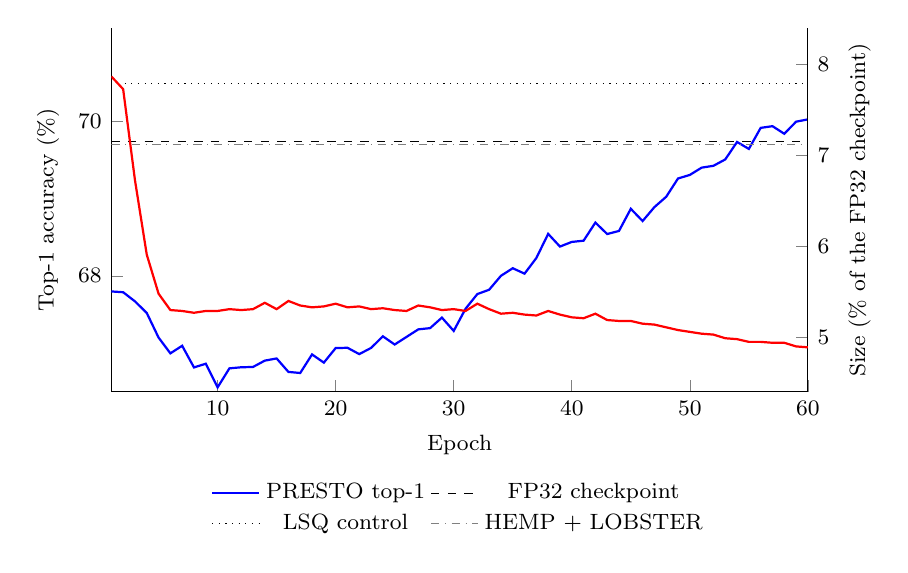
\begin{tikzpicture}
    \begin{axis}[
      width=0.86\textwidth, height=6.2cm,
      xlabel={Epoch}, xmin=1, xmax=60,
      ylabel={Top-1 accuracy (\%)}, ymin=66.5, ymax=71.2,
      axis y line*=left, axis x line*=bottom,
      legend style={at={(0.5,-0.22)}, anchor=north, legend columns=2, draw=none,
                    font=\footnotesize},
      tick label style={font=\footnotesize}, label style={font=\footnotesize},
    ]
      \addplot[thick, blue] coordinates {(1,67.798) (2,67.788) (3,67.670) (4,67.520) (5,67.202) (6,66.998) (7,67.096) (8,66.816) (9,66.864) (10,66.558) (11,66.804) (12,66.818) (13,66.822) (14,66.904) (15,66.932) (16,66.758) (17,66.744) (18,66.984) (19,66.878) (20,67.066) (21,67.070) (22,66.988) (23,67.068) (24,67.218) (25,67.112) (26,67.210) (27,67.308) (28,67.324) (29,67.460) (30,67.288) (31,67.574) (32,67.764) (33,67.820) (34,68.000) (35,68.098) (36,68.028) (37,68.230) (38,68.542) (39,68.378) (40,68.438) (41,68.454) (42,68.688) (43,68.540) (44,68.580) (45,68.866) (46,68.708) (47,68.888) (48,69.022) (49,69.258) (50,69.304) (51,69.398) (52,69.422) (53,69.504) (54,69.730) (55,69.640) (56,69.912) (57,69.934) (58,69.836) (59,69.992) (60,70.022)};
      \addlegendentry{PRESTO top-1}
      \addplot[dashed, black] coordinates {(1,69.734) (60,69.734)};
      \addlegendentry{FP32 checkpoint}
      \addplot[dotted, black] coordinates {(1,70.490) (60,70.490)};
      \addlegendentry{LSQ control}
      \addplot[dashdotted, gray] coordinates {(1,69.70) (60,69.70)};
      \addlegendentry{HEMP + LOBSTER}
    \end{axis}
    \begin{axis}[
      width=0.86\textwidth, height=6.2cm,
      xmin=1, xmax=60, ymin=4.4, ymax=8.4,
      ylabel={Size (\% of the FP32 checkpoint)},
      axis y line*=right, axis x line=none,
      tick label style={font=\footnotesize}, label style={font=\footnotesize},
    ]
      \addplot[thick, red] coordinates {(1,7.87) (2,7.73) (3,6.73) (4,5.91) (5,5.48) (6,5.30) (7,5.29) (8,5.27) (9,5.29) (10,5.29) (11,5.31) (12,5.30) (13,5.31) (14,5.38) (15,5.31) (16,5.40) (17,5.35) (18,5.33) (19,5.34) (20,5.37) (21,5.33) (22,5.34) (23,5.31) (24,5.32) (25,5.30) (26,5.29) (27,5.35) (28,5.33) (29,5.30) (30,5.31) (31,5.29) (32,5.37) (33,5.31) (34,5.26) (35,5.27) (36,5.25) (37,5.24) (38,5.29) (39,5.25) (40,5.22) (41,5.21) (42,5.26) (43,5.19) (44,5.18) (45,5.18) (46,5.15) (47,5.14) (48,5.11) (49,5.08) (50,5.06) (51,5.04) (52,5.03) (53,4.99) (54,4.98) (55,4.95) (56,4.95) (57,4.94) (58,4.94) (59,4.90) (60,4.89)};
    \end{axis}
  \end{tikzpicture}
  \caption{ResNet--18, the headline configuration
  $(T_1,T_2,T_3)=(10^{-5},10^{-7},6\times10^{-8})$ over sixty epochs. Blue, left
  axis: top-1 accuracy. Red, right axis: the serialized packet as a percentage of
  the FP32 checkpoint. The two phases are visible: the compression is delivered
  early, in the first ten epochs, while the accuracy recovers over the whole cosine
  and crosses the full-precision checkpoint at epoch fifty-four. The curve is one
  of the three repeats; it ends at $4.89\%$ of the checkpoint, which is also the
  mean of the three to the second decimal.
  Reference lines are the FP32
  checkpoint, the LSQ control at the same budget, and the closest published point.}
\end{figure}

\FloatBarrier

\section{Further Experimental Results}
\label{app:more-experiments}

This appendix reports the experiments that support Section~\ref{sec:experiments}
without being needed in order to follow it. Nothing here has been summarized, so
every number, every table and every caveat is given in full.
Figure~\ref{fig:frontier} places every run of the paper and every published point
within its range on a single panel.
\begin{figure}[t]
  \centering
  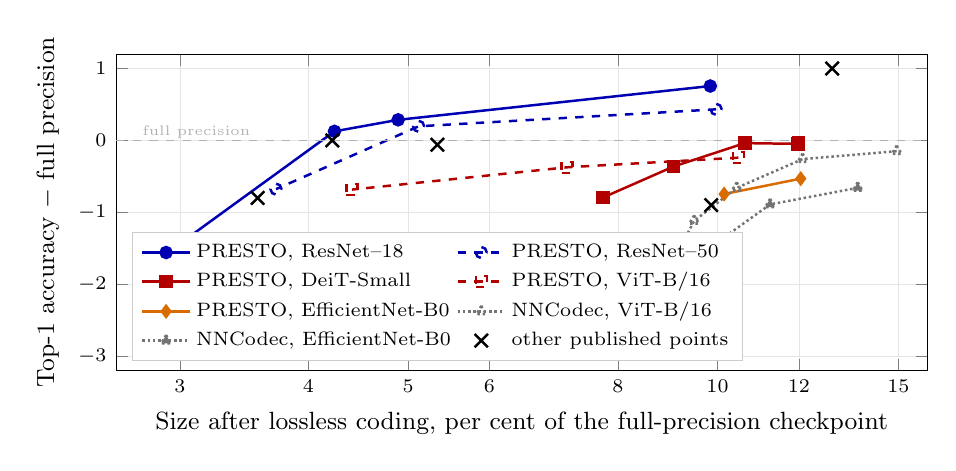
\begin{tikzpicture}
    \begin{axis}[
      width=0.98\textwidth, height=5.6cm,
      xlabel={Size after lossless coding, per cent of the full-precision checkpoint},
      ylabel={Top-1 accuracy $-$ full precision},
      xmode=log, log basis x=10,
      xtick={3,4,5,6,8,10,12,15}, xticklabels={3,4,5,6,8,10,12,15},
      xmin=2.6, xmax=16, ymin=-3.2, ymax=1.2,
      grid=both, grid style={line width=.2pt, draw=gray!20},
      legend style={font=\scriptsize, at={(0.02,0.03)}, anchor=south west,
                    legend columns=2, cells={anchor=west}, draw=gray!40},
      label style={font=\small}, tick label style={font=\scriptsize},
      every axis plot/.append style={line width=0.9pt, mark size=2pt},
      ]
      \addplot[color=blue!70!black, mark=*] coordinates
        {(9.84,0.756) (4.89,0.286) (4.24,0.126) (3.02,-1.404)};
      \addlegendentry{PRESTO, ResNet--18}
      \addplot[color=blue!70!black, dashed, mark=o] coordinates
        {(9.97,0.432) (5.12,0.196) (3.72,-0.678)};
      \addlegendentry{PRESTO, ResNet--50}
      \addplot[color=red!70!black, mark=square*] coordinates
        {(11.99,-0.036) (11.98,-0.048) (10.63,-0.038) (9.06,-0.364) (7.74,-0.794)};
      \addlegendentry{PRESTO, DeiT-Small}
      \addplot[color=red!70!black, dashed, mark=square] coordinates
        {(10.48,-0.240) (7.14,-0.374) (4.41,-0.684)};
      \addlegendentry{PRESTO, ViT-B/16}
      \addplot[color=orange!85!black, mark=diamond*] coordinates
        {(12.05,-0.532) (10.15,-0.746)};
      \addlegendentry{PRESTO, EfficientNet-B0}
      \addplot[color=black!55, mark=triangle, densely dotted] coordinates
        {(14.94,-0.15) (12.10,-0.26) (10.44,-0.66) (9.49,-1.12) (8.24,-2.81)};
      \addlegendentry{NNCodec, ViT-B/16}
      \addplot[color=black!55, mark=triangle*, densely dotted] coordinates
        {(13.69,-0.66) (11.25,-0.89) (10.08,-1.38) (9.03,-1.81)};
      \addlegendentry{NNCodec, EfficientNet-B0}
      \addplot[only marks, color=black, mark=x, mark size=3.4pt] coordinates
        {(4.22,0.0) (5.34,-0.06) (9.86,-0.9) (6.59,-2.39) (8.88,-1.61) (10.14,-1.62)
         (3.57,-0.8) (12.93,1.0)};
      \addlegendentry{other published points}
      \draw[gray!60, dashed] (axis cs:2.6,0) -- (axis cs:16,0);
      \node[font=\tiny, gray!60, anchor=west] at (axis cs:2.7,0.12) {full precision};
    \end{axis}
  \end{tikzpicture}
  \caption{Accuracy against size after lossless coding, as reported by each method
  for the checkpoint it uses. Accuracy is the difference from each method's own
  full-precision measurement, the only way to put five architectures on one panel;
  the raw accuracies behind every head-to-head claim are in
  Table~\ref{tab:main}. Crosses are single published points; LilNetX, at $2.16\%$
  and $-1.2$, falls to the left of the panel.}
  \label{fig:frontier}
\end{figure}

\subsection{Quantization-Aware Training Alone Makes Models Larger}
\label{sec:qat-fattens}

One measurement motivates the method before any comparison is made.
Table~\ref{tab:fatten} takes the LSQ-only control of every architecture and reads
its packet at the first epoch against its packet at the end, together with the
entropy of its non-zero symbols over the same interval.

\begin{table}[ht]
  \caption{Quantization-aware training on its own, with no regularizer, makes the
  quantized model \emph{harder} to compress while it gains accuracy. Four
  architectures, five controls, no exception. Sizes here are the packet over the
  FP32 bytes of the \emph{quantized tensors}, the accounting in which the relative
  change is read; over the whole checkpoint each row is larger by $1-f$, so the
  last ResNet--18 control reads $9.84\%$ in Table~\ref{tab:main}.}
  \label{tab:fatten}
  \centering \small
  \begin{tabular}{llccc}
    \toprule
    Control & Network, epochs & Packet, first $\to$ last & Change & $H$(non-zero) \\
    \midrule
    LSQ only & ResNet--18, 20 & $8.63\% \to 9.34\%$ & $+8.2\%$ & $2.796 \to 3.080$ \\
    LSQ only & ResNet--18, 60 & $8.59\% \to 9.76\%$ & $\mathbf{+13.6\%}$ & $2.788 \to 3.215$ \\
    LSQ only & ResNet--50, 20 & $8.83\% \to 9.78\%$ & $+10.8\%$ & $2.854 \to 3.147$ \\
    LSQ + distill. & DeiT-Small, 25 & $10.84\% \to 11.44\%$ & $+5.5\%$ & $3.352 \to 3.541$ \\
    LSQ + distill. & ViT-B/16, 20 & $9.67\% \to 10.19\%$ & $+5.4\%$ & $3.169 \to 3.316$ \\
    \bottomrule
  \end{tabular}
\end{table}

Sixty epochs of four-bit quantization-aware training on ResNet--18 gain $0.6$
accuracy points and at the same time make the serialized model $13.6\%$ larger,
while the entropy of the symbol histogram rises in every control that we ran, so
a low bit width clearly does not imply a low entropy and training left to itself
drifts in the wrong direction. Under the regularizer the same quantity falls by
between $0.468$ and $1.415$ bits across our runs, so PRESTO does not improve an
existing trend but reverses it.


\subsection{Budget Against Dose on ResNet--18}
\label{app:budget}

Budget, rather than dose, improves both axes at once. At $T_3=10^{-7}$ and sixty
epochs the run lands $0.128$ below the checkpoint, while the same configuration
at one hundred epochs reaches $0.126$ above it at the same packet and was still
gaining $0.03$ points per epoch when the schedule ended. Raising or lowering
$T_3$ trades one axis against the other, whereas lengthening the schedule does
not. The frontier does bend, and we report where: the marginal cost per point of size
is $0.625$ accuracy points between the sixty-epoch rows of
Tables~\ref{tab:main} and \ref{tab:extra} and $1.255$ between the two
hundred-epoch ones, the deeper of which is at $3.02\%$ and $1.404$ below.


\subsection{Joint Optimization Beats the Same Objective Decomposed}
\label{sec:pipeline}

PRESTO optimizes sparsity and code length together, whereas the obvious
alternative is to optimize them in sequence as the classical pipeline does, and
the question is whether the joint formulation earns the complexity that it adds.
We answer that question by decomposing our own objective rather than by comparing
against a different method, so that nothing except the ordering changes.

Two pipelines run twenty epochs on one term and then twenty on the other, in both
orders, starting from the same checkpoint and using the same coefficients as the
joint run. Each stage is a complete twenty-epoch cosine, identical in shape to the
joint reference, so the schedules are comparable stage by stage. The second stage
reloads the latent weights and re-initialises the step sizes by MSE, which is what
a sequential method does and is also, as we will see, part of the mechanism. The
only confound that remains is the budget, and it favours the pipeline, which
receives forty epochs against the twenty of the joint run, so we also report the
joint run at forty epochs, where the two are budget-matched.

\begin{table}[ht]
  \caption{Decomposing the objective, ResNet--18, $(T_1,T_2,T_3)=(10^{-5},10^{-7},
  3\cdot10^{-8})$ throughout. At matched budget the three accuracies agree to
  within $0.034$, well inside the $0.083$ spread between repeats, so the comparison is
  purely on size.}
  \label{tab:pipeline}
  \centering \small
  \begin{tabular}{lccc}
    \toprule
    Optimization & Epochs & Top-1 & Size \\
    \midrule
    Joint & 20 & 69.668 & 5.83\% \\
    \textbf{Joint} & \textbf{40} & \textbf{70.080} & $\mathbf{5.82\%}$ \\
    \addlinespace
    Sparsity alone, first stage & 20 & 70.098 & 7.46\% \\
    Sparsity then entropy & $20+20$ & 70.114 & 6.08\% \\
    \addlinespace
    Entropy alone, first stage & 20 & 69.782 & 6.09\% \\
    Entropy then sparsity & $20+20$ & 70.108 & 7.21\% \\
    \bottomrule
  \end{tabular}
\end{table}

At forty epochs the joint run is $4.3\%$ smaller than the better pipeline and
$19.4\%$ smaller than the worse one at the same accuracy, and the sharper way of
reading Table~\ref{tab:pipeline} is to ask what the second twenty epochs produce.
Against the joint run at twenty epochs, which is the common reference for all
three, every configuration ends between $0.41$ and $0.45$ accuracy points higher,
while the joint run holds its size to within $0.01$ points and the two pipelines
end $0.25$ and $1.39$ points larger. Read instead against each pipeline's own
first stage, which the table now reports, the asymmetry is starker: the entropy
stage of the first pipeline converts its twenty epochs into $1.38$ points of size
for $0.016$ of accuracy, whereas the sparsity stage of the second gives back
$1.12$ points of size for $0.326$ of accuracy. Sequential optimization therefore
spends the extra budget on accuracy that it can no longer spend on size.

The mechanism behind that behaviour is visible in the entropy of the non-zero
symbols. Re-quantizing between the two stages costs $0.343$ bits in one order and
$0.445$ bits in the other, because the grid is re-fitted to the latents that were
loaded and the symbols are remapped, and the entropy stage recovers that cost and
more, at $-0.742$ bits over its twenty epochs, whereas the sparsity stage cannot
recover it and adds a further $+0.040$. Running the entropy term first is
therefore self-defeating, because it gains $0.759$ bits, the re-fit gives back
$0.445$ of them and the sparsity stage then finishes $0.274$ bits above the point
at which the entropy stage began. Ordering matters, in the direction that the
classical pipeline happens to get right, and both orders lose to solving the two
problems together.


\subsection{Accuracy--Size Frontier on Vision Transformers}
\label{sec:transformers}

On both transformers the LSQ control does not clear the checkpoint the way the
ResNet controls do, so the object we report is the frontier against a
budget-matched control rather than a lossless claim. On ViT-B/16 five control
runs spanning learning rates from $3\times10^{-5}$ to $10^{-4}$ and budgets from
ten to thirty epochs land within a tenth of a point of each other and about two
tenths below full precision, from $-0.142$ to $-0.242$: there is no headroom to
spend, and no amount of budget creates any. Those five predate the packed-attention
fix of Appendix~\ref{app:configurations}, so only their accuracies are used
here and their sizes are not reported.

Against that control PRESTO removes $58\%$ of the ViT-B/16 packet for $0.444$
accuracy points, reaching $4.41\%$ of the checkpoint at $72.9\%$ sparsity, the
highest of any run here. On DeiT-Small the curve is traced by four doses along
the ray and the marginal cost rises monotonically: $0.001$, $0.208$ and $0.325$
accuracy points per point of packet, measured from the control through the half,
reference and double doses. The first of those is the interesting one,
because between the control and half the dose the packet falls from $11.99\%$ to
$10.63\%$ while the accuracy moves by $0.002$ points, which is far inside the
noise, so on this network the first $11\%$ of compression is free and the
trade-off only begins beyond that point.

A fifth dose deserves a separate mention, the fifth of the reference reported in
Table~\ref{tab:extra}, because there the sparsity rises from $13.7\%$ to $21.5\%$
and the packet does not move at all, from $11.99\%$ to $11.98\%$.
Below $50\%$ sparsity the support mask costs about $H(p)/32$ per weight and grows
faster than the symbol stream shrinks, so any sparsity gained there is paid for
twice, and the same arithmetic explains why our most compressed ResNet--18 rows
carry a cheaper mask than less sparse ones once they pass $p=1/2$.


\subsection{The Two Terms Act Through Different Mechanisms}
\label{sec:mechanism-ablation}

The sparsity and entropy terms are not two dials on a single mechanism. Measured
on the five matched ResNet--18 ablation arms of Appendix~\ref{app:ablation}, the
sparsity term contracts the latent distribution furthest, since its first
percentile moves $14.31\%$ towards zero against $11.66\%$ for the ridge alone,
and on EfficientNet-B0, where we also logged the step sizes
(Table~\ref{tab:mechanism}), it inflates them by $36\%$ while the control leaves
them unchanged, so widening the interval that maps to zero is the way in which it
creates sparsity. The entropy term leaves
both of those quantities where the ridge alone leaves them, at $11.25\%$ and
$\times 0.988$, and works on the assignment instead, cutting the value bytes by
$65\%$ against the sparsity term's $24\%$ and the entropy of the non-zero symbols
by $0.858$ bits, while the sparsity term moves that entropy by only $0.024$ and
the control lets it rise by $0.427$. The arms do not start from a common value,
$2.502$ bits under the sparsity term against $2.78$ elsewhere, because the first
measurement is taken at the end of the first epoch and the closed-form terms act
from the first optimizer step while the entropy term is still in its warm-up; the
quantity to compare is therefore the change along each run and not its endpoints.

The separation is therefore not pruning against coding. Both arms create zeros,
and on ResNet--18 the entropy term creates more of them, $60.30\%$ sparsity
against $45.56\%$, which follows from its minimizer at $c_b=1/e$ pushing mass into
the excluded zero symbol. What only one of the two does is shorten the code of the
weights that survive, and Section~\ref{sec:metaq-value} explains why we report
that as a measurement rather than as a property of the term.

\paragraph{Why they do not add.} Whichever term arrives first, the other has
little left to remove, and both ablations show it on the same quantity. On
AlexNet the two arms reach the same symbol distribution by different routes: the
entropy of the non-zero symbols starts at $2.892$ bits under the sparsity term
and $3.326$ under the entropy term, and \emph{both drive it to the same floor},
$1.688$ and $1.721$ bits, with the combination ending at $1.686$, which is
indistinguishable from sparsity alone. On ResNet--18 the floor is not shared,
because the sparsity term stops at $2.526$ bits while the entropy term reaches
$1.926$, and there the combination ends at $1.902$, which is indistinguishable
from entropy alone.
In both blocks the full objective lands on the floor of whichever single term
went lower, and the second term then contributes the few per cent of size
reported in Section~\ref{sec:term-ablation} rather than a second reduction. Which term gets
there first is the architecture-dependent quantity, and it is the same ordering
as the shares in Section~\ref{sec:term-ablation}.


\subsection{The AlexNet Deficit: What It Is Not, and What We Think It Is}
\label{app:alexnet-deficit}
 It is not the budget, since AlexNet has
converged at sixty epochs, the last ten gaining $0.010$ points per epoch on the
control and losing $0.004$ on the entropy arm. It is also not a healing phase too
short to recover from the pruning, the natural suspicion given how Deep
Compression is trained, because our sparse structure is $95\%$ final by epoch
$17$ to $20$ and leaves twenty-eight to thirty-one epochs above a tenth of the
base rate, against two on ResNet--18, where it settles only at epoch $46$.
AlexNet therefore gets an order of magnitude more high-rate retraining on its
final structure than the network that finishes above full precision, and the full
objective still ends $0.880$ below the checkpoint.

What we believe it is instead is allocation, and the arithmetic is worth writing
down even though we did not run the arm that would test it. Our sparsity is not
allocated: one coefficient pushes in the same way on eight tensors whose sizes
span three orders of magnitude, while both methods ahead of us assign a rate per
layer. The five convolutions hold $4.04\%$ of the weights, so pruning them at
$80\%$ gives $0.218$ points of packet, worth $0.021$ accuracy points at the
exchange rate we measure here and repaid by two extra points of sparsity on the
dense layers: we spend the feature extractor to save a fifth of a point that the
dense layers would return for almost nothing. This is a hypothesis and not a
measurement, and a per-layer dose is left to future work.


\subsection{Per-Channel Quantization Is Paid For Twice}
\label{sec:per-channel-twice}

Per-channel step sizes are usually treated as accuracy that comes for free. On
EfficientNet-B0, switching a matched control from per-channel to per-tensor cost
$0.098$ accuracy points and returned $1.03$ points of packet, which is a rate as
favourable as the one the sparsity term gives at its knee, and only $0.597$ of
that return was the metadata, a hard floor of one fp32 number per output channel
over $82$ tensors. The remaining $0.345$ came from the value stream, because one
shared grid per tensor gives the coder a single symbol distribution instead of
one distribution per output channel and the pooled stream is more concentrated.
Per-channel quantization therefore costs code length as well as metadata, and on
networks with many small tensors the two together are worth more than the
accuracy that it provides.


\subsection{Negative Results}
\label{sec:negative}

Four failures shaped the method and we report them because each changed what we
believed.

\textbf{The entropy coefficient is only as strong as its dual is converged.}
$T_3$ reaches the weights through one channel, the multiplier, and the dual range
to be crossed is proportional to $T_3$ while an absolute dual step is not.
Raising $T_3$ tenfold therefore left the applied gradient identical to four
significant figures and compressed \emph{less}, not more. The fix is to measure
the step as a fraction of the dual range; Appendix~\ref{app:dual-rate} derives the
rate. The general lesson is that when a coefficient looks inert, the dual
variable through which it acts should be checked for convergence before the
coefficient itself is touched.

\textbf{The dose cannot be derived, only measured and transported.} Three
analytic models for the sparsity coefficient failed in sequence, the first inert
by three orders of magnitude, the second divergent because it had been calibrated
on the wrong branch of the inner asymptotics, and the third overdosed tenfold
because the dominant channel was not present in the equation. What transfers between runs is the cumulative
exposure, the coefficient times the schedule sum, never the coefficient itself;
a ramp row reports the exposure accumulated up to that epoch and reproducing it
at fixed dose requires redoing the integral, a factor of $4.4$ in one case.

\textbf{A stopping criterion we wrote would have given the wrong answer.} We had
committed to abandoning the entropy channel on EfficientNet-B0 if it did not
separate from the control within four epochs at thirty times the reference dose.
It did not separate, but the cause was the dual rather than the dose, and the
channel opened as soon as the step was made relative.

\textbf{One diagnostic is worthless and we stopped using it.} The accuracy of the
network evaluated at its latent weights collapses by up to seventeen points
without predicting anything about the deployed model, because the straight-through
estimator applies a gradient computed at the quantized point to a latent that has
no restoring force toward it. The gap scales with the step size, not with the
regularizer, and it does not appear in this paper.
%----------------------------------------------------------------------------------------------------------
%----------------------------------------------------------------------------------------------------------
%----------------------------------------------------------------------------------------------------------
%----------------------------------------------------------------------------------------------------------
\section{Supplementary Derivations}
\label{app:derivations}
\label{app:supplementary}

\subsection{Learned-Step Quantization: Full Statement}
\label{app:lsq-details}
\label{sec:quantizer}

Let $Q_n<0<Q_p$ be two integers denoting the minimum and maximum integer codes,
respectively. The integer codebook is
\[
  \mathcal Q:=\{q\in\mathbb Z:Q_n\leq q\leq Q_p\},
  \qquad
  C:=|\mathcal Q|=Q_p-Q_n+1,
\]
where $\mathbb Z$ is the set of integers and $C$ is the number of symbols. We
associate each tensor $\ell$ with a quantization step size
$a_\ell\in\mathbb R_{>0}$. The collection of step sizes is
$a=\{a_\ell\}_{\ell\in\Lambda}$.

For $\alpha,\beta,u\in\mathbb R$ with $\alpha\leq\beta$, define
\[
  \operatorname{clip}(u;\alpha,\beta)
  :=\min\{\beta,\max\{\alpha,u\}\}.
\]
Moreover, let $\operatorname{round}(u)$ denote the integer nearest to $u$,
with ties resolved toward the even integer. For weight
$w_i^{(\ell)}$, we set
\begin{align}
  r_i^{(\ell)}
  &:=\frac{w_i^{(\ell)}}{a_\ell},
  \label{eq:normalized-weight}\\
  \bar w_i^{(\ell)}(a_\ell)
  &:=
  a_\ell\,
  \operatorname{clip}\!\left(
    r_i^{(\ell)};Q_n,Q_p
  \right),
  \label{eq:clipped-latent}\\
  \widehat w_i^{(\ell)}
  &:=
  a_\ell\,
  \operatorname{round}\!\left(
    \frac{\bar w_i^{(\ell)}(a_\ell)}{a_\ell}
  \right).
  \label{eq:quantizer}
\end{align}
$r_i^{(\ell)}$ is the weight normalized by the step size. The clipped latent
weight $\bar w_i^{(\ell)}(a_\ell)$ remains real-valued but is restricted to the
representable interval $[a_\ell Q_n,a_\ell Q_p]$. Rounding its normalized value
then produces $\widehat w_i^{(\ell)}$, which belongs to the real-valued codebook
$a_\ell\mathcal Q$ and is used in the forward pass.
The quantized weights of the entire network are
$\widehat w(a)=\{\widehat w^{(\ell)}\}_{\ell\in\Lambda}$.

PRESTO uses Learned Step Size Quantization (LSQ) \citep{esser2020lsq} to
propagate a surrogate gradient through the rounding operation. The PRESTO inner
problem operates on $\bar w_i^{(\ell)}$, ensuring that the quantizer and the
regularizer share the same representable domain.


%----------------------------------------------------------------------------------------------------
\subsection{Derivation of the Decomposed Dual}
\label{app:decomposition}

Fix a tensor $\ell\in\Lambda$, a clipped latent-weight vector
$\bar w^{(\ell)}$, and a step size $a_\ell$. For each count constraint, let
$\xi_b^{(\ell)}\in\mathbb R$ be an unrestricted Lagrange multiplier, and let
$\xi^{(\ell)}=(\xi_b^{(\ell)})_{b\in\mathcal B}$ collect these multipliers. 
For the Lagrangian relaxation of each count constraint, we use the sign convention
\[
  \xi_b^{(\ell)}
  \left(
    \sum_{i\in\mathcal I_\ell}x_{i,b}^{(\ell)}-c_b^{(\ell)}
  \right).
\]
The partial Lagrangian of tensor $\ell$, obtained by dualizing only the count constraints, is
\begin{align}
 \mathscr L_\ell(x^{(\ell)},y^{(\ell)},c^{(\ell)};
                  \xi^{(\ell)})
 :=\;&
 T_1\sum_{i\in\mathcal I_\ell}
      \frac{(\bar w_i^{(\ell)})^2}{y_i^{(\ell)}}
 +T_2\sum_{i\in\mathcal I_\ell}y_i^{(\ell)}
 \notag\\
 &+T_3\sum_{b\in\mathcal B}
      c_b^{(\ell)}\log_2 c_b^{(\ell)}
 +\sum_{b\in\mathcal B}\xi_b^{(\ell)}
   \left(
     \sum_{i\in\mathcal I_\ell}x_{i,b}^{(\ell)}-c_b^{(\ell)}
   \right).
 \label{eq:partial-lagrangian}
\end{align}
The variables $x^{(\ell)}$ and $y^{(\ell)}$ retain the domain constraints in
Eq.~\eqref{eq:domain} and the representation and mass constraints in
Eqs.~\eqref{eq:representation} and \eqref{eq:mass}, while
$c_b^{(\ell)}\geq 0$ for every $b\in\mathcal B$. The count constraints
themselves are no longer imposed explicitly, because their violation is priced
by $\xi^{(\ell)}$.

Let $\varphi_{\bar w^{(\ell)},a_\ell}^{(\ell)}(\xi^{(\ell)})$ denote the minimum of
$\mathscr L_\ell$ over these remaining feasible variables. The function
$\varphi_{\bar w^{(\ell)},a_\ell}^{(\ell)}$ is the Lagrangian dual function and is concave in
$\xi^{(\ell)}$, because it is the pointwise infimum of affine functions of the
multipliers. Rearranging Eq.~\eqref{eq:partial-lagrangian} yields
\begin{align}
 \varphi_{\bar w^{(\ell)},a_\ell}^{(\ell)}(\xi^{(\ell)})
 :={}&
 \min_{\substack{
       (x_i^{(\ell)},y_i^{(\ell)})\in\mathcal F_i^{(\ell)}
       \ \forall i\in\mathcal I_\ell,\\
       c_b^{(\ell)}\geq0\ \forall b\in\mathcal B}}
 \mathscr L_\ell
 \bigl(x^{(\ell)},y^{(\ell)},c^{(\ell)};\xi^{(\ell)}\bigr)
 \notag\\
 ={}&
 \sum_{b\in\mathcal B}
 \min_{c_b^{(\ell)}\geq0}
 \left\{
   T_3c_b^{(\ell)}\log_2c_b^{(\ell)}
   -\xi_b^{(\ell)}c_b^{(\ell)}
 \right\}
 \notag\\
 &+\sum_{i\in\mathcal I_\ell}
 \min_{(x_i^{(\ell)},y_i^{(\ell)})\in
       \mathcal F_i^{(\ell)}}
 \left\{
   T_1\frac{(\bar w_i^{(\ell)})^2}{y_i^{(\ell)}}
   +T_2y_i^{(\ell)}
   +\sum_{b\in\mathcal B}
      \xi_b^{(\ell)}x_{i,b}^{(\ell)}
 \right\},
\end{align}


%----------------------------------------------------------------------------------------------------
\subsection{Solving the Per-Weight Subproblem}
\label{app:subproblem}
\label{app:per-weight-derivation}


Fix a tensor $\ell\in\Lambda$. Throughout this section, we temporarily omit
the superscript $(\ell)$, with the understanding that all quantities refer to
the same tensor. Accordingly, $\xi=(\xi_b)_{b\in\mathcal B}$ denotes the
multiplier vector introduced in Section~\ref{sec:lagrangian-decomposition}
with its tensor superscript omitted.

For fixed $\xi$, the problem separates over the weight index $i$. Given a
weight $\bar w_i$ and a fixed mass $y_i\in[0,1]$, define
\begin{align}
 K_i(y_i;\bar w_i,\xi,v)
 :=\min_{x_i}\quad&
 \sum_{b\in\mathcal B}\xi_bx_{i,b}
 \label{eq:knapsack-objective}\\
 \text{s.t.}\quad&
 \left\{
 \begin{aligned}
  \sum_{b\in\mathcal B}v_bx_{i,b}&=\bar w_i,
  &\qquad \sum_{b\in\mathcal B}x_{i,b}&=y_i,\\
  x_{i,b}&\geq0,
  && b\in\mathcal B.
 \end{aligned}
 \right.
 \label{eq:knapsack-constraints}
\end{align}
The letter $K$ denotes the optimal value of this linear knapsack-type
subproblem, and the subscript $i$ identifies the corresponding weight. Here,
$x_i=(x_{i,b})_{b\in\mathcal B}$ is the vector of assignment masses for weight
$i$, and $v=(v_b)_{b\in\mathcal B}$ is the vector of real-valued levels.

For $y_i>0$, let
\[
  u_{i,b}:=\frac{x_{i,b}}{y_i},
  \qquad
  \widetilde w_i:=\frac{\bar w_i}{y_i}.
\]
The vector $u_i=(u_{i,b})_{b\in\mathcal B}$ has nonnegative entries summing to
one, while $\widetilde w_i$ is the rescaled target. It follows that
\begin{equation}
  K_i(y_i;\bar w_i,\xi,v)
  =
  y_i\,K_i(1;\widetilde w_i,\xi,v).
  \label{eq:perspective-scaling}
\end{equation}

To evaluate $K_i(1;\widetilde w_i,\xi,v)$, we associate each symbol $b$ with the
point $P_b:=(v_b,\xi_b)\in\mathbb R^2$. The optimal value is the ordinate of
the lower convex hull of the points $P_b$ at the abscissa
$v=\widetilde w_i$. Let~$E_{\mathrm l}$ and $E_{\mathrm r}$ denote,
respectively, the leftmost and rightmost vertices of the lower hull, as shown
in Figure~\ref{fig:lower-hull}. Suppose first that
$v_{b_-}<\widetilde w_i<v_{b_+}$, where $P_{b_-}$ and $P_{b_+}$ are the
endpoints of the lower-hull facet containing this abscissa. We call these
points active because they determine the facet and are the only symbols assigned
positive mass in the corresponding two-point optimal representation. 
If $\widetilde w_i$ coincides with a lower-hull
vertex $v_b$, the optimal representation assigns unit mass to symbol $b$.
If $P_b$ is an interior vertex of the lower hull, either of its two incident
facets may be used in the formulas below. If $P_b$ is one of the two extreme
vertices $E_{\mathrm l}$ and $E_{\mathrm r}$, only one incident facet exists.
In both cases, the formulas yield unit mass for symbol $b$ and zero mass for
the other vertex of the selected facet.

\begin{figure}[ht]
\centering
\begin{tikzpicture}[scale=1.15,>=latex]
  \draw[->] (-2.6,0) -- (3.9,0) node[right] {$v$};
  \draw[->] (0,-0.15) -- (0,4.7) node[above] {$\xi$};
  \node[below left] at (0,0) {\small $0$};

  \coordinate (A) at (-2.2,3.2);
  \coordinate (B) at (-1.0,1.4);
  \coordinate (C) at (0.4,0.6);
  \coordinate (D) at (1.6,1.0);
  \coordinate (E) at (2.6,2.6);
  \coordinate (F) at (3.4,4.2);

  \draw[gray!65,dashed] (A)--(B)--(C)--(D)--(E)--(F);
  \foreach \p in {A,B,E,F} \fill[gray!70] (\p) circle (1.7pt);
  \node[above left] at (A) {\small $E_{\mathrm l}$};
  \node[above right] at (F) {\small $E_{\mathrm r}$};
  \draw[very thick] (C)--(D);
  \fill (C) circle (2.2pt);
  \fill (D) circle (2.2pt);
  \node[below right] at (C) {\small $P_{b_-}$};
  \node[above right] at (D) {\small $P_{b_+}$};

  \draw[thin,dashed] (0,0.4667)--(C);
  \fill (0,0.4667) circle (1.9pt);
  \node[left] at (0,0.4667) {\small $s_i$};

  \draw[dotted] (1.1,0)--(1.1,0.83);
  \fill (1.1,0.83) circle (1.7pt);
  \node[below] at (1.1,0) {\small $\widetilde w_i$};
  \node[right] at (1.05,0.70)
    {\small $K_i(1;\widetilde w_i,\xi,v)$};
  %\node[above left] at (1.30,0.93) {\small slope $\mu_i$};
\end{tikzpicture}
\caption{Geometric solution of the normalized per-weight subproblem.}
\label{fig:lower-hull}
\end{figure}

Consider the two-point optimal representation associated with the selected
facet. All masses outside its endpoints are set to zero, while the endpoint
masses satisfy
\[
  u_{i,b_-}+u_{i,b_+}=1,
  \qquad
  v_{b_-}u_{i,b_-}+v_{b_+}u_{i,b_+}=\widetilde w_i.
\]
Solving this two-equation linear system yields
\begin{align}
  u_{i,b_-}
  &=
  \frac{v_{b_+}-\widetilde w_i}{v_{b_+}-v_{b_-}},
  &
  u_{i,b_+}
  &=
  \frac{\widetilde w_i-v_{b_-}}{v_{b_+}-v_{b_-}}.
  \label{eq:active-masses}
\end{align}
Both masses are strictly positive when $\widetilde w_i$ lies in the interior
of the facet; if it coincides with an endpoint, the corresponding masses are
$1$ and $0$.

The line containing the active facet can be written as
$\xi=\mu_i v+s_i$. Requiring this line to pass through $P_{b_-}$ and
$P_{b_+}$ yields
\begin{align}
  \mu_i
  &:=
  \frac{\xi_{b_+}-\xi_{b_-}}{v_{b_+}-v_{b_-}},
  &
  s_i
  &:=
  \frac{\xi_{b_-}v_{b_+}-\xi_{b_+}v_{b_-}}
       {v_{b_+}-v_{b_-}}.
  \label{eq:slope-intercept}
\end{align}
Therefore,
\begin{equation}
  K_i(1;\widetilde w_i,\xi,v)
  =\mu_i\widetilde w_i+s_i.
  \label{eq:lower-hull}
\end{equation}

\paragraph{Breakpoints of the active facet.}
The facet that supports $\widetilde w_i=\bar w_i/y_i$ changes only when
$\widetilde w_i$ crosses a vertex of the lower hull. Let
$v_{(1)},\dots,v_{(m)}$ be the abscissas of the hull vertices that have the
same sign as $\bar w_i$, sorted by increasing magnitude. As $y_i$ decreases
from $1$ to $y_i^{\min}$, the ratio $|\widetilde w_i|=|\bar w_i|/y_i$ increases
monotonically from $|\bar w_i|$ to $V_i^{\max}$. The active facet therefore
changes exactly at
\begin{equation}
  y_{(k)}
  :=
  \frac{|\bar w_i|}{|v_{(k)}|},
  \qquad
  y_{(k)}\in[y_i^{\min},1],
  \label{eq:app-breakpoints}
\end{equation}
and these values, together with $y_i^{\min}$ and $1$, partition the feasible
interval into at most $m\leq C$ subintervals. The pair $(\mu_i,s_i)$ is
constant on each subinterval, so Eq.~\eqref{eq:app-y-candidate} applies there
unchanged. The breakpoints require no search: they are obtained in closed form
from the hull vertices, which are shared by every weight of the tensor.

\paragraph{Cost of the comparison.}
The lower hull of the $C$ points $(v_b,\xi_b)$ does not depend on $i$. It is
built once per tensor and per dual iteration, in $O(C)$ time by a monotone
chain, because the codebook values are already sorted. For a single weight, the
initial facet is located by binary search in $O(\log C)$; the sweep then visits
at most $m\leq C$ subintervals and performs constant work in each, namely one
evaluation of Eq.~\eqref{eq:app-y-candidate}, one clipping test, and one evaluation
of $G_i$. The per-weight cost is therefore $O(C)$ in the worst case and
$O(\log C)$ when the feasible interval spans few facets. One pass over a tensor
with $n_\ell$ weights costs $O(C+n_\ell C)$, and a dual update with
$N_{\mathrm{dual}}$ iterations costs $N_{\mathrm{dual}}$ such passes. Since $C$
is a small constant (16 in all our experiments) and the sweep is vectorized
over weights, the measured cost of the solver is a small multiple of one
elementwise pass over the tensor; Section~\ref{sec:experiments} reports the
wall-clock effect.

To characterize the feasible interval of $y_i$, define
\[
  V_i^{\max}
  :=
  \max\{|v_b|:b\in\mathcal B,\ \bar w_i v_b\geq0\}.
\]
If $\bar w_i=0$, define $y_i^{\min}:=0$; otherwise, define
\[
  y_i^{\min}:=\frac{|\bar w_i|}{V_i^{\max}}.
\]
$V_i^{\max}$ is the largest representable magnitude having the same sign as
$\bar w_i$, whereas $y_i^{\min}$ is the smallest mass that can represent
$\bar w_i$.

It remains to minimize the scalar function
\begin{equation}
  G_i(y_i)
  :=
  K_i(y_i;\bar w_i,\xi,v)
  +T_1\frac{\bar w_i^2}{y_i}
  +T_2y_i,
  \qquad
  y_i\in[y_i^{\min},1],
  \label{eq:app-scalar-problem}
\end{equation}
where $G_i$ is the value of the subproblem associated with weight $i$. On an
interval over which the active facet remains unchanged,
$K_i(y_i;\bar w_i,\xi,v)=\mu_i\bar w_i+s_i y_i$. If $s_i+T_2>0$, the unique
stationary candidate in the interior of that interval is
\begin{equation}
  y_i^{\mathrm{cand}}
  :=
  |\bar w_i|
  \sqrt{\frac{T_1}{s_i+T_2}}.
  \label{eq:app-y-candidate}
\end{equation}
Here, $s_i$ is not an optimized quantity. For each candidate interval, it is
computed from the lower-hull facet that remains active throughout that
interval, using Eq.~\eqref{eq:slope-intercept}, before
$y_i^{\mathrm{cand}}$ is evaluated. The candidates obtained from all active
facets are compared only afterward to select $y_i^*$. 
The algorithm compares every candidate $y_i^{\mathrm{cand}}$ lying within its
corresponding interval against the interval endpoints and the endpoints of
$[y_i^{\min},1]$. We denote the resulting minimizer by $y_i^*$. The optimal
mass assigned to the zero symbol is $z_i^*:=1-y_i^*$.

\paragraph{The zero weight.} One case has to be singled out. If $\bar w_i=0$ then
$y_i^{\min}=0$, the whole feasible interval is available and, whenever the active
prices are non-negative, the minimizer is $y_i^*=0$ with $x_i=0$, so the
expression $\mu_i+2T_1\bar w_i/y_i^*$ of Eq.~\eqref{eq:beta-star} is $0/0$ and
does not define a value. It is a genuine kink rather than an artefact: along the
stationary branch $y_i=|\bar w_i|\sqrt{T_1/(s_i+T_2)}$ the perspective part tends
to $\pm2\sqrt{T_1(s_i+T_2)}$ as $\bar w_i\to0^{\pm}$, so the two one-sided limits
bracket the origin and the subdifferential of $G_i^*$ at $\bar w_i=0$ is an
interval containing zero. The implementation selects $\beta_i^*=0$ there, the
midpoint of that interval, and Algorithm~\ref{alg:hull} states the branch
explicitly.


%----------------------------------------------------------------------------------------------------
\subsection{Regularizer Subgradient with Respect to the Weights}
\label{app:weight-grad}
\label{app:weight-gradient}
\label{sec:regularizer-weight-subgradient}

Restoring the tensor superscript $\ell$, let $\mu_i^{(\ell)}$ be an optimal
Lagrange multiplier associated with the representation constraint of
Eq.~\eqref{eq:representation} for weight $i$, under the sign convention
\[
  \bar w_i^{(\ell)}
  -\sum_{b\in\mathcal B}
   a_\ell q_bx_{i,b}^{(\ell)}
  =0.
\]
The full inner Lagrangian, obtained by adding the representation constraints
to the partial Lagrangian in Eq.~\eqref{eq:partial-lagrangian}, is
\[
  \mathscr L_\ell^{\mathrm{full}}
  :=
  \mathscr L_\ell
  +
  \sum_{i\in\mathcal I_\ell}
  \mu_i^{(\ell)}
  \left(
    \bar w_i^{(\ell)}
    -
    \sum_{b\in\mathcal B}
    a_\ell q_bx_{i,b}^{(\ell)}
  \right).
\]
For a convex parametric optimization problem the optimal Lagrange multipliers
describe how the optimal-value function responds to perturbations of the
constraints, and when the parameter also appears explicitly in the objective its
direct contribution has to be added to the contribution of the multiplier
\citep{bonnans2000perturbation}.

The connection with the per-weight function $G_i$ in
Eq.~\eqref{eq:app-scalar-problem} can be seen directly. Temporarily omitting the
tensor superscript, Eqs.~\eqref{eq:perspective-scaling} and
\eqref{eq:lower-hull} give, on the selected facet,
\[
  K_i(y_i;\bar w_i,\xi,v)
  =
  \mu_i\bar w_i+s_i y_i.
\]
Consequently,
\[
  \mu_i
  \in
  \partial_{\bar w_i}
  K_i(y_i;\bar w_i,\xi,v),
\]
where the inclusion accounts for a possible lower-hull breakpoint. From Eq.~\eqref{eq:app-scalar-problem}
we obtain, for fixed $y_i$,
\[
  \mu_i+2T_1\frac{\bar w_i}{y_i}
  \in
  \partial_{\bar w_i}G_i(y_i).
\]

To make the minimization over $y_i$ explicit, define the optimized per-weight
value
\[
  G_i^*(\bar w_i;\xi,v)
  :=
  \min_{y_i\in[y_i^{\min},1]}
  G_i(y_i;\bar w_i,\xi,v),
  \qquad
  y_i^*\in\arg\min_{y_i\in[y_i^{\min},1]}
  G_i(y_i;\bar w_i,\xi,v),
\]
In this notation $G_i^*$ denotes the optimal value while $y_i^*$ denotes a
selected minimizer.
The dependence of $G_i$ on $\bar w_i$, $\xi$, and $v$ was suppressed in
Eq.~\eqref{eq:app-scalar-problem}. At a differentiability point where $y_i^*$ is
an interior minimizer, formally applying the chain rule to
$G_i^*(\bar w_i;\xi,v)=G_i(y_i^*(\bar w_i);\bar w_i,\xi,v)$ gives
\[
  \frac{dG_i^*}{d\bar w_i}
  =
  \frac{\partial G_i}{\partial\bar w_i}
  +
  \frac{\partial G_i}{\partial y_i}
  \frac{dy_i^*}{d\bar w_i}
  =
  \frac{\partial G_i}{\partial\bar w_i},
\]
because $\left.\frac{\partial G_i}{\partial y_i}\right|_{y_i=y_i^*}=0$
at the interior optimum. Danskin's
theorem and the sensitivity theory of convex value functions extend this
conclusion to lower-hull breakpoints and boundary minimizers: a compatible
subgradient is obtained from a selected optimal primal--dual solution while
holding $y_i^*$ fixed \citep{danskin1966maxmin,bonnans2000perturbation}.
Therefore, no derivative of $y_i^*$ is required, and
\[
  \mu_i+2T_1\frac{\bar w_i}{y_i^*}
  \in
  \partial_{\bar w_i}G_i^*(\bar w_i;\xi,v).
\]

Restoring the tensor superscript, and observing that the count subproblems
contain no explicit dependence on $\bar w_i^{(\ell)}$, yields
\begin{equation}
  \beta_i^{(\ell)*}
  :=
  \mu_i^{(\ell)}
  +2T_1
   \frac{\bar w_i^{(\ell)}}{y_i^{(\ell)*}}
  \in
  \left.
  \partial_{\bar w_i^{(\ell)}}
  \Phi_\ell\!\left(\bar w^{(\ell)},a_\ell\right)
  \right|_{a_\ell}.
  \label{eq:app-weight-envelope}
\end{equation}
Thus, $\mu_i^{(\ell)}$ is the contribution induced by the representation
constraint, whereas the second term is the direct contribution of the perspective
penalty. Everything in this subsection and the next is written at a dual optimum,
where $\varphi^{(\ell)}$ and $\Phi_\ell$ coincide; the implementation evaluates the
same expressions at the multiplier it currently holds, and
Appendix~\ref{app:boundary-kkt-derivation} states what they are exact for in that
case. If $\Phi_\ell$ is differentiable with respect to $\bar w_i^{(\ell)}$, the
subgradient is unique and
\[
  \beta_i^{(\ell)*}
  =
  \left.
  \frac{\partial\Phi_\ell}
       {\partial\bar w_i^{(\ell)}}
  \right|_{a_\ell}.
\]

At points where the active facet changes, $\Phi_\ell$ may be nondifferentiable;
the preceding quantities should then be interpreted as subgradients 
associated with either adjacent active facet. 
If the optimal normalized value reaches the extreme level
$v_e^{(\ell)}$, namely
$\bar w_i^{(\ell)}/y_i^{(\ell)*}=v_e^{(\ell)}$, representability forces all
nonzero mass onto the corresponding extreme symbol $e\in\mathcal B$. The KKT
conditions then yield
\begin{equation}
  \mu_i^{(\ell)}
  =
  \frac{\xi_e^{(\ell)}+T_2}{v_e^{(\ell)}}
  -T_1v_e^{(\ell)}.
  \label{eq:boundary-kkt}
\end{equation}
when $y_i^{(\ell)*}=y_i^{(\ell),\min}<1$. If the weight itself coincides with
the extreme level, so that $y_i^{(\ell)*}=1$, Eq.~\eqref{eq:boundary-kkt}
selects the limiting multiplier obtained by approaching the endpoint from the
interior of the representable interval. Here, $\xi_e^{(\ell)}$ is the dual
multiplier associated with the count-defining constraint for symbol $e$ in
Eq.~\eqref{eq:counts}. Appendix~\ref{app:boundary-kkt-derivation} derives
Eq.~\eqref{eq:boundary-kkt} and explains the endpoint selection.


%----------------------------------------------------------------------------------------------------
\subsection{Regularizer Gradient with Respect to the Step Sizes}
\label{app:scale-grad}
\label{app:scale-gradient}
\label{sec:regularizer-step-gradient}

Holding $\bar w^{(\ell)}$ fixed, the step size $a_\ell$ appears explicitly in
the full inner Lagrangian $\mathscr L_\ell^{\mathrm{full}}$ only through the
representation-constraint term
\[
  -\sum_{i\in\mathcal I_\ell}
   \mu_i^{(\ell)}
   \sum_{b\in\mathcal B}
   a_\ell q_bx_{i,b}^{(\ell)},
\]
because $v_b^{(\ell)}(a_\ell)=a_\ell q_b$. The envelope theorem therefore
computes the derivative of the optimal-value function by differentiating this
explicit dependence at an optimal primal--dual solution; derivatives of the
optimal assignments $x_{i,b}^{(\ell)*}$ with respect to $a_\ell$ are not
required \citep{bonnans2000perturbation}. Since
$\partial v_b^{(\ell)}/\partial a_\ell=q_b$, this gives
\begin{equation}
  \left.
  \frac{\partial\Phi_\ell}{\partial a_\ell}
  \right|_{\bar w^{(\ell)}}
  =
  -\sum_{i\in\mathcal I_\ell}
   \mu_i^{(\ell)}
   \sum_{b\in\mathcal B}
   q_bx_{i,b}^{(\ell)*}
  =
  -\frac{1}{a_\ell}
   \sum_{i\in\mathcal I_\ell}
   \mu_i^{(\ell)}\bar w_i^{(\ell)}.
  \label{eq:app-scale-envelope}
\end{equation}
Thus, the first equality follows from the envelope theorem. The second follows
from the representation constraint in Eq.~\eqref{eq:representation}, together
with $v_b^{(\ell)}=a_\ell q_b$.


%----------------------------------------------------------------------------------------------------
\subsection{KKT Multiplier at a Representability Boundary}
\label{app:boundary-kkt-derivation}

Here we derive the representation multiplier reported in
Eq.~\eqref{eq:boundary-kkt}. Fix a tensor $\ell$ and a weight
$i\in\mathcal I_\ell$, and suppose that its optimal mass attains the
representability lower bound
\[
  y_i^{(\ell)*}
  =y_i^{(\ell),\min}
  =\frac{|\bar w_i^{(\ell)}|}{|v_e^{(\ell)}|},
\]
where $v_e^{(\ell)}$ is the extreme codebook level having the same sign as
$\bar w_i^{(\ell)}$. Equivalently,
\[
  \frac{\bar w_i^{(\ell)}}{y_i^{(\ell)*}}
  =v_e^{(\ell)}.
\]
Because no codebook level extends beyond $v_e^{(\ell)}$ in that direction, the
representation and mass constraints can hold only if all nonzero mass is
assigned to symbol $e$:
\[
  x_{i,e}^{(\ell)*}=y_i^{(\ell)*},
  \qquad
  x_{i,b}^{(\ell)*}=0
  \quad\text{for every }b\neq e.
\]

Let $\rho_i^{(\ell)}\in\mathbb R$ be the Lagrange multiplier associated with
the mass constraint
\[
  \sum_{b\in\mathcal B}x_{i,b}^{(\ell)}-y_i^{(\ell)}=0.
\]
For every $b\in\mathcal B$, let $\gamma_{i,b}^{(\ell)}\geq0$ be the multiplier
associated with the nonnegativity constraint written as
$-x_{i,b}^{(\ell)}\leq0$.
Using for the representation constraint the sign convention introduced in
Appendix~\ref{sec:regularizer-weight-subgradient}, define the per-weight KKT
Lagrangian relevant to the derivation as
\begin{align*}
  \mathscr L_{i,\ell}^{\mathrm{KKT}}
  :={}&T_1\frac{(\bar w_i^{(\ell)})^2}{y_i^{(\ell)}}
  +T_2y_i^{(\ell)}
  +\sum_{b\in\mathcal B}\xi_b^{(\ell)}x_{i,b}^{(\ell)} \\
  &\quad
  +\mu_i^{(\ell)}
   \left(
     \bar w_i^{(\ell)}
     -\sum_{b\in\mathcal B}v_b^{(\ell)}x_{i,b}^{(\ell)}
   \right)
  +\rho_i^{(\ell)}
   \left(
     \sum_{b\in\mathcal B}x_{i,b}^{(\ell)}-y_i^{(\ell)}
   \right)
  -\sum_{b\in\mathcal B}\gamma_{i,b}^{(\ell)}x_{i,b}^{(\ell)}.
\end{align*}
Complementary slackness requires
$\gamma_{i,e}^{(\ell)}x_{i,e}^{(\ell)*}=0$; since
$x_{i,e}^{(\ell)*}>0$, it follows that
$\gamma_{i,e}^{(\ell)}=0$.\footnote{For an inequality written as
$-x_{i,e}^{(\ell)}\leq0$, the KKT complementary-slackness condition is
$\gamma_{i,e}^{(\ell)}x_{i,e}^{(\ell)*}=0$. Thus, strict positivity of the
primal variable forces the associated nonnegativity multiplier to vanish; see
\citet{bonnans2000perturbation}.} Stationarity with respect to the active mass,
evaluated at the selected optimum, therefore gives
\begin{equation}
  \left.
  \frac{\partial\mathscr L_{i,\ell}^{\mathrm{KKT}}}
       {\partial x_{i,e}^{(\ell)}}
  \right|_{\substack{x_i^{(\ell)}=x_i^{(\ell)*}\\
                     y_i^{(\ell)}=y_i^{(\ell)*}}}
  =\xi_e^{(\ell)}
  -\mu_i^{(\ell)}v_e^{(\ell)}
  +\rho_i^{(\ell)}
  -\gamma_{i,e}^{(\ell)}
  =\xi_e^{(\ell)}
  -\mu_i^{(\ell)}v_e^{(\ell)}
  +\rho_i^{(\ell)}
  =0.
  \label{eq:boundary-kkt-x-stationarity}
\end{equation}
When $y_i^{(\ell)*}<1$, the upper bound $y_i^{(\ell)}\leq1$ is inactive.
Stationarity with respect to $y_i^{(\ell)}$ then yields
\begin{equation}
  -T_1
   \frac{(\bar w_i^{(\ell)})^2}{(y_i^{(\ell)*})^2}
  +T_2
  -\rho_i^{(\ell)}
  =0.
  \label{eq:boundary-kkt-y-stationarity}
\end{equation}
Using
$\bar w_i^{(\ell)}/y_i^{(\ell)*}=v_e^{(\ell)}$ in
Eq.~\eqref{eq:boundary-kkt-y-stationarity} gives
\[
  \rho_i^{(\ell)}
  =T_2-T_1(v_e^{(\ell)})^2.
\]
Substitution into Eq.~\eqref{eq:boundary-kkt-x-stationarity} produces
\[
  \mu_i^{(\ell)}
  =
  \frac{\xi_e^{(\ell)}+T_2}{v_e^{(\ell)}}
  -T_1v_e^{(\ell)},
\]
which is Eq.~\eqref{eq:boundary-kkt}.

The endpoint case remains to be clarified. If
$\bar w_i^{(\ell)}=v_e^{(\ell)}$, then representability forces
$y_i^{(\ell)*}=1$ and the upper-bound multiplier for $y_i^{(\ell)}\leq1$ may be
nonzero, so that the representation multiplier is not necessarily unique, and in
that situation Equation~\eqref{eq:boundary-kkt} specifies the multiplier
obtained by setting that upper-bound multiplier to zero, equivalently the limit
of the preceding expression as $\bar w_i^{(\ell)}$ approaches
$v_e^{(\ell)}$ from the interior of the representable interval. This is the
subgradient selection used in the optimization procedure.


%----------------------------------------------------------------------------------------------------
\subsection{Count Solutions and Dual Residuals}
\label{app:count-solutions}

Fix a tensor $\ell\in\Lambda$ and a multiplier vector $\xi^{(\ell)}$. For each
symbol $b\in\mathcal B$, the solutions of the per-weight subproblems determine
the reconstructed count
\begin{equation}
  \widehat c_b^{(\ell)}
  :=
  \sum_{i\in\mathcal I_\ell}x_{i,b}^{(\ell)*}.
  \label{eq:app-reconstructed-count}
\end{equation}
The hat distinguishes this quantity, which is reconstructed by summing the
optimal assignment masses, from the independent variable $c_b^{(\ell)}$ in
the count subproblem.

For $T_3>0$, the count subproblem appearing in the first line of
Eq.~\eqref{eq:dual-decomposition} is
\[
  \min_{c_b^{(\ell)}\geq0}
  \left\{
    T_3c_b^{(\ell)}\log_2c_b^{(\ell)}
    -\xi_b^{(\ell)}c_b^{(\ell)}
  \right\}.
\]
Its objective is strictly convex for $c_b^{(\ell)}>0$ and its derivative on this interval is
\[
  \frac{T_3}{\ln(2)}\bigl(\ln c_b^{(\ell)}+1\bigr)
  -\xi_b^{(\ell)}.
\]
Setting this derivative to zero and solving for $c_b^{(\ell)}$ gives the
unconstrained stationary value
\begin{equation}
  c_{b,\mathrm{unc}}^{(\ell)}
  =
  \exp\!\left(
    \frac{\ln(2)\,\xi_b^{(\ell)}}{T_3}-1
  \right).
  \label{eq:app-unconstrained-count-solution}
\end{equation}
For numerical stability, the implementation restricts the count to
$[c_{\min},n_\ell]$, where $c_{\min}>0$ is a fixed numerical lower bound and
$n_\ell$ is the number of weights in tensor $\ell$. The value actually used by
the dual solver is therefore
\begin{equation}
  c_b^{(\ell)*}
  :=
  \operatorname{clip}\!\left(
    c_{b,\mathrm{unc}}^{(\ell)};
    c_{\min},n_\ell
  \right).
  \label{eq:count-solution}
\end{equation}
When $T_3=0$, the entropic count component is disabled and
Eqs.~\eqref{eq:app-unconstrained-count-solution} and
\eqref{eq:count-solution} are not used.

The two count values in Eqs.~\eqref{eq:app-reconstructed-count} and
\eqref{eq:count-solution} solve different subproblems and need not agree for an
arbitrary multiplier vector. Their difference
\begin{equation}
  s_b^{(\ell)}
  :=
  \widehat c_b^{(\ell)}-c_b^{(\ell)*}
  \label{eq:dual-supergradient}
\end{equation}
is precisely the residual of the relaxed count constraint. It is also a
supergradient of the concave dual function with respect to $\xi_b^{(\ell)}$, and
of the \emph{boxed} dual $\varphi_\ell^{\square}$ rather than of
$\varphi_{\bar w^{(\ell)},a_\ell}^{(\ell)}$, because the count entering it is the
clipped $c_b^{(\ell)*}$ of Eq.~\eqref{eq:count-solution} and not the unconstrained
stationary value\footnote{The coefficient of $\xi_b^{(\ell)}$ in the partial
Lagrangian is $\sum_i x_{i,b}^{(\ell)}-c_b^{(\ell)}$, and evaluating this coefficient at
the minimizers selected under the box gives Eq.~\eqref{eq:dual-supergradient};
the two duals coincide where the box is inactive.}. Thus,
$s_b^{(\ell)}=0$ means that the relaxed constraint is satisfied for symbol
$b$. If a subproblem has multiple minimizers, any consistent selection yields
a valid supergradient.


%----------------------------------------------------------------------------------------------------
\subsection{Inner Dual Iteration}
\label{app:dual-iteration}

Let $N_{\mathrm{dual}}$ be the positive integer specifying the number of dual
iterations performed per solver call, let
$t\in\{0,\ldots,N_{\mathrm{dual}}-1\}$ index those iterations, and let
$\eta_\xi>0$ be the dual step size. At the multiplier vector
$\xi^{(\ell,t)}$, the implementation
first solves the per-weight and count subproblems and forms the normalized
supergradient
\begin{equation}
  g_b^{(\ell,t)}
  :=
  \frac{
    \widehat c_b^{(\ell,t)}
    -c_b^{(\ell,t)*}
  }{n_\ell},
  \qquad b\in\mathcal B.
  \label{eq:app-normalized-dual-supergradient}
\end{equation}
If the per-weight subproblems assign more mass to symbol $b$ than the count subproblem
does, then $g_b^{(\ell,t)}>0$ and the corresponding multiplier is pushed
upwards by dual ascent. Division by
$n_\ell=|\mathcal I_\ell|$ normalizes the residual by the number of weights in
the tensor, preventing the scale of the update from growing merely because a
tensor contains more weights.

The dual solver used in our experiments applies a FISTA-style momentum
extrapolation \citep{beck2009fista}; it is not an optional alternative to the
update above. To state the implemented iteration precisely, let $\tau_0=1$ and
initialize $\xi^{(\ell,-1)}=\xi^{(\ell,0)}$. At iteration $t$, the momentum
parameter and extrapolated multiplier vector are
\begin{align}
  \tau_{t+1}
  &:={1+\sqrt{1+4\tau_t^2}\over2},
  \label{eq:fista-momentum-parameter}\\
  \widetilde\xi^{(\ell,t)}
  &:={}
  \xi^{(\ell,t)}
  +{\tau_t-1\over\tau_{t+1}}
  \left(\xi^{(\ell,t)}-\xi^{(\ell,t-1)}\right).
  \label{eq:fista-extrapolated-multiplier}
\end{align}
The normalized supergradient in
Eq.~\eqref{eq:app-normalized-dual-supergradient} is then applied to the
extrapolated point\footnote{The plus sign follows from the fact that
Eq.~\eqref{eq:lagrangian-dual} is a maximization problem, so the update performs
supergradient ascent.}:
\begin{equation}
  z_b^{(\ell,t+1)}
  :=
  \widetilde\xi_b^{(\ell,t)}
  +\eta_\xi g_b^{(\ell,t)},
  \qquad b\in\mathcal B.
  \label{eq:fista-unconstrained-update}
\end{equation}

The count bounds in Eq.~\eqref{eq:count-solution}, together with
the unconstrained count solution of Appendix~\ref{app:count-solutions}, correspond to the
multiplier bounds
\begin{equation}
  \xi_{\min}^{(\ell)}
  :=
  {T_3\over\ln(2)}\bigl(\ln c_{\min}+1\bigr),
  \qquad
  \xi_{\max}^{(\ell)}
  :=
  {T_3\over\ln(2)}\bigl(\ln n_\ell+1\bigr).
  \label{eq:dual-multiplier-bounds}
\end{equation}
After Eq.~\eqref{eq:fista-unconstrained-update}, every component is clipped to
this interval:
\begin{equation}
  \xi^{(\ell,t+1)}
  :=
  \operatorname{clip}\!\left(
    z^{(\ell,t+1)};
    \xi_{\min}^{(\ell)},\xi_{\max}^{(\ell)}
  \right).
  \label{eq:fista-projected-update}
\end{equation}
Here, $\operatorname{clip}$ acts componentwise, so each $\xi_b^{(\ell)}$ remains
inside $[\xi_{\min}^{(\ell)},\xi_{\max}^{(\ell)}]$. The per-weight subproblems, the
count solution, the residual, the extrapolation and the final clipping are
repeated for the prescribed number of dual iterations $N_{\mathrm{dual}}$.

This is a FISTA-style rather than a literal canonical FISTA iteration: the
supergradient $g^{(\ell,t)}$ is evaluated at $\xi^{(\ell,t)}$, whereas its
correction is applied to the extrapolated vector
$\widetilde\xi^{(\ell,t)}$. Stating both evaluation points is necessary to
reproduce the implemented update unambiguously.

Once the $N_{\mathrm{dual}}$ dual iterations are completed, the per-weight
solutions $x^*$ and $y^*$, together with the associated quantities $\mu$ and
$\beta^*$, computed during the last iteration are used in the PRESTO-gradient
formulas of Section~\ref{sec:joint-gradients}.\footnote{A finite
$N_{\mathrm{dual}}$ does not, in general, produce the exact maximizer of the
dual problem in Eq.~\eqref{eq:lagrangian-dual}. It is a computational budget
that trades the quality of the approximate dual solution against the cost of
each training update, and is therefore an important hyperparameter. To mitigate
the use of a small budget, each dual-solver call is warm-started from the
multiplier vector returned by the preceding call rather than from a new
initialization. This allows progressive refinement across calls, although the
underlying weights and codebook may change between them. The dependence on
$N_{\mathrm{dual}}$ and the effect of warm starting are analyzed in
Appendix~\ref{app:dual-budget-analysis}.}


%----------------------------------------------------------------------------------------------------
\subsection{Dual Step Size and Convergence Rate}
\label{app:dual-rate}
\label{app:dual-budget-analysis}

The entropy coefficient reaches the latent weights through one channel only.
The per-weight subproblem is solved against the raw multipliers
$\xi_b^{(\ell)}$, and $T_3$ does not appear in it: it enters the dual
decomposition only through the count subproblem. The entropy term is therefore
exactly as strong as the dual is converged, and no stronger.

This creates a scale coupling that is easy to miss. The residual of
Eq.~\eqref{eq:app-normalized-dual-supergradient} is normalized to $[-1,1]$, so an
absolute step $\eta$ moves the multiplier by a fixed distance per iteration.
The interval in which the multiplier is useful, however, has width
$T_3\log_2(n_\ell/c_{\min})$, which is proportional to $T_3$. Raising the
coefficient therefore moves the target away at the same rate at which it raises
it, and we measured that effect directly.

Let one \emph{traversal} denote the number of times the
multiplier could cross its own interval in one epoch, that is
$\eta\,\bar g\,N_{\mathrm{dual}}S/(T_3\log_2(n_\ell/c_{\min}))$, where $S$ is
the number of dual calls per epoch and $\bar g\approx1/C$ is the typical
residual. Table~\ref{tab:dual-traversals} reports it for the runs of
Section~\ref{sec:experiments}.

\begin{table}[ht]
  \caption{Traversals of the dual interval per epoch. The first four rows are
  computed at a fixed absolute dual step of $3\times10^{-9}$, the setting under
  which the failure was found; they are the diagnostic that motivated the relative
  step and not the setting of the runs reported in Section~\ref{sec:experiments},
  every one of which uses the relative step, as the last row does.}
  \label{tab:dual-traversals}
  \centering
  \small
  \setlength{\tabcolsep}{5pt}
  \begin{tabular}{llccl}
    \toprule
    Network & $T_3$ & Dual calls / epoch & Traversals / epoch & Outcome \\
    \midrule
    ResNet--18 & $3\!\times\!10^{-8}$ & 313 & 0.195 & entropy term effective \\
    DeiT-Small & $1.5\!\times\!10^{-8}$ & 156 & 0.189 & entropy term effective \\
    EfficientNet-B0 & $3\!\times\!10^{-7}$ & 78 & 0.0050 & inert \\
    EfficientNet-B0 & $3\!\times\!10^{-6}$ & 78 & 0.0005 & inert \\
    EfficientNet-B0 & $3\!\times\!10^{-8}$ & 78 & 0.76 & effective \\
    \bottomrule
  \end{tabular}
\end{table}

The two inert rows differ tenfold in $T_3$, and the norms of the applied
regularizer gradient at the first epoch agree to four significant figures,
$2.756366\times10^{-4}$ against $2.756720\times10^{-4}$. Both compressed less
than the same recipe with the entropy term switched off. The last row uses the
same coefficient as the first row of the table and only changes the step to a
fraction of the interval; it recovers a working entropy term, with four times
the control's reduction in packet size, symbol entropy and sparsity, at $0.14$
accuracy points.

The practical rule is that $\eta$ should be expressed as a fraction of the
dual interval rather than as an absolute distance. It then follows $T_3$, the
tensor size, and the number of dual calls per epoch without further tuning.


%----------------------------------------------------------------------------------------------------
\subsection{Strong Duality of the Relaxation}
\label{app:strong-duality}

The relaxation of Section~\ref{sec:lagrangian-decomposition} is exact, and the
condition under which it is exact is weaker than Slater's because every
constraint of the inner problem is affine.

\begin{proposition}[No duality gap, attained multipliers]
\label{prop:strong-duality}
Fix a tensor $\ell$, a step size $a_\ell>0$ and a clipped weight vector
$\bar w^{(\ell)}$ satisfying $|\bar w_i^{(\ell)}|\leq V_i^{\max}$ for every
$i\in\mathcal I_\ell$, with the inequality strict for at least one $i$. Then the inner problem of
Eq.~\eqref{eq:metaq-value} has a finite optimal value, its minimum is attained,
and the partial dual obtained by relaxing only the count constraints
\eqref{eq:counts} has no gap:
\[
  \Phi_\ell(\bar w^{(\ell)},a_\ell)
  =\max_{\xi^{(\ell)}\in\mathbb R^{B}}
   \varphi^{(\ell)}_{\bar w^{(\ell)},a_\ell}(\xi^{(\ell)}),
\]
with the maximum attained on a nonempty set of optimal multipliers.
\end{proposition}

\begin{proof}
\emph{Convexity, feasibility and attainment.} With the closed extension adopted in
Section~\ref{sec:metaq-value}, $(u,y)\mapsto u^2/y$ is the perspective of
$t\mapsto t^2$ and is therefore jointly convex and closed on
$\mathbb R\times\mathbb R_{\geq0}$; $c\mapsto c\log_2c$ is convex and closed on
$\mathbb R_{\geq0}$ with the convention $0\log_20=0$; the $T_2$ term is linear.
The objective $f$ is therefore closed, proper and convex, the constraints
\eqref{eq:representation}, \eqref{eq:mass} and \eqref{eq:counts} are affine and
the domain \eqref{eq:domain} is a box, so the feasible set is a polyhedron, and it
is bounded because $0\leq x_{i,b}^{(\ell)}\leq y_i^{(\ell)}\leq1$ and
$c^{(\ell)}$ is determined by $x^{(\ell)}$. Clipping supplies a feasible point of
finite value: for $\bar w_i^{(\ell)}\neq0$ place all of the mass of weight $i$ on
the extreme level $b^{\max}_i$ attaining $V_i^{\max}$, so that
$y_i^{(\ell)}=|\bar w_i^{(\ell)}|/V_i^{\max}\leq1$ by hypothesis, and take
$y_i^{(\ell)}=0$ where $\bar w_i^{(\ell)}=0$. The primal value is therefore finite
and, the feasible set being compact and $f$ closed, the minimum is attained.

\emph{No duality gap.} Let
\[
  v(u):=\min\Bigl\{f:\ (x^{(\ell)},y^{(\ell)})\in\textstyle\prod_i\mathcal F_i^{(\ell)},\
  c^{(\ell)}\geq0,\ \textstyle\sum_i x_{i,b}^{(\ell)}-c_b^{(\ell)}=u_b\ \forall b\Bigr\}
\]
be the value of the problem in which the relaxed constraints are perturbed by
$u\in\mathbb R^{B}$. The function $v$ is convex and $v(0)$ is finite by the
previous paragraph, and it is lower semicontinuous at the origin: if $u^k\to0$ and
$z^k$ attains $v(u^k)$, the points $z^k$ lie in a fixed compact set, so a
subsequence converges to a $z$ that satisfies the constraints at $u=0$, and lower
semicontinuity of $f$ gives $v(0)\leq f(z)\leq\liminf_k v(u^k)$. A convex function
that is finite and lower semicontinuous at a point agrees there with its
biconjugate \citep{rockafellar1970convex}, and the optimal value of the partial
dual is exactly $v^{**}(0)$; hence the two values coincide.

\emph{Attainment of the multiplier.} The set of dual optima is $-\partial v(0)$,
which is nonempty and compact whenever $0\in\operatorname{int}\operatorname{dom}v$.
Let $i$ be a weight whose clipped value lies strictly inside the representable
interval, which exists by hypothesis. Then $\bar w_i^{(\ell)}$ is a convex combination of the levels with
\emph{all} coefficients strictly positive, so spreading the mass of that single
weight accordingly gives a feasible point with $\sum_i x_{i,b}^{(\ell)}>0$ for
every $b\in\mathcal B$. Every sufficiently small perturbation $u$ is then feasible,
so the origin is interior to $\operatorname{dom}v$ and the dual optimum is
attained on a nonempty bounded set.
\end{proof}

Two consequences of the proposition are used elsewhere in the paper. Because the
minimum in the definition of $\varphi^{(\ell)}$ is attained over a compact set,
Danskin's theorem \citep{danskin1966maxmin} applies and the derivatives of
Appendices~\ref{app:weight-grad} and \ref{app:scale-grad} are envelope
derivatives at the inner optimum rather than derivatives of a smoothed surrogate.
Where the inner minimizer is unique, which holds in $y$ whenever $T_1>0$ and
$\bar w_i^{(\ell)}\neq0$ by strict convexity of the perspective term, those
expressions are gradients, whereas at a lower-hull breakpoint or at the
representability boundary the minimizer may fail to be unique and they are then
the particular subgradient selected above.


%----------------------------------------------------------------------------------------------------
\subsection{What the Entropy Term Does}
\label{app:count-penalty}

Write $m=\sum_{b\in\mathcal B}c_b^{(\ell)}$ for the non-zero mass and
$p_b=c_b^{(\ell)}/m$ for the conditional distribution over $\mathcal B$. The
ideal zero-order code length of the tensor decomposes as
\begin{equation}
  n_\ell H\!\left(m/n_\ell\right)+m\,H(p),
  \label{eq:size-decomposition}
\end{equation}
the support mask plus the value stream, which is $n_\ell$ times the entropy of the
distribution over all $C_\ell$ symbols, the zero symbol included. This is a proxy
and not the size the coder produces: a real coder carries container overhead and
can exploit structure that a symbol histogram does not describe, which is why the
mask costs $2.905\%$ where the proxy predicts $3.12\%$
(Appendix~\ref{app:mask-cost}). The value stream goes the same way on AlexNet,
where the zero-order entropy of the non-zero symbols is $1.686$ bits while the
coder delivers those symbols at $1.34$, the difference being structure that a
symbol histogram does not describe. Every size we report is a measurement; the
proxy is what the objective can be written against. The entropy term acts on the first of those two channels. The scalar map $c\mapsto c\log_2c$ is
minimized at $c=1/e$, so the unconstrained minimizer of
$\sum_b c_b^{(\ell)}\log_2c_b^{(\ell)}$ assigns a count of $1/e$ to every non-zero
symbol, an $O(1)$ occupancy that is negligible against a tensor of $n_\ell$
weights: the penalty prices membership of $\mathcal B$ and drives mass
into the excluded zero symbol, which lowers $H(m/n_\ell)$ and therefore the
entropy of the full symbol distribution. At a fixed $m$ it acts in the opposite
direction, because the same sum is convex and symmetric and is therefore minimized
at uniform counts, and the identity
$mH(p)=m\log_2m-\sum_bc_b^{(\ell)}\log_2c_b^{(\ell)}$ makes that explicit: at
fixed mass, minimizing our term maximizes $mH(p)$. The two effects are of
different size, $m\log_2m$ against $m\log_2B_\ell$ with $B_\ell=15$ and $m$ in
the millions, so the mass channel is the larger by a factor of five to six, which
is the direction the term ablation measures. We state this because the reduction we
report in the entropy of the non-zero symbols is an empirical consequence of the
sparsity the term creates and not a property of the objective; a term that
directly minimized $mH(p)$ would be concave in the counts, and neither the
decomposition of Section~\ref{sec:lagrangian-decomposition} nor
Proposition~\ref{prop:strong-duality} would survive it.


%----------------------------------------------------------------------------------------------------
\subsection{The Problem the Solver Poses, and What the Direction Is Exact For}
\label{app:boxed}

The inner problem of Eq.~\eqref{eq:metaq-value}
lets $c_b^{(\ell)}$ range over $[0,\infty)$, whereas the implementation confines it
to $[c_{\min},n_\ell]$ with $c_{\min}=10^{-2}$ and projects the multiplier onto the
matching interval of Eq.~\eqref{eq:dual-multiplier-bounds}. That box is not
cosmetic and we do not treat it as such. Write $\Phi_\ell^{\square}$ for the inner
problem of Eq.~\eqref{eq:metaq-value} with $c^{(\ell)}\in[c_{\min},n_\ell]^{B}$
imposed, and $\varphi_\ell^{\square}(\xi^{(\ell)})$ for the partial dual obtained
from it by relaxing the count constraints exactly as before. Restricting the
feasible set can only raise the minimum, so
$\Phi_\ell^{\square}\geq\Phi_\ell$, and what the solver works with is
$\varphi_\ell^{\square}$, not $\varphi^{(\ell)}$; the two problems coincide when
the box is inactive. The multiplier is boxed as well. Writing
\[
  \Xi_\ell:=\bigl[\xi_{\min}^{(\ell)},\xi_{\max}^{(\ell)}\bigr]^{B}
\]
for the interval of Eq.~\eqref{eq:dual-multiplier-bounds}, onto which
Eq.~\eqref{eq:fista-projected-update} projects after every step, the iteration is
an ascent on $\varphi_\ell^{\square}$ \emph{restricted to} $\Xi_\ell$, so the
value it can reach is $\max_{\xi\in\Xi_\ell}\varphi_\ell^{\square}(\xi)$, which by
weak duality satisfies
\[
  \max_{\xi\in\Xi_\ell}\varphi_\ell^{\square}(\xi)
  \;\leq\;
  \max_{\xi\in\mathbb R^{B}}\varphi_\ell^{\square}(\xi)
  \;=\;\Phi_\ell^{\square},
\]
with equality when the projection is inactive at a dual optimum. Since
$\xi_{\min}^{(\ell)}$ and $\xi_{\max}^{(\ell)}$ are exactly the multipliers at
which the unconstrained count solution meets $c_{\min}$ and $n_\ell$, the
projection is the dual face of the count box rather than a second, independent
restriction; but it can bind, and we report below how often it does.

Proposition~\ref{prop:strong-duality} carries over to
$\Phi_\ell^{\square}=\max_{\xi^{(\ell)}\in\mathbb R^{B}}
\varphi_\ell^{\square}(\xi^{(\ell)})$, the unprojected statement, but
its hypothesis has to be strengthened, because the box shrinks the feasible set
and feasibility must be re-established. Strict interiority alone does not suffice:
a weight arbitrarily close to an endpoint of the representable interval does admit
a strictly positive representation, but with coefficients that vanish as it
approaches that endpoint, so it may be unable to carry $c_{\min}$ on every symbol
while keeping $y_i^{(\ell)}\leq1$. What suffices is a margin, and for a uniform
codebook the margin can be written down. Give every symbol a floor $\eta$, which
consumes mass $B\eta$ and represents the value
$\eta a_\ell\sum_{b\in\mathcal B}q_b$; the mass left over, $1-B\eta$, can then be
placed on any single level, so a weight is representable with every coefficient at
least $\eta$ whenever
\[
  \eta\sum_{b\in\mathcal B}q_b+(1-B\eta)\,Q_n
  \;\leq\;
  \frac{\bar w_i^{(\ell)}}{a_\ell}
  \;\leq\;
  \eta\sum_{b\in\mathcal B}q_b+(1-B\eta)\,Q_p ,
\]
the endpoints being attained by putting all of the leftover mass on one extreme
level and every interior value by a convex combination or by using less of it.
With our grid, $Q_n=-8$, $Q_p=7$, $B=15$ and $\sum_b q_b=-8$, taking
$\eta=2c_{\min}=2\times10^{-2}$ gives
$\bar w_i^{(\ell)}/a_\ell\in[-5.76,\,4.74]$, and one weight in that band places
strictly more than $c_{\min}$ on each of the $B$ symbols, which is what the
perturbation argument of Proposition~\ref{prop:strong-duality} needs.
The existence of such a weight is the hypothesis of the boxed proposition. We
state it as a hypothesis and not as an established property of our runs: it is
checkable in one pass over a tensor, it concerns a single weight out of millions,
and it fails only for a tensor whose entire weight vector sits beyond $\pm5a_\ell$
on its own MSE-fitted grid. We did not instrument the runs to certify it, and
nothing we compute depends on it, since the exactness statement below is made at
the multiplier the solver holds.

The box is active, so the distinction is not a formality: the fraction of
multipliers sitting on a bound at the end of an epoch reaches $0.003$ on
ResNet--18 at a hundred epochs, $0.09$ on ViT-B/16, $0.31$ on ResNet--50 and
$0.56$ on AlexNet. What we ascend is therefore the projected dual of the boxed
problem, and every claim of exactness below is made against it.

\paragraph{What the training direction is exact for.} The boxed proposition
guarantees that
\[
  \Phi_\ell^{\square}(\bar w^{(\ell)},a_\ell)
  =\max_{\xi^{(\ell)}\in\mathbb R^{B}}\varphi_\ell^{\square}(\xi^{(\ell)})
  \;\geq\;\max_{\xi^{(\ell)}\in\Xi_\ell}\varphi_\ell^{\square}(\xi^{(\ell)}),
\]
and the implementation attains neither maximum: it advances the multiplier inside
$\Xi_\ell$ by
$N_{\mathrm{dual}}$ warm-started supergradient steps per call, with
$N_{\mathrm{dual}}=3$ in every run of this paper except the two ViT-B/16 frontier
points, which use $6$. Writing $\xi$ for the multiplier the solver currently holds
and $\xi^\star$ for a dual optimum, two statements have to be kept apart. The
first is exact: at the fixed $\xi$ the per-weight and count subproblems are solved
to optimality, so the quantities of Appendices~\ref{app:weight-grad} and
\ref{app:scale-grad} belong to
$\partial_{(\bar w^{(\ell)},a_\ell)}\varphi_\ell^{\square}(\xi)$, the
subdifferential of the boxed relaxed value at that multiplier, and
$\varphi_\ell^{\square}(\xi)$ is the number the solver computes, not the maximized
dual value. The second is not: since
$\varphi_\ell^{\square}(\xi)\leq\max_{\Xi_\ell}\varphi_\ell^{\square}
\leq\Phi_\ell^{\square}$ for every $\xi\in\Xi_\ell$ by weak duality, with equality
throughout only at an unprojected dual optimum, those same quantities are in general
\emph{not} elements of $\partial\Phi_\ell^{\square}$, and the outer optimization
is a descent on a Lagrangian lower bound of the boxed problem, driven by a
direction that is an exact subgradient of that lower bound and only an inexact
proxy for $\partial\Phi_\ell^{\square}$, to which it belongs when the dual is
optimal. Neither statement is made against $\Phi_\ell$ itself, from which
$\Phi_\ell^{\square}$ differs by the box. The gap between $\varphi_\ell^{\square}(\xi)$
and $\Phi_\ell^{\square}$ is diagnosed by the dual residual, the difference between
the counts reconstructed from the per-weight solutions and the counts the symbol
subproblems return, which is the supergradient the dual update consumes. A zero
residual certifies dual optimality, but the converse does not follow: the dual is
concave and may be nondifferentiable, so optimality asks only that zero belong to
the superdifferential and the residual produced by one selected primal minimizer
need not vanish, and a multiplier held at a bound by the projection of
Eq.~\eqref{eq:dual-multiplier-bounds} can be stationary for the projected dual
with a non-zero residual, which is the second reason the residual is a diagnostic
and not a certificate. We therefore use it as a diagnostic and do not claim an
error bound.

Two properties of the scheme keep that inexactness from being a problem in
practice, and one measurement shows what happens when they fail. The multiplier
is warm-started across calls and the weights move slowly between calls, so the
dual is not restarted at every step but tracks a slowly moving optimum, which is
the standard setting of an incremental Lagrangian method rather than a fresh
truncated solve. The dual step is expressed as a fraction of the dual range, so
the number of times the multiplier can cross that range per epoch does not depend
on $T_3$, on the layer size or on the batch size, and
Table~\ref{tab:dual-traversals} reports it for the runs of this paper. When that
second property was absent the failure was visible and severe: with an absolute
step, raising $T_3$ tenfold left the applied gradient identical to four
significant figures and the model compressed \emph{less}, which is the negative
result reported in Appendix~\ref{sec:negative}. We therefore report the
traversal rate rather than claim dual convergence.


%----------------------------------------------------------------------------------------------------
\subsection{Total Training Gradients}
\label{app:total-grad}
\label{app:total-gradients}

Define the gradient of the task loss with respect to the quantized weight as
\[
  \delta_i^{(\ell)}
  :=
  \frac{\partial\mathcal L_{\mathrm{task}}}
       {\partial\widehat w_i^{(\ell)}}.
\]
$\delta_i^{(\ell)}$ is the upstream gradient returned by backpropagation. The
LSQ straight-through estimator (STE) approximates\footnote{The quantizer contains a
nondifferentiable rounding operation. During QAT, the STE leaves the quantized
forward pass unchanged but replaces the derivative of the quantizer in the
backward pass with a surrogate derivative, thereby enabling gradient-based
optimization; see \citet{bengio2013estimating,esser2020lsq}.} 
\begin{equation}
  \frac{\partial\widehat w_i^{(\ell)}}
       {\partial w_i^{(\ell)}}
  \simeq
  \mathbf 1\{Q_n\leq r_i^{(\ell)}\leq Q_p\},
  \label{eq:weight-ste}
\end{equation}
where $\mathbf 1\{\cdot\}$ is the indicator function, equal to one when its
argument is true and zero otherwise, and $r_i^{(\ell)}$ is defined in Eq.~\eqref{eq:normalized-weight}. 
Under this estimator, the latent-weight component of the task-loss gradient is
\begin{equation}
  \nabla_{w_i^{(\ell)}}\mathcal L_{\mathrm{task}}
  \simeq
  \delta_i^{(\ell)}
  \mathbf 1\{Q_n\leq r_i^{(\ell)}\leq Q_p\}.
  \label{eq:task-weight-gradient}
\end{equation}

We next derive the LSQ gradient with respect to the step size. If
$r_i^{(\ell)}<Q_n$ or $r_i^{(\ell)}>Q_p$, clipping gives respectively
$\widehat w_i^{(\ell)}=a_\ell Q_n$ or
$\widehat w_i^{(\ell)}=a_\ell Q_p$; the corresponding derivatives with
respect to $a_\ell$ are therefore $Q_n$ and $Q_p$. Inside the representable
interval,
\[
  \widehat w_i^{(\ell)}
  =a_\ell\operatorname{round}(r_i^{(\ell)}).
\]
Using the STE surrogate
$\partial\operatorname{round}(r)/\partial r\simeq1$ gives
\[
  \frac{\partial\widehat w_i^{(\ell)}}{\partial a_\ell}
  \simeq
  \operatorname{round}(r_i^{(\ell)})
  +a_\ell\frac{\partial r_i^{(\ell)}}{\partial a_\ell}
  =\operatorname{round}(r_i^{(\ell)})-r_i^{(\ell)}.
\]
These three cases are collected in the function
\begin{equation}
  h(r)
  :=
  \begin{cases}
    Q_n, & r<Q_n,\\
    \operatorname{round}(r)-r, & Q_n\leq r\leq Q_p,\\
    Q_p, & r>Q_p,
  \end{cases}
  \label{eq:lsq-h}
\end{equation}
where $r\in\mathbb R$ is a scalar argument. Applying the chain rule and the
definition of $\delta_i^{(\ell)}$ gives
\[
  \frac{\partial\mathcal L_{\mathrm{task}}}{\partial a_\ell}
  \simeq
  \sum_{i\in\mathcal I_\ell}
  \frac{\partial\mathcal L_{\mathrm{task}}}
       {\partial\widehat w_i^{(\ell)}}
  \frac{\partial\widehat w_i^{(\ell)}}{\partial a_\ell}
  =
  \sum_{i\in\mathcal I_\ell}
  \delta_i^{(\ell)}h(r_i^{(\ell)}).
\]
Accordingly, the step-size component of the task-loss gradient is
\begin{equation}
  \nabla_{a_\ell}\mathcal L_{\mathrm{task}}
  \simeq
  \sum_{i\in\mathcal I_\ell}
  \delta_i^{(\ell)}h(r_i^{(\ell)}).
  \label{eq:task-scale-gradient}
\end{equation}

We must additionally account for the dependence of
$\bar w_i^{(\ell)}(a_\ell)$ on the step size through the clipping operation in
Eq.~\eqref{eq:clipped-latent}. Selected latent-weight and step-size components
of the PRESTO subdifferential are
\begin{align}
  \left(\nabla_{\mathrm{PRESTO}}\right)_{w_i^{(\ell)}}
  &:={}
  \beta_i^{(\ell)*}
  \mathbf 1\{Q_n\leq r_i^{(\ell)}\leq Q_p\},
  \label{eq:metaq-weight-gradient}\\
  \left(\nabla_{\mathrm{PRESTO}}\right)_{a_\ell}
  &:={}
  -\frac{1}{a_\ell}
   \sum_{i\in\mathcal I_\ell}
   \mu_i^{(\ell)}\bar w_i^{(\ell)}
  +\sum_{\substack{i\in\mathcal I_\ell\\r_i^{(\ell)}<Q_n}}
   \beta_i^{(\ell)*}Q_n
  +\sum_{\substack{i\in\mathcal I_\ell\\r_i^{(\ell)}>Q_p}}
   \beta_i^{(\ell)*}Q_p.
  \label{eq:metaq-scale-gradient}
\end{align}
The first term in Eq.~\eqref{eq:metaq-scale-gradient} is the direct dependence
of $\Phi_\ell$ on $a_\ell$ at fixed $\bar w^{(\ell)}$, given by
the step-size envelope derivative of Appendix~\ref{app:scale-grad}. There is also an indirect dependence through
the clipped weights $\bar w_i^{(\ell)}(a_\ell)$. Holding the latent weight
$w_i^{(\ell)}$ fixed, Eq.~\eqref{eq:clipped-latent} gives
\[
  \frac{\partial\bar w_i^{(\ell)}}{\partial a_\ell}
  =
  \begin{cases}
    Q_n, & r_i^{(\ell)}<Q_n,\\
    0, & Q_n\leq r_i^{(\ell)}\leq Q_p,\\
    Q_p, & r_i^{(\ell)}>Q_p.
  \end{cases}
\]
Indeed, inside the representable interval
$\bar w_i^{(\ell)}=w_i^{(\ell)}$ and hence does not vary with $a_\ell$;
outside it, the clipped weight equals respectively $a_\ell Q_n$ or
$a_\ell Q_p$. Since $\beta_i^{(\ell)*}$ is the selected subgradient of
$\Phi_\ell$ with respect to $\bar w_i^{(\ell)}$ at fixed $a_\ell$, the
subgradient chain rule contributes
\[
  \sum_{i\in\mathcal I_\ell}
  \beta_i^{(\ell)*}
  \frac{\partial\bar w_i^{(\ell)}}{\partial a_\ell}.
\]
Substituting the preceding piecewise derivative produces the final two sums in
Eq.~\eqref{eq:metaq-scale-gradient}.

Equations~\eqref{eq:task-weight-gradient} and
\eqref{eq:task-scale-gradient} provide the latent-weight and step-size
components of the task-loss gradient introduced in
the task-gradient definition of Section~\ref{sec:metaq-value}. Collecting these
components gives
\begin{equation}
  \nabla_{(w,a,\theta_{\mathrm{fp}})}\mathcal L_{\mathrm{task}}
  =
  \left(
    \bigl(\nabla_{w_i^{(\ell)}}\mathcal L_{\mathrm{task}}\bigr)_{
      \substack{\ell\in\Lambda,\ i\in\mathcal I_\ell}},
    \bigl(\nabla_{a_\ell}\mathcal L_{\mathrm{task}}\bigr)_{\ell\in\Lambda},
    \nabla_{\theta_{\mathrm{fp}}}\mathcal L_{\mathrm{task}}
  \right).
  \label{eq:assembled-task-gradient}
\end{equation}
Likewise, Eqs.~\eqref{eq:metaq-weight-gradient} and
\eqref{eq:metaq-scale-gradient} provide the corresponding components of the
selected PRESTO subgradient introduced in Section~\ref{sec:metaq-value}, so
\begin{equation}
  \nabla_{\mathrm{PRESTO}}
  =
  \left(
    \bigl((\nabla_{\mathrm{PRESTO}})_{w_i^{(\ell)}}\bigr)_{
      \substack{\ell\in\Lambda,\ i\in\mathcal I_\ell}},
    \bigl((\nabla_{\mathrm{PRESTO}})_{a_\ell}\bigr)_{\ell\in\Lambda},
    0
  \right).
  \label{eq:assembled-metaq-subgradient}
\end{equation}
Finally, combining Eqs.~\eqref{eq:assembled-task-gradient} and
\eqref{eq:assembled-metaq-subgradient}, the direction passed to the optimizers
during training is
\begin{equation}
  \nabla_{\mathrm{train}}\mathcal J
  :=
  \nabla_{(w,a,\theta_{\mathrm{fp}})}\mathcal L_{\mathrm{task}}
  +\nabla_{\mathrm{PRESTO}}.
  \label{eq:app-training-subgradient}
\end{equation}
This direction lies in
$\partial_{(w,a,\theta_{\mathrm{fp}})}\mathcal J$ when the dual is at an optimum;
with the truncated dual actually used it is the inexact proxy characterized in
Appendix~\ref{app:boxed}.


%----------------------------------------------------------------------------------------------------
\subsection{Order of the Outer Update}

Let $k$ index the steps of the outer optimizer. At the beginning of step $k$,
$w_k$ denotes the collection of latent quantized weights, $a_k$ the collection
of learned step sizes, and $\theta_{\mathrm{fp},k}$ the parameters retained in
full precision. All quantities entering the gradients at step $k$ must be
evaluated from this same parameter state, in the following order:

\begin{enumerate}[label=(\arabic*),leftmargin=1.6em,nosep]
  \item construct the levels
        $v_{b,k}^{(\ell)}=a_{\ell,k}q_b$;
  \item perform the forward pass using
        $\widehat w(w_k,a_k)$ and compute the task-loss gradients;
  \item solve the inner problem using
        $\bar w_k$, $a_k$, and the levels $v_k$, obtaining
        $x_k^*$, $y_k^*$, $\mu_k$, and $\beta_k^*$;
  \item form the training direction of Appendix~\ref{app:total-grad} from the
        task-loss components in
        Eqs.~\eqref{eq:task-weight-gradient} and
        \eqref{eq:task-scale-gradient} and the selected PRESTO components in
        Eqs.~\eqref{eq:metaq-weight-gradient} and
        \eqref{eq:metaq-scale-gradient};
  \item update $w_k$, $a_k$, and $\theta_{\mathrm{fp},k}$ with their
        respective optimizers, producing the state indexed by $k+1$.
\end{enumerate}

In this list, $v_k$ collects all real-valued levels, $\bar w_k$ collects all
clipped latent weights, and $x_k^*$, $y_k^*$, $\mu_k$, and $\beta_k^*$ collect
the corresponding solutions or derivatives across all tensors and weights.
In particular, the dual solver at step $k$ must use the levels generated by
$a_k$, because those same levels produced the quantized weights in the forward
pass. Updating $a_k$ before solving the inner problem would instead combine the
clipped weights and task gradients associated with one codebook with PRESTO
gradients associated with another. The resulting quantity would therefore not
be a gradient of the single parameter state appearing in
Eq.~\eqref{eq:outer-objective}.


%----------------------------------------------------------------------------------------------------

\subsection{Algorithms and Additional Diagnostics}
\label{app:algorithms}

Algorithm~\ref{alg:hull} states the exact per-weight solver of
Appendix~\ref{app:subproblem} and Algorithm~\ref{alg:metaq} the training loop
that calls it. The two are written for a single tensor and a single optimizer
step respectively; in the implementation the per-weight loop of
Algorithm~\ref{alg:hull} is a vectorized sweep over the weights of the tensor,
and Algorithm~\ref{alg:metaq} runs under DDP with the dual state replicated.

\begin{algorithm}[H]
\caption{Exact inner solve for one tensor at a fixed multiplier. Cost
$O(C+n_\ell C)$; no iteration.}
\label{alg:hull}
\begin{algorithmic}[1]
\Require clipped weights $\bar w\in\mathbb R^{n_\ell}$, levels
$v_b=a_\ell q_b$ for $b\in\mathcal B$, multiplier $\xi\in\mathbb R^{B}$,
coefficients $T_1,T_2$
\Ensure optimal masses $y^*$, relaxed counts $\widehat c$, weight subgradients
$\beta^*$
\State build the lower convex hull of $\{(v_b,\xi_b)\}_{b\in\mathcal B}$ by a
monotone chain \Comment{$O(C)$, once per tensor per dual iteration}
\For{each weight $i$}
  \State $V_i^{\max}\gets\max\{|v_b|:\bar w_iv_b\geq0\}$;
         $y_i^{\min}\gets|\bar w_i|/V_i^{\max}$ (and $0$ if $\bar w_i=0$)
  \State $\mathcal Y\gets\{y^{\min}_i,1\}\cup\{\,|\bar w_i|/|v_{(k)}|\,\}\cap[y_i^{\min},1]$
         \Comment{facet breakpoints, Eq.~\eqref{eq:app-breakpoints}}
  \State locate the facet active at $y=1$ by binary search \Comment{$O(\log C)$}
  \For{each subinterval $[y_-,y_+]$ induced by $\mathcal Y$, in order}
    \State read $(\mu_i,s_i)$ of the facet active there
           \Comment{Eq.~\eqref{eq:slope-intercept}}
    \If{$s_i+T_2>0$}
      $y^{\mathrm{cand}}\gets|\bar w_i|\sqrt{T_1/(s_i+T_2)}$
      \Comment{Eq.~\eqref{eq:app-y-candidate}}
    \EndIf
    \State evaluate $G_i$ at $y^{\mathrm{cand}}$ if it lies in $[y_-,y_+]$, and
           at $y_-$ and $y_+$ \Comment{Eq.~\eqref{eq:app-scalar-problem}}
  \EndFor
  \State $y_i^*\gets\arg\min$ over all evaluated points; $z_i^*\gets1-y_i^*$
  \State place the mass on the at most two hull-adjacent symbols that represent
         $\bar w_i$ at $y_i^*$; accumulate into $\widehat c$
  \If{$\bar w_i=0$} $y_i^*\gets0$; $\beta_i^*\gets0$
      \Comment{the ratio is $0/0$; see Appendix~\ref{app:subproblem}}
  \Else{} $\beta_i^*\gets\mu_i+2T_1\bar w_i/y_i^*$, or the boundary selection of
      Appendix~\ref{app:boundary-kkt-derivation} if $|\bar w_i|=V_i^{\max}$
      \Comment{Eq.~\eqref{eq:beta-star}}
  \EndIf
\EndFor
\end{algorithmic}
\end{algorithm}

\begin{algorithm}[H]
\caption{One PRESTO optimizer step. The regularizer enters the same backward pass
as the task loss, so weights, step sizes and symbol distribution move together.}
\label{alg:metaq}
\begin{algorithmic}[1]
\Require latent weights $w$, step sizes $a$, warm-started multipliers $\xi$,
step counter $k$
\State $\hat w\gets\textsc{LSQ}(w,a)$; accumulate $\nabla\mathcal L_{\mathrm{task}}$
       by backpropagation with the straight-through estimator
\If{$T_3>0$ \textbf{and} $k\bmod\texttt{entropy\_every}=0$ \textbf{and} the
     entropy warm-up is over}
  \For{$t=0$ \textbf{to} $N_{\mathrm{dual}}-1$} \Comment{FISTA-style ascent,
       Appendix~\ref{app:dual-iteration}}
    \State $(y^*,\widehat c,\beta^*)\gets$ Algorithm~\ref{alg:hull} at $\xi^{(t)}$
           \Comment{solved at the current multiplier}
    \State $c^*_b\gets\operatorname{clip}\bigl(2^{\xi^{(t)}_b/T_3-1/\ln2},
           c_{\min},n_\ell\bigr)$ \Comment{count subproblem, closed form}
    \State $g\gets(\widehat c-c^*)/n_\ell$
    \State $\widetilde\xi\gets\xi^{(t)}+\frac{\tau_t-1}{\tau_{t+1}}(\xi^{(t)}-\xi^{(t-1)})$
           \Comment{extrapolation \emph{after} the solve}
    \State $\xi^{(t+1)}\gets\operatorname{clip}\bigl(\widetilde\xi+\eta_\xi g,\
           \xi_{\min},\xi_{\max}\bigr)$
           \Comment{$\eta_\xi$ a fraction of $\xi_{\max}-\xi_{\min}$}
  \EndFor
  \State add $\beta^*$ to the weight gradient and the matching envelope term to
         the step-size gradient \Comment{Appendix~\ref{app:total-grad}}
\ElsIf{$T_3=0$}
  \State add the closed-form gradient, which reduces to $2T_1\bar w$ on the
         in-range weights when $T_2=0$
\Else
  \State add nothing: with $T_3>0$ the regularizer reaches the weights only on
         the steps that call the dual \Comment{see Section~\ref{sec:term-ablation}}
\EndIf
\State step the weight optimizer and the separate step-size optimizer; carry
       $\xi$ to the next call
\end{algorithmic}
\end{algorithm}

\paragraph{Byte breakdown.} Every ratio in this paper decomposes into three
streams, reported per run by the serializer and summarized here for the
ResNet--18 block: at $61.83\%$ sparsity the support mask costs $2.755\%$ of the
FP32 tensor bytes, the value stream $2.066\%$, and the metadata $0.000197\%$,
the last being one fp32 step size per tensor over twenty-one tensors. The
metadata term is negligible under per-tensor grids and becomes a hard floor
under per-channel ones, $0.599\%$ on EfficientNet-B0 with its eighty-two
tensors, which is the quantity Appendix~\ref{sec:per-channel-twice} prices.

\section{Calibrating the Coefficients}
\label{app:hyper}

None of the three coefficients can be derived from the network in closed form,
and we tried to derive them before settling on measurement. This appendix records
the procedure that does work, because it is the part of the method that a
practitioner has to repeat.

\paragraph{The dose is measured, then transported by its integral.}
Three analytic models for the sparsity coefficient failed in sequence on AlexNet.
The first derived the force from the dual threshold and turned out to be inert,
by three to four orders of magnitude. The second was calibrated on the inner
asymptote $2\sqrt{T_1T_2}$ while the binding regime was in fact the floor branch,
on which the force is linear in $T_2$, so it overshot by the square of the
intended factor. The third corrected the force law and was still ten times too
strong, because the dominant channel was not present in the equation at all: the
sparsity term inflates the step sizes and widens the interval that is mapped to
the zero symbol instead of reshaping the latent distribution, and widening that
cell is the cheaper way of obtaining the missing mass. What replaced the
derivation is a deliberately overdosed ramp that is read one epoch at a time, so
that the ramp fraction itself becomes the dose axis.

\paragraph{Exposure, not the coefficient, is what transfers.}
A ramp row reports the exposure accumulated up to that epoch, not a coefficient
held for a whole run, and reproducing that row at fixed dose requires redoing the
integral. Writing $S=\sum_e \eta(e)/\eta_0$ for the schedule sum of the learning
rate over the run, the quantity that transfers between two runs is $T\cdot S$.
On EfficientNet-B0 the ramp row that reads $T_2=10^{-6}$ at epoch six reproduces
on a twenty-epoch cosine only at $3.16\times10^{-7}$, a factor of $3.2$, and the
row one epoch earlier at $2.28\times10^{-7}$, a factor of $4.4$; the knee taken
from the later row, carried to a thirty-epoch cosine whose schedule sums are
$10.9$ and $16.2$, needs $2.1\times10^{-7}$, which is the dose of
Table~\ref{tab:best-compression-hyperparameters}. Every dose reported in this
paper was transported in this way.

\paragraph{The entropy coefficient extrapolates on a log scale, until it does not.}
Regressing the two sixty-epoch ResNet--18 rows of Tables~\ref{tab:main} and
\ref{tab:extra} on $\ln T_3$ gives $-1.29$ points of size and $-0.81$ points of
accuracy per unit. The size prediction holds well outside the fitted range: at
$T_3=2.6\times10^{-7}$, two and a half times the largest fitted dose, it predicts
$3.00\%$ against the $3.02\%$ measured, and it does so across budgets, since the
deep point was run for a hundred epochs. The accuracy prediction does not: it
predicts $-0.90$ where we measure $-1.404$, because the marginal cost more than
doubles once the near-lossless regime is left. We report both predictions because the asymmetry between them is the useful
part, in the sense that the size can be planned in advance while the accuracy has
to be verified by running the configuration.

\paragraph{What each coefficient is for.}
$T_1$ is the perspective ridge and is held at $10^{-5}$ everywhere, and although
the term ablation shows that it does nothing on its own, it exists in order to
keep the inner problem well posed as $y_i\to0$. $T_2$ is dosed to a target
sparsity that is read off a ramp, while $T_3$ is dosed to a target size, and in
that case the dual step has to be relative, because otherwise the coefficient
does not control the outcome at all.

\section{What Is Held Identical Across Architectures}
\label{app:consistency}

Every claim in this paper is a difference between runs, so the parts of the
recipe that are not the difference under study have to be identical, and
Table~\ref{tab:identical} records which parts are held fixed and which are not.

\begin{table}[ht]
  \caption{Left: held identical on every run reported. Right: varied per
  architecture, with the reason. Nothing else differs.}
  \label{tab:identical}
  \centering \small
  \begin{tabular}{ll}
    \toprule
    Identical everywhere & Varied, and why \\
    \midrule
    quantizer LSQ, uniform grid & learning rate and its floor: tuned per network \\
    step-size init by MSE grid search & batch size: memory, and the teacher when distilling \\
    no gradient scaling on the step sizes & epoch budget: compute, stated in every row \\
    no external pruning rule of any kind & distillation: on both transformers at \\
    dual step $1.3\times10^{-2}$, relative & \quad $\alpha=0.9$ and on AlexNet and \\
    $N_{\mathrm{dual}}=3$, six on two ViT rows & \quad EfficientNet-B0 at $\alpha=0.5$, off \\
    dual called every $4$ optimizer steps & \quad on both ResNets \\
    one warm-up epoch before the entropy term & \texttt{layer\_C}: eight bits on the input \\
    step-size rate follows the weight cosine & \quad convolutions of AlexNet, and on the \\
    per-tensor step sizes in every run of & \quad depthwise tensors of EfficientNet-B0 \\
    \quad Tables~\ref{tab:main}--\ref{tab:extra} & step-size rate in relative mode on AlexNet \\
    $T_1=10^{-5}$ in every PRESTO run & \quad and EfficientNet-B0, absolute elsewhere \\
    \quad and $0$ in the $(0,0,0)$ controls & per-channel step sizes on the superseded \\
     & \quad controls of Table~\ref{tab:cross-architecture} only \\
    \bottomrule
  \end{tabular}
\end{table}

Three of the entries deserve a comment. The step-size rate is expressed as an absolute
value on the ResNets and the transformers and as a fraction of the tensor's own
initial step on AlexNet and EfficientNet-B0; the two coincide to within $25\%$ on
AlexNet, whose mean initial step is $0.0074$ against the $0.01$ the absolute
value was calibrated on, but differ by a factor of eight on EfficientNet-B0,
whose steps are four times larger, and there the relative form is the correct
one because it makes the per-step displacement uniform across tensors. The
eight-bit tensors are always a stated minority of the parameters and always
counted at their true cost in the packet: $0.07\%$ of AlexNet and $3.7\%$ of
EfficientNet-B0. And $N_{\mathrm{dual}}=3$ holds for every run except the two
ViT-B/16 frontier points, which use $6$; Appendix~\ref{app:cost} reports the
matched comparison at both values.

The dual solver dominates the cost and its complexity is
$O\!\left(N_{\mathrm{dual}}\,(B + n_\ell C)\right)$ per tensor and per call, of
which the hull construction is the $O(B)$ part and the per-weight sweep the rest.
Measured per call at $N_{\mathrm{dual}}=3$ this is $48$ milliseconds per tensor
plus $9$ nanoseconds per weight, fitted on three networks spanning $21$ to $54$
tensors and $11.7$M to $86.3$M weights, the per-tensor term carrying most of the
cost everywhere in that range; Appendix~\ref{app:cost} gives the wall-clock table
and the reason the two ViT-B/16 rows cannot be mixed into such a fit.

\section{Glossary of Notation and Acronyms}
\label{app:notation}
\label{app:glossary}

Table~\ref{tab:notation-glossary} collects the mathematical objects and the
principal acronyms used throughout the paper. Superscript $(\ell)$ identifies
a quantized tensor, subscript $i$ identifies a weight within that tensor,
subscript $b$ identifies a nonzero codebook symbol, superscript $*$ denotes a
selected optimal value, and superscript $t$ or subscript $k$ denotes an
algorithmic iteration as specified below.

\footnotesize
\setlength{\LTpre}{0.5em}
\setlength{\LTpost}{0.5em}
\renewcommand{\arraystretch}{1.10}
\begin{longtable}{>{\raggedright\arraybackslash}p{0.25\textwidth}
                  >{\raggedright\arraybackslash}p{0.67\textwidth}}
  \caption{Glossary of the notation and acronyms used in the paper.}
  \label{tab:notation-glossary}\\
  \toprule
  Symbol or acronym & Meaning \\
  \midrule
  \endfirsthead
  \multicolumn{2}{c}{\tablename~\thetable\ continued}\\
  \toprule
  Symbol or acronym & Meaning \\
  \midrule
  \endhead
  \midrule
  \multicolumn{2}{r}{Continued on the next page}\\
  \endfoot
  \bottomrule
  \endlastfoot

  \multicolumn{2}{l}{\textit{Data, network, and indexing}}\\*
  $\mathcal D$ & Training dataset $\{(x_j,t_j)\}_{j=1}^{N}$. \\
  $N$ & Number of examples in the training dataset. \\
  $j$ & Index of a training example. \\
  $x_j$ & Input of training example $j$; distinct from the assignment variables $x_{i,b}^{(\ell)}$. \\
  $t_j$ & Target associated with input $x_j$. \\
  $\mathcal X,\mathcal Y$ & Input space and target space, respectively. \\
  $K$ & Number of classification classes; distinct from the per-weight value function $K_i$. \\
  $f(\,\cdot\,;\theta)$ & Neural network parameterized by $\theta$ and returning $K$ logits. \\
  $\theta$ & Collection of all network parameters, partitioned as $(w,\theta_{\mathrm{fp}})$. \\
  $w$ & Collection of latent weight tensors selected for quantization. \\
  $\theta_{\mathrm{fp}}$ & Biases, normalization parameters, and other parameters retained in floating-point precision. \\
  $M$ & Number of quantized weight tensors. \\
  $\Lambda$ & Tensor-index set $\{1,\ldots,M\}$. \\
  $\ell$ & Index of a quantized tensor, with $\ell\in\Lambda$. \\
  $w^{(\ell)}$ & Latent weight vector of tensor $\ell$. \\
  $n_\ell$ & Number of scalar weights in tensor $\ell$. \\
  $\mathcal I_\ell$ & Weight-index set $\{1,\ldots,n_\ell\}$. \\
  $i$ & Index of a scalar weight within tensor $\ell$. \\
  $\ell_{\mathrm{task}}$ & Per-example task-loss function; distinct from the tensor index $\ell$. \\
  $\mathcal L_{\mathrm{task}}$ & Empirical task loss over $\mathcal D$. \\
  $\mathcal R_{\mathrm{PRESTO}}$ & Complete PRESTO regularizer $\sum_{\ell\in\Lambda}\Phi_\ell$. \\
  $\mathcal J$ & Complete outer training objective. \\

  \addlinespace
  \multicolumn{2}{l}{\textit{Learned-step quantization (LSQ)}}\\*
  $Q_n,Q_p$ & Minimum and maximum integer quantization codes. \\
  $\mathcal Q$ & Integer codebook $\{q\in\mathbb Z:Q_n\leq q\leq Q_p\}$. \\
  $q$ & Generic integer code in $\mathcal Q$. \\
  $C$ & Total number of symbols, $C=|\mathcal Q|$. \\
  $a_\ell$ & Learned quantization step size of tensor $\ell$. \\
  $a$ & Collection $\{a_\ell\}_{\ell\in\Lambda}$ of all step sizes. \\
  $r_i^{(\ell)}$ & Normalized latent weight $w_i^{(\ell)}/a_\ell$. \\
  $\bar w_i^{(\ell)}(a_\ell)$ & Latent weight clipped to the representable interval of tensor $\ell$. \\
  $\bar w^{(\ell)}$ & Vector of clipped latent weights in tensor $\ell$. \\
  $\widehat w_i^{(\ell)}$ & Quantized weight used in the forward pass. \\
  $\widehat w$ & Collection of all quantized weight tensors. \\

  \addlinespace
  \multicolumn{2}{l}{\textit{PRESTO inner problem}}\\*
  $\mathcal B$ & Set $\mathcal Q\setminus\{0\}$ of nonzero symbols. \\
  $B$ & Number of nonzero symbols, $B=|\mathcal B|=C-1$. \\
  $b$ & Index of a nonzero symbol in $\mathcal B$. \\
  $q_b$ & Integer code associated with nonzero symbol $b$. \\
  $v_b^{(\ell)}(a_\ell)$ & Real-valued level $a_\ell q_b$ of symbol $b$ in tensor $\ell$. \\
  $v^{(\ell)},v$ & Vector of real-valued nonzero levels, with the tensor superscript suppressed locally when unambiguous. \\
  $x_{i,b}^{(\ell)}$ & Nonnegative mass assigning weight $i$ of tensor $\ell$ to nonzero symbol $b$. \\
  $x_i^{(\ell)},x^{(\ell)}$ & Assignment masses for one weight and for the complete tensor, respectively. \\
  $y_i^{(\ell)}$ & Total mass representing weight $i$ through nonzero symbols. \\
  $z_i^{(\ell)}$ & Mass $1-y_i^{(\ell)}$ assigned to the zero symbol; distinct from the temporary dual-update vector $z_b^{(\ell,t+1)}$. \\
  $c_b^{(\ell)}$ & Relaxed count of nonzero symbol $b$ in tensor $\ell$. \\
  $T_1$ & Coefficient of the perspective ridge term. \\
  $T_2$ & Coefficient penalizing mass assigned to nonzero symbols. \\
  $T_3$ & Coefficient of the entropy-related count term. \\
  $\Phi_\ell(\bar w^{(\ell)},a_\ell)$ & Optimal value of the tensor-level PRESTO inner problem. \\

  \addlinespace
  \multicolumn{2}{l}{\textit{Lagrangian relaxation and decomposition}}\\*
  $\xi_b^{(\ell)}$ & Unrestricted Lagrange multiplier of the count-defining constraint for symbol $b$. \\
  $\xi^{(\ell)}$ & Vector in $\mathbb R^B$ collecting the nonzero-symbol count multipliers of tensor $\ell$. \\
  $\mathscr L_\ell$ & Partial Lagrangian obtained by dualizing the count constraints
  $c_b^{(\ell)}=\sum_{i\in\mathcal I_\ell}x_{i,b}^{(\ell)}$ for every
  $b\in\mathcal B$. \\
  $\varphi_{\bar w^{(\ell)},a_\ell}^{(\ell)}$ & Concave Lagrangian dual function obtained by minimizing $\mathscr L_\ell$ over the retained primal constraints. \\
  $\mathcal F_i^{(\ell)}$ & Feasible set of the per-weight assignment and mass variables. \\
  $\mathscr L_\ell^{\mathrm{full}}$ & Inner Lagrangian including both the count and representation multipliers. \\

  \addlinespace
  \multicolumn{2}{l}{\textit{Per-weight solution}}\\*
  $K_i(y_i;\bar w_i,\xi,v)$ & Optimal value of the linear assignment subproblem for weight $i$ at fixed nonzero mass $y_i$. \\
  $u_{i,b}$ & Normalized assignment mass $x_{i,b}/y_i$; distinct from the generic scalar $u$ in the perspective definition. \\
  $\widetilde w_i$ & Rescaled target $\bar w_i/y_i$. \\
  $P_b$ & Point $(v_b,\xi_b)$ used to construct the lower convex hull. \\
  $E_{\mathrm l},E_{\mathrm r}$ & Leftmost and rightmost vertices of the lower convex hull. \\
  $b_-,b_+$ & Indices of the endpoints of the active lower-hull facet. \\
  $\mu_i$ & Slope of the active lower-hull facet and representation-constraint multiplier under the paper's sign convention. \\
  $s_i$ & Intercept of the active lower-hull facet; distinct from the dual residual $s_b^{(\ell)}$. \\
  $V_i^{\max}$ & Largest representable magnitude having the same sign as $\bar w_i$. \\
  $y_i^{\min}$ & Smallest nonzero mass capable of representing $\bar w_i$. \\
  $G_i(y_i)$ & Scalar per-weight objective after eliminating the assignment variables. \\
  $y_i^{\mathrm{cand}}$ & Interior stationary candidate for minimizing $G_i$. \\
  $y_i^*$ & Selected minimizer of the scalar per-weight problem. \\
  $z_i^*$ & Optimal zero-symbol mass $1-y_i^*$. \\
  $G_i^*$ & Optimized per-weight value obtained after minimizing $G_i$ over $y_i$. \\
  $e,v_e^{(\ell)}$ & Index and real-valued level of an active extreme codebook symbol. \\

  \addlinespace
  \multicolumn{2}{l}{\textit{Sensitivity and training gradients}}\\*
  $\mu_i^{(\ell)}$ & Multiplier of the representation constraint for weight $i$ in tensor $\ell$. \\
  $\beta_i^{(\ell)*}$ & Selected PRESTO subgradient with respect to the clipped latent weight $\bar w_i^{(\ell)}$ at fixed $a_\ell$. \\
  $\delta_i^{(\ell)}$ & Upstream task-loss gradient $\partial\mathcal L_{\mathrm{task}}/\partial\widehat w_i^{(\ell)}$. \\
  $h(r)$ & Piecewise LSQ surrogate derivative of a quantized weight with respect to its step size. \\
  $\nabla_{w_i^{(\ell)}}\mathcal L_{\mathrm{task}},\nabla_{a_\ell}\mathcal L_{\mathrm{task}}$ & Task-loss components with respect to a latent weight and a step size. \\
  $\nabla_{\mathrm{PRESTO}}$ & Direction used for training: the element of $\partial\mathcal R_{\mathrm{PRESTO}}$ selected by the procedure at a dual optimum, and an inexact proxy for it otherwise. \\
  $\left(\nabla_{\mathrm{PRESTO}}\right)_{w_i^{(\ell)}}$ & Latent-weight component of the selected PRESTO subgradient. \\
  $\left(\nabla_{\mathrm{PRESTO}}\right)_{a_\ell}$ & Step-size component of the selected PRESTO subgradient. \\
  $\nabla_{\mathrm{train}}\mathcal J$ & Selected (sub)gradient of the complete objective passed to the network optimizers. \\

  \addlinespace
  \multicolumn{2}{l}{\textit{Dual solver and optimization order}}\\*
  $\widehat c_b^{(\ell)}$ & Count reconstructed by summing the optimal per-weight assignment masses. \\
  $c_{b,\mathrm{unc}}^{(\ell)}$ & Unconstrained stationary count returned by the exponential relation. \\
  $c_b^{(\ell)*}$ & Count used by the dual solver after clipping $c_{b,\mathrm{unc}}^{(\ell)}$. \\
  $c_{\min}$ & Numerical lower bound imposed on the count solution. \\
  $s_b^{(\ell)}$ & Unnormalized residual $\widehat c_b^{(\ell)}-c_b^{(\ell)*}$ of the relaxed count constraint; distinct from the facet intercept $s_i$. \\
  $N_{\mathrm{dual}}$ & Number of dual iterations performed per solver call. \\
  $t$ & Iteration index of the dual solver, $t\in\{0,\ldots,N_{\mathrm{dual}}-1\}$. \\
  $\eta_\xi$ & Dual supergradient-ascent step size. \\
  $g_b^{(\ell,t)}$ & Tensor-size-normalized dual supergradient at iteration $t$. \\
  $\tau_t$ & FISTA-style momentum parameter. \\
  $\widetilde\xi^{(\ell,t)}$ & Momentum-extrapolated multiplier vector. \\
  $z_b^{(\ell,t+1)}$ & Unclipped multiplier update before componentwise clipping; distinct from the zero-symbol mass $z_i^{(\ell)}$. \\
  $\xi_{\min}^{(\ell)},\xi_{\max}^{(\ell)}$ & Lower and upper numerical bounds imposed on the dual multipliers. \\
  $\Xi_\ell$ & Box $[\xi_{\min}^{(\ell)},\xi_{\max}^{(\ell)}]^{B}$ onto which the multiplier is projected; the ascent runs on the dual restricted to it. \\
  $\Phi_\ell^{\square},\varphi_\ell^{\square}$ & Inner problem and partial dual with the counts confined to $[c_{\min},n_\ell]$, which is what the solver poses. \\
  $k$ & Iteration index of the outer network optimizer. \\
  $w_k,a_k,\theta_{\mathrm{fp},k}$ & Weight, step-size, and floating-point parameter collections at the start of outer step $k$. \\
  $v_k,\bar w_k$ & Collections of real-valued levels and clipped latent weights at outer step $k$. \\
  $x_k^*,y_k^*,\mu_k,\beta_k^*$ & Per-weight solutions and sensitivity quantities used at outer step $k$. \\

  \addlinespace
  \multicolumn{2}{l}{\textit{Appendix-only KKT notation}}\\*
  $\rho_i^{(\ell)}$ & Multiplier of the per-weight mass constraint in the boundary KKT derivation. \\
  $\gamma_{i,b}^{(\ell)}$ & Nonnegative multiplier of the constraint $-x_{i,b}^{(\ell)}\leq0$. \\
  $\mathscr L_{i,\ell}^{\mathrm{KKT}}$ & Per-weight KKT Lagrangian used in the boundary derivation. \\

  \addlinespace
  \multicolumn{2}{l}{\textit{Principal acronyms and reporting terms}}\\*
  PRESTO & Perspective-Based Entropy--Sparsity Training Optimization. \\
  QAT & Quantization-aware training. \\
  LSQ & Learned Step Size Quantization. \\
  STE & Straight-through estimator. \\
  FISTA & Fast Iterative Shrinkage--Thresholding Algorithm; the implementation uses a FISTA-style dual update. \\
  KKT & Karush--Kuhn--Tucker optimality conditions. \\
  FP32 & 32-bit floating-point representation. \\
  W4A32 & 4-bit weights and 32-bit floating-point activations. \\
  BN & Batch normalization. \\
  Zstd & Zstandard lossless compression. \\
  $\Delta$ & Difference between quantized and FP32 top-1 accuracy, measured in percentage points. \\
\end{longtable}
\normalsize

\end{document}
